\documentclass[article]{jss}
\usepackage[utf8]{inputenc}
% \usepackage{draftwatermark}
% \SetWatermarkText{Draft}
% \SetWatermarkScale{2}
\newif\ifen
\newif\ifes
\newcommand{\en}[1]{\ifen#1\fi}
\newcommand{\es}[1]{\ifes#1\fi}
\entrue
\usepackage[utf8]{inputenc}
\usepackage{paracol}
%\newcommand{\jan}{%
%  \en{January}%
%  \es{Enero}
%}

\newcommand\Wider[2][3em]{%
\makebox[\linewidth][c]{%
  \begin{minipage}{\dimexpr\textwidth+#1\relax}
  \raggedright#2
  \end{minipage}%
  }%
}

\usepackage{caption}
\usepackage[labelformat=simple]{subcaption}
\renewcommand\thesubfigure{(\alph{subfigure})}

\usepackage{amsmath} %para escribir funci\'on partida , matrices
\usepackage{amsthm} %para numerar definciones y teoremas
\usepackage{amsfonts} % \mathbb{N} -> conjunto de los n\'umeros naturales
\usepackage{bm} % \bm{\alpha} bold greek symbol
\usepackage[makeroom]{cancel} % \cancel{} \bcancel{} etc
\usepackage{mdframed}
\usepackage{algorithm}
\usepackage{comment}
%\usepackage{quoting}
\usepackage{mathtools}
\usepackage{tikz}
\usepackage{csvsimple}
\usepackage{listings}
\renewcommand{\lstlistingname}{Code}% Listing -> Algorithm
\usepackage{todonotes}
\usepackage[binary-units]{siunitx}




 % by: https://tex.stackexchange.com/questions/87940/weird-warning-using-pdfx
% \RequirePackage{pdf14}

% by: https://tex.stackexchange.com/questions/74636/mla-package-and-thumbpdf
\makeatletter
\@namedef{ver@thumbpdf.sty}{}
\makeatother

\definecolor{dkgreen}{rgb}{0,0.6,0}
\definecolor{mauve}{rgb}{0.58,0,0.82}

\definecolor{julia}{rgb}{1, 0.5, 1}
\definecolor{python}{rgb}{1, 1, 0.5}
\definecolor{r}{rgb}{0.70, 0.80, 1}
\definecolor{all}{rgb}{0.85, 0.85, 0.85}



% tikzlibrary.code.tex
%
% Copyright 2010-2011 by Laura Dietz
% Copyright 2012 by Jaakko Luttinen
%
% This file may be distributed and/or modified
%
% 1. under the LaTeX Project Public License and/or
% 2. under the GNU General Public License.
%
% See the files LICENSE_LPPL and LICENSE_GPL for more details.

% Load other libraries

%\newcommand{\vast}{\bBigg@{2.5}}
% newcommand{\Vast}{\bBigg@{14.5}}
% \usepackage{helvet}
% \renewcommand{\familydefault}{\sfdefault}

\usetikzlibrary{shapes}
\usetikzlibrary{fit}
\usetikzlibrary{chains}
\usetikzlibrary{arrows}

% Latent node
\tikzstyle{latent} = [circle,fill=white,draw=black,inner sep=1pt,
minimum size=20pt, font=\fontsize{10}{10}\selectfont, node distance=1]
% Observed node
\tikzstyle{obs} = [latent,fill=gray!25]
% Invisible node
\tikzstyle{invisible} = [latent,minimum size=0pt,color=white, opacity=0, node distance=0]
% Constant node
\tikzstyle{const} = [rectangle, inner sep=0pt, node distance=0.1]
%state
\tikzstyle{estado} = [latent,minimum size=8pt,node distance=0.4]
%action
\tikzstyle{accion} =[latent,circle,minimum size=5pt,fill=black,node distance=0.4]
\tikzstyle{fijo} =[latent,circle,minimum size=5pt,fill=black]


% Factor node
\tikzstyle{factor} = [rectangle, fill=black,minimum size=10pt, draw=black, inner
sep=0pt, node distance=1]
% Deterministic node
\tikzstyle{det} = [latent, rectangle]

% Plate node
\tikzstyle{plate} = [draw, rectangle, rounded corners, fit=#1]
% Invisible wrapper node
\tikzstyle{wrap} = [inner sep=0pt, fit=#1]
% Gate
\tikzstyle{gate} = [draw, rectangle, dashed, fit=#1]

% Caption node
\tikzstyle{caption} = [font=\footnotesize, node distance=0] %
\tikzstyle{plate caption} = [caption, node distance=0, inner sep=0pt,
below left=5pt and 0pt of #1.south east] %
\tikzstyle{factor caption} = [caption] %
\tikzstyle{every label} += [caption] %

\tikzset{>={triangle 45}}

%\pgfdeclarelayer{b}
%\pgfdeclarelayer{f}
%\pgfsetlayers{b,main,f}

% \factoredge [options] {inputs} {factors} {outputs}
\newcommand{\factoredge}[4][]{ %
  % Connect all nodes #2 to all nodes #4 via all factors #3.
  \foreach \f in {#3} { %
    \foreach \x in {#2} { %
      \path (\x) edge[-,#1] (\f) ; %
      %\draw[-,#1] (\x) edge[-] (\f) ; %
    } ;
    \foreach \y in {#4} { %
      \path (\f) edge[->,#1] (\y) ; %
      %\draw[->,#1] (\f) -- (\y) ; %
    } ;
  } ;
}

% \edge [options] {inputs} {outputs}
\newcommand{\edge}[3][]{ %
  % Connect all nodes #2 to all nodes #3.
  \foreach \x in {#2} { %
    \foreach \y in {#3} { %
      \path (\x) edge [->,#1] (\y) ;%
      %\draw[->,#1] (\x) -- (\y) ;%
    } ;
  } ;
}

% \factor [options] {name} {caption} {inputs} {outputs}
\newcommand{\factor}[5][]{ %
  % Draw the factor node. Use alias to allow empty names.
  \node[factor, label={[name=#2-caption]#3}, name=#2, #1,
  alias=#2-alias] {} ; %
  % Connect all inputs to outputs via this factor
  \factoredge {#4} {#2-alias} {#5} ; %
}

% \plate [options] {name} {fitlist} {caption}
\newcommand{\plate}[4][]{ %
  \node[wrap=#3] (#2-wrap) {}; %
  \node[plate caption=#2-wrap] (#2-caption) {#4}; %
  \node[plate=(#2-wrap)(#2-caption), #1] (#2) {}; %
}

% \gate [options] {name} {fitlist} {inputs}
\newcommand{\gate}[4][]{ %
  \node[gate=#3, name=#2, #1, alias=#2-alias] {}; %
  \foreach \x in {#4} { %
    \draw [-*,thick] (\x) -- (#2-alias); %
  } ;%
}

% \vgate {name} {fitlist-left} {caption-left} {fitlist-right}
% {caption-right} {inputs}
\newcommand{\vgate}[6]{ %
  % Wrap the left and right parts
  \node[wrap=#2] (#1-left) {}; %
  \node[wrap=#4] (#1-right) {}; %
  % Draw the gate
  \node[gate=(#1-left)(#1-right)] (#1) {}; %
  % Add captions
  \node[caption, below left=of #1.north ] (#1-left-caption)
  {#3}; %
  \node[caption, below right=of #1.north ] (#1-right-caption)
  {#5}; %
  % Draw middle separation
  \draw [-, dashed] (#1.north) -- (#1.south); %
  % Draw inputs
  \foreach \x in {#6} { %
    \draw [-*,thick] (\x) -- (#1); %
  } ;%
}

% \hgate {name} {fitlist-top} {caption-top} {fitlist-bottom}
% {caption-bottom} {inputs}
\newcommand{\hgate}[6]{ %
  % Wrap the left and right parts
  \node[wrap=#2] (#1-top) {}; %
  \node[wrap=#4] (#1-bottom) {}; %
  % Draw the gate
  \node[gate=(#1-top)(#1-bottom)] (#1) {}; %
  % Add captions
  \node[caption, above right=of #1.west ] (#1-top-caption)
  {#3}; %
  \node[caption, below right=of #1.west ] (#1-bottom-caption)
  {#5}; %
  % Draw middle separation
  \draw [-, dashed] (#1.west) -- (#1.east); %
  % Draw inputs
  \foreach \x in {#6} { %
    \draw [-*,thick] (\x) -- (#1); %
  } ;%
}



\newcommand{\vm}[1]{\mathbf{#1}}
\newcommand{\N}{\mathcal{N}}
\newcommand\hfrac[2]{\genfrac{}{}{0pt}{}{#1}{#2}} %\frac{}{} sin la linea del medio

\usepackage{listings}
\lstset{
  aboveskip=3mm,
  belowskip=3mm,
  showstringspaces=true,
  columns=flexible,
  basicstyle={\footnotesize\ttfamily},
  breaklines=true,
  breakatwhitespace=true,
  tabsize=4,
  showlines=true
}

\hypersetup{
    colorlinks,
    linkcolor={black!50!black},
    citecolor={black!50!black},
    urlcolor={black!80!black}
}

%% -- LaTeX packages and custom commands ---------------------------------------

%% recommended packages
\usepackage{thumbpdf,lmodern}

%% another package (only for this demo article)
\usepackage{framed}

%% new custom commands
\newcommand{\class}[1]{`\code{#1}'}
\newcommand{\fct}[1]{\code{#1()}}

 
%% -- Article metainformation (author, title, ...) -----------------------------

%% - \author{} with primary affiliation
%% - \Plainauthor{} without affiliations
%% - Separate authors by \And or \AND (in \author) or by comma (in \Plainauthor).
%% - \AND starts a new line, \And does not.
\author{Gustavo Landfried$^*$ \ \ \ \ Esteban Mocskos \\ \\ \small Universidad de Buenos Aires. Facultad de Ciencias Exactas y Naturales. \\ Departamento de Computaci\'on. Buenos Aires, Argentina \\ \texttt{$^*$glandfried@dc.uba.ar}}
\Plainauthor{Gustavo Landfried, Esteban Mocskos }

%% - \title{} in title case
%% - \Plaintitle{} without LaTeX markup (if any)
%% - \Shorttitle{} with LaTeX markup (if any), used as running title
\title{TrueSkill Through Time: \\ the \proglang{Julia}, \proglang{Python} and \proglang{R} packages}
\Plaintitle{TrueSkill Through Time: the Julia, Python and R packages}
\Shorttitle{TrueSkill Through Time: the \proglang{Julia}, \proglang{Python} and \proglang{R} packages}

%% - \Address{} of at least one author
%% - May contain multiple affiliations for each author
%%   (in extra lines, separated by \emph{and}\\).
%% - May contain multiple authors for the same affiliation
%%   (in the same first line, separated by comma).
\Address{
  Gustavo Andr\'es Landfried\\
  Departamento de Computaci\'on\\
  Facultad de Ciencias Exactas y Naturales\\
  Universidad de Buenos Aires\\
  Buenos Aires, Argentina\\
  E-mail: \texttt{glandfried@dc.uba.ar}\\

  \vspace{0.3cm}

  Esteban Mocskos\\
  Departamento de Computaci\'on\\
  Facultad de Ciencias Exactas y Naturales\\
  Universidad de Buenos Aires\\
  Buenos Aires, Argentina\\
  \emph{and}\\
  Centro de Simulaci\'on Computacional p/Aplic Tecnol\'ogicas, CSC-CONICET\\
  Buenos Aires, Argentina\\
  E-mail: \texttt{emocskos@dc.uba.ar}\\
}

%% - \Abstract{} almost as usual
\Abstract{
\en{Humans develop complex skills through time. }%
\es{Los humanos desarrollamos habilidades complejas a través del tiempo. }%
%
\en{Knowing how individual abilities change is essential in a wide range of activities. }%
\es{Saber cómo cambian las capacidades individuales es esencial en varias actividades. }%
%
\en{Most estimators implemented for the video game industry cannot obtain reliable initial estimates or guarantee comparability between distant estimates because they do not properly model the temporal aspect of the learning process. }%
\es{La mayoría de los estimadores implementados para la industria del video juego no pueden obtener estimaciones iniciales fiables ni garantizar la comparabilidad entre estimaciones distantes debido a que no modelan adecuadamente el aspecto temporal del proceso de aprendizaje. }%
%
\en{TrueSkill Through Time solves all these problems by modeling the entire history of activities using a single Bayesian network. }%
\es{TrueSkill Through Time resuelve todos estos problemas modelando toda la historia de actividades mediante una única red bayesiana. }%
%
\en{To support the use of reliable learning estimators, we provide the first implementations of TrueSkill Through Time for \proglang{Julia}, \proglang{Python} and \proglang{R}. }%
\es{Para apoyar el uso de estimadores de aprendizaje confiables, ofrecemos las primeras implementaciones de TrueSkill Through Time para \proglang{Julia}, \proglang{Python} y \proglang{R}. }%
%
\en{This algorithm requires only a few iterations to converge, allowing millions of observations to be analyzed using any low-end computer. }%
\es{Este algoritmo requiere sólo unas pocas iteraciones para converger, permitiendo analizar millones de observaciones usando cualquier ordenador de gama baja. }%
%
\en{After illustrating its basic mode of use, we show how to estimate the learning curves of historical players of the Association of Tennis Professionals (ATP). }%
\es{Luego de ilustrar su modo de uso básico, mostramos cómo estimar la curvas de aprendizaje de los jugadores históricas de la Asociación de Tenistas Profesionales (ATP). }%
%
\en{A complete scientific documentation allows scientists to make sense of all epistemological and technical aspects of the estimation process. }%
\es{Una documentación científica completa permite a los científicos dar sentido a todos los aspectos epistemológicos y técnicos del proceso de estimación. }%

} 
\Keywords{%
\en{Learning, skill, Bayesian inference, gaming, education, sports, \proglang{Julia}, \proglang{Python},  \proglang{R}}%
\es{Aprendizaje, habilidad, bayes, videojuego, educación, deporte, \proglang{Julia}, \proglang{Python},  \proglang{R}}%
}
\Plainkeywords{%
\en{Learning, skill, bayesian inference, gaming, education, sports, Julia, Python, R}%
\es{Aprendizaje, habilidad, bayes videojuego, educación, deporte, Julia, Python, R}%
}


% Para fijar que la siguiente cita la incluya como primer autor y et al. Usar con citas de muchos autores.
\shortcites{Koster2020}
\shortcites{Herrmann2007}
\shortcites{Kschischang2001}
\shortcites{Herbrich2007}
\shortcites{Dangauthier2007}
\shortcites{VanHorn2003}
\shortcites{Maystre2019}
\shortcites{Bishop2006}
\shortcites{Guo2012}

\begin{document}
%\lstset{language=Python}

\section{\en{Introduction}\es{Introducción}} \label{sec:intro}

\en{Humans develop and acquire complex skills because of an special integration of biological, cognitive and social processes~\citep{Koster2020}. }%
\es{Los humanos desarrollamos habilidades complejas gracias a una integraci\'on especial de los procesos biol\'ogicos, cognitivos y sociales~\citep{Koster2020}. }%
%
\en{Our exceptional cognitive ability to imitate, combined with long periods of juvenile dependency and postreproductive life span, allows humans to learn things from others and transmit innovations through generations~\citep{Richerson2020}. }%
\es{Nuestra extraordinaria capacidad para imitar, combinada con los largos per\'iodos de aprendizaje juvenil y vida posreproductiva, permite a los humanos aprender de los dem\'as y transmitir las innovaci\'on a trav\'es de la generaciones~\citep{Richerson2020}. }%
%
\en{As a population-based process, human adaptation is also affected by demographic characteristics, such as the size and structure of populations~\citep{Derex2020}. }%
\es{Al ser un proceso poblacional, la adaptaci\'on humana tambi\'en se ve afectada por caracter\'isticas demogr\'aficas, como el tama\~no y estructura de las poblaciones~\citep{Derex2020}. }%

%
%
\en{Knowing how individual skills change over time is essential in the educational system and in the labor market. }%
\es{Conocer c\'omo cambian las habilidades individuales a lo largo del tiempo es esencial en el sistema educativo y laboral. }%
%
\en{Since skills are hidden variables, the best we can do is estimating them based on its direct observable consequences: the outcome of problem-solving and competitions. }%
\es{Dado que son variables ocultas, lo mejor que podemos hacer es estimarlas a partir de sus consecuencias observables directas: el producto de la resoluci\'on de problemas y competencias. }%
%
\en{However, estimating learning curves is a sensitive issue, especially when they are intended to be used to make decisions that may impact individuals. }%
\es{Sin embargo la estimación de curvas de aprendiaje es tema sensible, especialmente cuando se las pretende utilizar para tomar decisiones que pueden impactar a las personas. }%
%
\en{Considering only the frequency of positive results as an indicator of the individuals' ability could lead to wrong approximations, mainly because the outcome also depends on the difficulty of the challenge. }%
\es{Considerar s\'olo la frecuencia de resultados positivos como indicador de la habilidad de los individuos puede conducir a aproximaciones erroneas, fundamentalmente porque su valor depende tambi\'en de la dificultad de los desaf\'ios. }%
%
\en{For this reason, all widely used skill estimators are based on pairwise comparisons. }%
\es{Por esta raz\'on, todos los estimadores de habilidad ampliamente usados se basan en comparaciones por pares. }%
%
\en{Since the first generative models, proposed almost a century ago by~\cite{Thurstone1927} and~\cite{Zermelo1929}, it is assumed that the probability of the observed result $r$ depends on the performance $p$ of an agent $i$ and their opponent $j$, expressed as $P(\, r \,|\, p_i, \, p_j \,)$. }%
\es{Desde los primeros modelos generativos, propuestos hace casi un siglo por~\cite{Thurstone1927} y~\cite{Zermelo1929}, se supone que la probabilidad de un resultado observado $r$ depende del rendimiento $p$ del agente $i$ y de su oponente $j$, expresada como $P(\, r \,|\, p_i, \, p_j \,)$. }%
%
\en{The field continued to progress with the work of~\cite{Bradley1952} and~\cite{Mosteller1951a,Mosteller1951b,Mosteller1951c}, leading to a breakthrough that took place when~\cite{Elo2008} developed a methodology for the US Chess Federation (USCF), which is still used by the International Chess Federation (FIDE). }%
\es{El campo sigui\'o progresando con los trabajos de \cite{Bradley1952} y~\cite{Mosteller1951a,Mosteller1951b,Mosteller1951c}, que condujeron al gran avance que tuvo lugar cuando~\cite{Elo2008} desarrolló una metodología para la Federaci\'on de Ajedrez de los Estados Unidos (USCF), adoptada hasta el d\'ia de hoy por la Federaci\'on Internacional de Ajedrez (FIDE). }%


% Parrafo

\en{All currently used skill estimators share some variant of the probabilistic model proposed by Elo~\citep{Glickman1999,Herbrich2007,VanDerLinden2016,Fox2010}. }%
\es{Todos los estimadores de habilidad ampliamente utilizados en la actualidad comparten alguna variante del modelo probabil\'istico propuesto por Elo~\citep{Glickman1999, Herbrich2007, VanDerLinden2016, Fox2010}. }%
%
\begin{figure}[ht!]
\centering \small
    \tikz{         
    \node[det, fill=black!10] (r) {$r$} ; 
    \node[const, left=of r, xshift=-1.35cm] (r_name) {\small \en{Result}\es{Resultado}:}; 
    \node[const, right=of r] (dr) {\normalsize $ r = (d > 0)$}; 

    \node[latent, above=of r, yshift=-0.45cm] (d) {$d$} ; %
    \node[const, right=of d] (dd) {\normalsize $ d = p_i-p_j$}; 
    \node[const, left=of d, xshift=-1.35cm] (d_name) {\small \en{Difference}\es{Diferencia}:};
    
    \node[latent, above=of d, xshift=-0.8cm, yshift=-0.45cm] (p1) {$p_i$} ; %
    \node[latent, above=of d, xshift=0.8cm, yshift=-0.45cm] (p2) {$p_j$} ; %
    \node[const, left=of p1, xshift=-0.55cm] (p_name) {\small \en{Performance}\es{Desempeño}:}; 

    \node[accion, above=of p1,yshift=0.3cm] (s1) {} ; %
    \node[const, right=of s1] (ds1) {$s_i$};
    \node[accion, above=of p2,yshift=0.3cm] (s2) {} ; %
    \node[const, right=of s2] (ds2) {$s_j$};
    
    \node[const, right=of p2] (dp2) {\normalsize $p \sim \N(s,\beta^2)$};

    \node[const, left=of s1, xshift=-.85cm] (s_name) {\small \en{Skill}\es{Habilidad}:}; 
    
    \edge {d} {r};
    \edge {p1,p2} {d};
    \edge {s1} {p1};
    \edge {s2} {p2};
    %\node[invisible, right=of p2, xshift=4.35cm] (s-dist) {};
}
     \caption{
     \en{Generative model in which skills cause the observable results mediated by the difference of hidden performances, $d =p_i - p_j$, both random variables around their unknown true skill, $p \sim \N(s,\beta^2)$. }%
    \es{Modelo generativo en el que las habilidades causan los resultados observables a trav\'es de la diferencia de rendimientos ocultos, $d=p_i-p_j$, ambas variables aleatorias centradas en la verdadera habilidad, $p \sim \N(s,\beta^2)$. }%
    %
    \en{The one with the highest performance wins, $r = (d > 0)$. }%
    \es{Quien haya obtenido mayor rendimiento gana, $r = (d > 0)$. }%
    %
    \en{Observable variables are painted gray, hidden in white, and constants are shown as black dots. }%
    \es{Las variables observables se pintan de gris, las ocultas en blanco, y las constantes se muestran como puntos negros. }%
    }
    \label{fig:generative_model}
\end{figure}
%
\en{Figure~\ref{fig:generative_model} provides a causal model in which skills generates the observable result. }%
\es{La figura~\ref{fig:generative_model} ofrece un modelo causal en el que las habilidades generan el resultado observable. }%
%
\en{The agents exhibit different performances at each event, varying around their true skill, $\N(p\,|\,s,\beta^2)$. }%
\es{Los agentes exhiben distintos desempe\~nos en cada evento, que var\'ian alrededor de su verdadera habilidad, $\N(p\,|\,s,\beta^2)$. }%
%
\en{The model assumes that the agent with the highest performance wins, $r = (p_i > p_j)$. In other words, whoever obtains a difference of performance greater than 0 wins, $r = (p_i - p_j > 0)$. }%
\es{El modelo supone que gana el agente con mayor rendimiento, $r = (p_i > p_j)$. En otras palabras, gana quien obtenga una diferencia de desempeño mayor a 0, $r = (p_i - p_j > 0)$. }%
%
\en{The parameter $\beta^2$ is the same for all the agents and acts as the scale of the estimates: skill estimates which differ by $\beta$ are associated with the same probability of winning independently of the absolute value of the estimates. }%
\es{El parámetro $\beta^2$, al ser el mismo para todos los agentes, act\'ua como la escala de las estimaciones: habilidades separada por un $\beta$ mantienen siempre la misma probabilidad de ganar independiente del valor absoluto de las estimaciones. }%

% Parrafo

\en{Using the graphical representation proposed in Fig.~\ref{fig:generative_model}, it is possible to derive the prediction of the result given the previous estimates, $P(\,r\,|\,s_{i_\text{old}},s_{j_\text{old}}\,)$. }%
\es{A partir de la representaci\'on gr\'afica propuesta en la figura \ref{fig:generative_model}, se puede derivar la predicci\'on del resultado dadas las estimaciones previas, $P(\,r\,|\,s_{i_\text{old}},s_{j_\text{old}}\,)$. }%
%
\en{Elo's methodological solution is simple and smart: updates both previous estimates, $s_{i_\text{old}}$ and $s_{j_\text{old}}$, based on the surprise, i.e. the complement of the prediction of the observed result. }%
\es{La soluci\'on metodol\'ogica de Elo es simple y astuta: actualizar las estimaciones previas, $s_{i_\text{old}}$ y $s_{j_\text{old}}$, en base a la sorpresa, i.e. el complemento de la predicci\'on del resultado observado. }%
%
\begin{equation} \label{eq:elo_delta}
 \Delta = \underbrace{\left(1-P(\,r\,|\,s_{i_\text{old}},s_{j_\text{old}}\,)\right)}_{\text{\en{Surprise}\es{Sorpresa}}}
\end{equation}
%
\en{where the probability arises from instantiating the previous estimates, $s_{i_\text{old}}$ and $s_{j_\text{old}}$, in the generative model (details in section~\ref{sec:2vs2}). }%
\es{Donde la probabilidad surge de instanciar las estimaciones previas en el modelo generativo (detalles en la secci\'on~\ref{sec:2vs2}). }%
%
\en{The idea is that the magnitude of the surprise $\Delta$ is related to the accuracy of the previous estimates and, therefore, can be used to update them. }%
\es{La idea es que la magnitud de la sorpresa $\Delta$ est\'a relacionada con cuan buenas son las estimaciones previas, y por lo tanto puede usarse para actualizarlas. }%
%
\en{Unexpected results would indicate that current estimates should be updated to a greater extent than if they had occurred as expected. }%
\es{Resultados inesperados indicar\'ian que las estimaciones actuales no son del todo correctas y deber\'ian actualizarse en mayor medida que si hubieran ocurrido como se esperaba. }%
%
\begin{equation}\label{eq:elo_update}
 s_{\text{winner}_\text{new}} = s_{\text{winner}_\text{old}} + \Delta \ \ \ \ \ s_{\text{loser}_\text{new}} = s_{\text{loser}_\text{old}} - \Delta 
\end{equation}
%
\en{where the surprise $\Delta$ acts as a correction factor for both previous estimates. }%
\es{Donde la sorpresa $\Delta$ act\'ua como factor de correcci\'on para ambas estimaciones previas. }%
%
\en{This procedure can recover the relative scale of the agents, starting from arbitrary initial values. }%
\es{Esta soluci\'on puede recuperar la escala relativa de los agentes, partiendo de valores iniciales arbitrarios. }%
%
\en{However, it does have a major weakness. }%
\es{Sin embargo, tiene algunas debilidades importantes. }%
%
\en{The update rule, shown in equation~\eqref{eq:elo_update}, is symmetric: what one agent wins is lost by the other. }%
\es{La regla de actualizaci\'on (Ec.~\eqref{eq:elo_update}) es sim\'etrica, as\'i que lo que gana un agente el otro lo pierde. }%
%
\en{Because new agents start with arbitrary skills (the same initial value is used for all individuals), they tend to generate high surprise in the initial events  and therefore can abruptly modify the opponents' estimates even though they have already converged. }%
\es{Debido a que a los agentes nuevos comienzan con estimaciones arbitrarias (el mismo valor inicial para cualquier individuo), ellas tienden a generan alta sorpresa y por lo tanto pueden modificar bruscamente las estimaciones de sus oponentes a pesar de que ya hubieran convergido. }%
%
\en{This weakness emerges because the uncertainties of the agent's estimates are not considered. }%
\es{Esta debilidad ocurre por no tener en cuenta la incertidumbre sobre las estimaciones de los agentes. }%
%
\en{An ad-hoc solution was proposed to solve this problem: reducing the impact of the surprise based on the number of times the agent has participated previously. }%
\es{Una soluci\'on ad-hoc fue propuesta para resolver este problema: reducir el impacto de la sorpresa en funci\'on de la cantidad de veces que el agente ha participado previamente. }%
%
% \en{This is the role played by the K-factor used by FIDE,  $\Delta_i = \Delta \cdot K_i$. }%
% \es{Ese es rol que desempe\~na el K-factor usado por la FIDE, $\Delta_i = \Delta \cdot K_i$. }%

% Cambio de parrafo

\en{A better alternative is to distribute our belief among all possible skill hypotheses, instead of selecting a single value as an estimate. }%
\es{Una alternativa superadora consiste en distribuir nuestra creencia entre todas las posibles hipótesis de habilidad, en vez de seleccionar un \'unico valor como estimaci\'on. }%
%
\en{This approach known as \emph{Bayesian inference} has proven successful in practice~\citep{Bishop2006} and ensures consistent reasoning in uncertainty contexts~\citep{Jaynes2003,VanHorn2003}. }%
\es{Este enfoque conocido como inferencia bayesiana ha demostrado ser exitoso en la pr\'actica~\citep{Bishop2006} y garantiza un razonamiento consistente en contextos de incertidumbre~\citep{Jaynes2003,VanHorn2003}. }%
%
\en{Any inference of this type, independently of its complexity, can be solved by the rules of probability: the~\ref{eq:sum_rule} and the~\ref{eq:product_rule}. }%
\es{Toda inferencia de este tipo, no importa cuan compleja sea, puede ser resuelta mediante las reglas de la probabilidad: la~\ref{eq:sum_rule} y la~\ref{eq:product_rule}. }%
%
\en{The \ref{eq:sum_rule} states that any marginal distribution can be obtained by integrating, or summing up, the joint distribution: }%
\es{La \ref{eq:sum_rule} afirma que cualquier distribuci\'on marginal se puede obtener integrando o sumando la distribuci\'on conjunta. }%
%
\begin{equation} \label{eq:sum_rule}
 \tag{\en{sum rule}\es{regla de la suma}}
 P(x) = \sum_{y} P(x,y) \ \ \ \ \ \text{or} \ \ \ \ \ p(x) = \int p(x,y) \, dy
\end{equation}
%
\en{where $ P(\cdot)$ and $p(\cdot)$ represent discrete and continuous probabilities distributions respectively. }%
\es{Donde $P(\cdot)$ y $p(\cdot)$ representan distribuciones de probabilidad discretas y continuas respectivamente. }%
%
\en{Additionally, the \ref{eq:product_rule} states that any joint distribution can be expressed as the product of one-dimensional conditional distributions. }%
\es{Adem\'as, la \ref{eq:product_rule} se\~nala que cualquier distribuci\'on conjunta puede ser expresada como el producto de distribuciones condicionales uni-dimensionles. }%
%
\begin{equation}\label{eq:product_rule}
\tag{\en{product rule}\es{regla del producto}}
 p(x,y) = p(x|y) p(y)
\end{equation}
%
\en{From these rules, we immediately obtain the~\ref{eq:bayes_theorem}:}
\es{De estas reglas obtenemos inmediatamente el~\ref{eq:bayes_theorem},}
%
\begin{equation}\label{eq:bayes_theorem}
\tag{\en{Bayes' theorem}\es{Teorema de bayes}}
 p(y|x) = \frac{p(x|y)p(y)}{p(x)}
\end{equation}
%
% \en{The inferential use of Bayes' theorem plays a central role in modern statistical learning techniques. }%
% \es{El uso inferencial del teorema de bayes juega un rol central en las t\'ecnicas modernas de aprendizaje estad\'isitico. }%
%
\en{The \ref{eq:bayes_theorem} optimally updates our beliefs about the hypotheses,  maximizing uncertainty after incorporating the information provided by the model and the data. }%
\es{El \ref{eq:bayes_theorem} actualiza de forma \'optima las creencia sobre las hip\'otesis, maximizando la incertidumbre luego de haber incorporar la información provista por el modelo y los datos. }%
%
\en{To quantify the uncertainty of our skill hypotheses using the information provided by the observed result and the described causal model, we need to solve:}
\es{Para cuantificar la incertidumbre de nuestras hip\'otesis de habilidades utilizando la informaci\'on que nos ofrece el resultado observado y el modelo causal descrito, necesitamos resolver:}
%
\begin{equation}\label{eq:event_inference} 
 \underbrace{p(\overbrace{\text{\en{Skill}\es{Habilidad}$_i$}}^{\text{\en{Hidden}\es{Oculta}}}|\overbrace{\text{Result\es{ado}}}^{\text{Observ\en{ed}\es{ado}}}, \text{Model\es{o}})}_{\text{Posterior}} = \frac{\overbrace{P(\,\text{Result\es{ado}}\,|\,\text{\en{Skill}\es{Habilidad}$_i$}\,,\text{Model\es{o}})}^{\text{\en{Likelihood}\es{Verosimilitud}}}\overbrace{p(\text{\en{Skill}\es{Habilidad}$_i$})}^{\text{Prior}}}{\underbrace{P(\text{Result\es{ado}}\,|\,\text{Model\es{o}})}_{\text{Evidenc\en{e}\es{ia} o\en{r}\es{ predicci\'on a} prior \en{prediction}}}}
\end{equation}
%
\en{where the only free variable is the skill hypothesis of agent $i$. }%
\es{Donde la \'unica variable libre es la hip\'otesis de habilidad del agente $i$. }%
%
\en{The prior quantifies the uncertainty about the skill before seeing the result, and the posterior quantifies the uncertainty after seeing the result. }%
\es{El prior cuantifica la incertidumbre sobre la habilidad antes de ver el resultado, y el posterior cuantifica la incertidumbre luego de ver el resultado. }%
%
\en{The likelihood and the evidence are both probabilities of the observed result, so they can be seen as predictions. }%
\es{La verosimilitud y la evidencia son ambas probabilidades del resultado observado, por lo que pueden ser vistas como predicciones. }%
%
\en{Since the results are discrete variables, those probabilities are expressed using capital letters. }%
\es{Como los resultados son variables discretas, esas probabilidad se escribe con letras may\'usculas. }%
%
\en{Because the evidence is the same for all hypotheses, the only factor that updates our beliefs is the likelihood. }%
\es{Debido a que la evidencia es la misma para todas las hip\'otesis, el \'unico factor que actualiza nuestras creencias es la verosimilitud. }%

% Parrafo

\en{As an example, we consider a winning case ($p_i > p_j$) using a Gaussian prior (i.e. $\N(\,s\,|\,\mu, \sigma^2)$) for each of the skills. }%
\es{A modo de ejemplo, consideremos un caso ganador ($p_i > p_j$) usando priors gaussianos, $\N(\,s\,|\,\mu, \sigma^2)$. }%
%
\en{Our prior belief about the difference of performances, $d=p_i-p_j$, can be expressed as a Gaussian distribution centered on the difference of the prior estimates ($\mu_i -\mu_j$), with a variance that incorporates the uncertainty of both estimates ($\sigma_i$ and $\sigma_j$) and the variance of both performances ($\beta$), $\N( d \, | \, \mu_i -\mu_j \, ,\ 2\beta^2 + \sigma_i^2 + \sigma_j^2 \,)$. }%
\es{Nuestra creencia a priori respecto de la diferencia de desempeños, $d=p_i-p_j$, se puede expresar como una gaussiana centrada en la diferencia de las medias de las estimaciones a priori ($\mu_i - \mu_j$), con una varianza que incorpora la incertidumbre de ambas estimaciones ($\sigma$) y la varianza de ambos rendimientos ($\beta$), $\N(\, d \, | \, \mu_i -\mu_j \, ,\ 2\beta^2 + \sigma_i^2 + \sigma_j^2 \,)$. }%
%
\en{As we observed that agent $i$ won, we know from the causal model that the hidden difference of performances was positive. }%
\es{Al observar que el agente $i$ gan\'o, sabemos por el modelo causal que la diferencia de desempeños oculta fue en efecto positiva. }%
%
\en{Therefore, the prior prediction of the observed result, or evidence, is the cumulative density ($\Phi$) of all positive values of performances' difference as it is expressed in equation~\eqref{eq:evidence}. }%
\es{Por lo tanto, la predicci\'on a priori del resultado observado, o evidencia, es la densidad acumulada ($\Phi$) de todos los valores positivos de la gaussiana de diferencia de desempeños (Eq.~\eqref{eq:evidence}). }%
%
\en{During the rest of this work, the role of the model will be left implicit. }%
\es{A partir de ahora el rol del modelo se dejr\'a impl\'icito. }%
%
\begin{equation}\label{eq:evidence}
 \overbrace{P(r)}^{\text{Evidenc\en{e}\es{ia}}} = 1-\Phi(0 \, | \overbrace{\mu_i^{\phantom{2}} - \mu_j}^{\hfrac{\text{\en{Expected}\es{Diferencia}}}{\text{\en{difference}\es{esperada}}}} , \, \overbrace{2\beta^2 + \sigma_i^2+ \sigma_j^2}^{\hfrac{\text{\en{Total}\es{Incertidumbre}}}{\text{\en{uncertainty}\es{total}}}})
\end{equation}
%
\en{The evidence is a prediction made with all the prior hypotheses. }%
\es{La evidencia es una predicci\'on hecha con todas las hip\'otesis a priori. }%
%
\en{Since it is a constant, the posterior uncertainty of each hypothesis is proportional to the product of their prior uncertainty and their likelihood, as shown in equation~\eqref{eq:posterior_win}. }%
\es{Como es constante, la incertidumbre a posteriori de cada hip\'otesis es proporcional al producto de su incertidumbre a priori y su verosimilitud, como se muestra en la ecuaci\'on~\eqref{eq:posterior_win}. }%
%
\en{Section~\ref{sec:2vs2} shows how these expressions can be derived by applying the sum and product rules. }%
\es{En la secci\'on~\ref{sec:2vs2} veremos en detalle c\'omo todas estas ecuaciones surge de aplicar las reglas de las suma y el producto sobre el modelo. }%
%
\begin{equation}\label{eq:posterior_win}
\underbrace{p(\,s_i\, | \, r \, )}_{\text{Posterior}} \propto \underbrace{1-\Phi(0 \, |  s_i - \mu_j , \, 2\beta^2 + \sigma_j^2)}_{\text{\en{Likelihood}\es{Verosimilitud}} \ P(r|s_i)} \,  \underbrace{\N(s_i \, | \, \mu_i,\, \sigma_i^2)}_{\text{Prior} \ p(s_i)} 
\end{equation}
%
\en{The normalized posterior is found by dividing the right hand with the evidence $P(r)$. }%
\es{Donde el posterior normalizado se obtiene dividiendo el lado derecho con la evidencia, $P(r)$. }%
%
\en{It is interesting to note the similarities and differences between likelihood and evidence. }%
\es{Es interesante notar las similitudes y diferencias entre la verosimilitud y la evidencia. }%
%
\en{The likelihood quantifies the same cumulative density as the evidence but centered at the difference between the hypothesis we are evaluating $s_i$ and the opponent's mean estimate $\mu_j$, with a variance that includes all uncertainties except the one of $s_i$. }%
\es{La verosimilitud cuantifica la misma densidad acumulada que la evidencia, pero centrada ahora en la diferencia entre la hip\'otesis que estamos evaluando $s_i$ y la estimaci\'on media del oponente $\mu_j$, con una varianza que incluye todas las incertidumbres salvo la de la propia hip\'otesis $s_i$. }%
%
\en{In other words, the likelihood is just the prior prediction of the observed result assuming true the skill hypothesis we are evaluating. }%
\es{En otras palabras, la verosimilitud no es m\'as que la predicci\'on a priori del resultado observado suponiendo verdadera la hip\'otesis de habilidad que estamos evaluando. }%
%
\en{Figure~\ref{fig:posterior_win} shows in graphical terms the updating procedure performed by equation~\eqref{eq:posterior_win}. }%
\es{La figura~\ref{fig:posterior_win} muestra en t\'erminos gr\'aficos el procedimiento de actualizaci\'on que realiza la ecuaci\'on~\eqref{eq:posterior_win}. }%
%
\begin{figure}[ht!]
    \centering
    \en{\includegraphics[page={1},width=.6\linewidth]{figures/posterior_win}}
    \es{\includegraphics[page={2},width=.6\linewidth]{figures/posterior_win}}
    \caption{
    %
    \en{Belief update for the winning case. }%
    \es{Actualizaci\'on de creencias para el caso ganador. }%
    %
    \en{The proportional posterior is obtained as the product of the prior (Gaussian) and the likelihood (cumulative Gaussian). }%
    \es{El posterior proporcional se obtiene como el producto de la distribuci\'on a priori (distribuci\'on gaussiana) y la verosimilitud (distribuci\'on gaussiana acumulada). }%
    %
    \en{The evidence is the integral of the proportional posterior. }%
    \es{La evidencia es la integral del posterior proporcional. }%
    %
    \en{The distributions are not necessarily on the same scale: the prior integrates to $1$, while the likelihood goes from $0$ to $1$. }%
    \es{Las distribuciones no est\'an necesariamente en la misma escala: la distribuci\'on a priori integra 1, mientras que la verosimilitud va de 0 a 1. }%
    }
    \label{fig:posterior_win}
\end{figure}


\en{The posterior is just the prior's density that is not filtered by the likelihood. }%
\es{El posterior no es m\'as que la densidad del prior no filtrada por la verosimilitud. }%
%
\en{The surprise, defined as the complement of the likelihood, works as a filter for the prior. }%
\es{La sorpresa, definida como el complemento de la verosimilitud, funciona como un filtro para el prior. }%
%    
\en{At the region of very high skill hypotheses, where the winning result would have generated almost no surprise ($\lim_{s_i \to \infty}P(r|s_i) = 1$), the posterior receives all the prior's density. }%
\es{En la regi\'on de hip\'otesis de muy alta habilidad, donde el resultado ganador no nos hubiera generado casi ninguna sorpresa ($\lim_{s_i \to \infty}P(r|s_i) = 1$), el posterior recibe casi toda la densidad del prior. }%
%
\en{At the region of very low skill hypotheses, a win would generate a great surprise ($\lim_{s_i \to -\infty}P(r|s_i) = 0$), and the posterior receives no density from the prior. }%
\es{En cambio, en la regi\'on de hip\'otesis de muy baja habilidad, donde el resultado habr\'ia generado mucha sorpresa ($\lim_{s_i \to -\infty}P(r|s_i) = 0$), el posterior no recibe casi nada de la densidad del prior. }%

% Parrafo

\en{It is important to stress that the posterior, although similar, is not a Gaussian distribution, preventing us from using equation~\eqref{eq:posterior_win} iteratively. }%
\es{Es importante remarcar que la posterior, aunque se parezca, no es una distribuci\'on gaussiana, lo que nos impedir\'a usar la ecuaci\'on~\eqref{eq:posterior_win} iterativamente. }%
%
\en{But due to the shape of the exact posterior, a Gaussian distribution could be used as a good approximation, allowing us to avoid the computational cost of the sampling methodologies. }%
\es{Por la forma del posterior exacto, una gaussiana puede ser usada como una buena aproximaci\'on, permiti\'endonos evitar el costo computacional de las metodolog\'ias de sampleo. }%
%
\en{One of the main contributions of the Glicko system~\citep{Glikman2013} is the development of an efficient method to approximate the exact posterior using a Gaussian distribution. }%
\es{Uno de los principales aportes del sistema Glicko~\citep{Glikman2013} fue el desarroll\'o de un m\'etodo eficiente para aproximar la posterior exacta con una distribuci\'on gaussiana. }%
%
\en{However, this method does not guarantee the quality of the approximation used. }%
\es{Sin embargo, este m\'etodo no garantiza que la distribuci\'on gaussiana seleccionada sea la que mejor aproxima. }%
%
\en{The success of the TrueSkill solution~\citep{Herbrich2007} is based on the usage of an efficient method for computing the Gaussian distribution that best approximates the exact posterior~(see section~\ref{sec:approximate_posterior}),}
\es{El \'exito de la soluci\'on TrueSkill~\citep{Herbrich2007} se basa en la aplicaci\'on de m\'etodo eficiente para calcular la gaussiana que mejor aproxima al posterior exacto (secci\'on~\ref{sec:approximate_posterior}),}
%
\begin{equation} \label{eq:approx} 
 \widehat{p}(s_i| r, s_j) = \underset{\mu, \sigma}{\text{ arg min }} \ \ \text{KL}(\, p(s_i| r, s_j) \, || \,  \N(s_i|\mu, \sigma^2) \, )
\end{equation}
%
\en{in terms of Kullback-Leibler divergence minimization between the true and the approximate distribution. }%
\es{en términos de minización de la divergencia Kullback-Leibler entre la distribuci\'on verdadera y la aproximada. }%
%
\en{This method allows us to efficiently apply equation~\eqref{eq:posterior_win} iteratively over a sequence of observations, which would otherwise be infeasible. }%
\es{Este método nos permite aplicar eficientemente la ecuaci\'on~\eqref{eq:posterior_win} iterativamente sobre una secuencia de observaciones, que de otra manera sería inviable. }%
%
\en{The approach adopted by TrueSkill to treat the dynamical process, known as \emph{filtering}, uses the last approximate posterior as the prior for the next event. }%
\es{El enfoque adoptado por TrueSkill para tratar el proceso din\'amico, conocido como \emph{filtering}, usa el último posterior aproximado como prior del siguiente evento. }%
%
\en{The approximate posterior at any given time is defined as:}
\es{Luego, el posterior aproximado en un determinado momento se define como,}
%
\begin{equation}\label{eq:filter} %\tag{\text{filtering}}
 \widehat{\text{Posterior}}_t \propto \widehat{\text{Likelihood}}_t  \overbrace{\widehat{\text{Likelihood}}_{t-1} \dots \underbrace{\widehat{\text{Likelihood}}_{1} \text{Prior}_1}_{\widehat{\text{Posterior}}_{1} \text{ \en{as}\es{como} } \text{Prior}_{2}} }^{\widehat{\text{Posterior}}_{t-1} \text{ \en{as}\es{como} } \text{Prior}_{t}} %= \text{Prior}_1 \prod_{i=1}^t \text{Likelihood}_i 
\end{equation}
%
\en{where {\footnotesize $\widehat{\text{Posterior}}_i$} and {\footnotesize $\widehat{\text{Likelihood}}_i$} represent the approximations induced by the equation~\eqref{eq:approx} at the $i$-th event. }%
\es{Donde {\footnotesize $\widehat{\text{Posterior}}_i$} y {\footnotesize $\widehat{\text{Likelihood}}_i$} representan la aproximaciones inducidas por la ecuaci\'on~\eqref{eq:approx} en el $i$-\'esimo evento. }%
%
\en{If we consider the likelihood as a filter of the prior, each posterior is the accumulation of all previous filters. }%
\es{Si consideramos la verosimilitud como un filtro del prior, cada posterior puede ser visto como una acumulaci\'on de todos los filtros anteriores. }%
%
\en{In this way, information propagates from past to future estimates. }%
\es{De esta forma, la informaci\'on propaga del estimaciones pasadas hacia futuras. }%
%
\en{Since skills change over time, it is important to incorporate some uncertainty $\gamma$ after each step. }%
\es{Debido a que las habilidades cambian en el tiempo, es importante agregar alguna incertidumbre $\gamma$ luego de cada paso. }%
%
\begin{equation}\label{eq:dynamic_factor}
 \widehat{p}(s_{i_t}) = \N(s_{i_t} | \mu_{i_{t-1}}, \sigma_{i_{t-1}}^2 + \gamma^2 )
 \end{equation}
 %
\en{Because the filtering approach is an ad-hoc procedure that does not arise from any probabilistic model, its estimates have a number of problems. }%
\es{Debido a que el enfoque de filtrado es un procedimiento ad-hoc que no surge de ningún modelo probabilístico, sus estimaciones exhiben una serie problemas. }%
%
\en{The most obvious is that the beginning of any sequence of estimates always has high uncertainty. }%
\es{El m\'as obvio es que el inicio de toda secuencia de estimaciones siempre tiene alta incertidumbre. }%
%
\en{However, there are also temporal and spatial decouplings that make it impossible to compare estimates: although the relative differences between current estimates within well-connected communities are correct, estimates separated in time and between poorly connected communities are often incorrect. }%
\es{Pero tambi\'en se observan desacoplamientos temporales y espaciales que impiden comparar estimaciones: aunque la diferencias relativas entre estimaciones contempor\'aneas al interior de comunidades bien conectadas sean correctas, las estimaciones separadas en el tiempo y entre comunidades poco conectadas suelen ser incorrectas. }%
%
\en{All of these issues are related to the fact that information propagates in only one direction through the system, and can be solved if inference is made with all available information from events occurring in parallel as well as from future events. }%
\es{Todos estos problemas están relacionados al hecho de que la información propaga en una sola dirección a través del sistema, cuando la inferencia debería realizarse con toda la información disponible, también de eventos que ocurren de forma paralela como de eventos futuros disponibles. }%

% Parrafo

\en{The TrueSkill Through Time model~\citep{Dangauthier2007} corrects the biases of previous models by using a single probabilistic model of the entire history of events. }%
\es{TrueSkill Through Time~\citep{Dangauthier2007} corrige los sesgos de los modelos previos mediante utilización de un único modelo probabilísitico para toda la historia de eventos. }%
%
\en{Being theoretically well-founded, we can perform inference strictly applying the rules of probability, guaranteeing both good initial estimates and the temporal and spatial comparability of the estimates. }%
\es{Al estar teóricamente bien fundado podemos realizar la inferencia aplicando estrictamente las reglas de la probabilidad, lo que garantiza tanto buenas estimaciones iniciales como la comparabilidad temporal y espacial de las estimaciones. }%
%
\en{Excluding the dynamic component, $\gamma = 0$, the prior of an agent $i$ at the $t$-eth event is just the product of all their likelihoods, except that of the $t$-eth event. }%
\es{Exluyendo el aspecto din\'amico, $\gamma = 0$, el prior de un agente $i$ en el $t$-\'esimo evento es el producto del todas sus verosimilitudes, salvo la del $t$-\'esimo evento. }%
%
\begin{equation}\label{eq:smooth_prior}
 \text{Prior}_{i_t} = \text{Prior}_{i_0} \underbrace{\prod_{k = 1}^{t-1} \text{\en{Likelihood}\es{Verosimilitud}}_{i_k}}_{\text{\en{Past information}\es{Informaci\'on pasada}}} \underbrace{\prod_{k = t + 1}^{T_i} \text{\en{Likelihood}\es{Verosimilitud}}_{i_k}}_{\text{\en{Future information}\es{Informaci\'on futura}}}
\end{equation}
%
\en{where $T_i$ is the total number of events in which the agent $i$ participated, being {\small Prior$_{i_0}$} its initial prior. }%
\es{Donde $T_i$ es la cantidad total de eventos del agente $i$, siendo {\small Prior$_{i_0}$} su prior inicial. }%
%
\en{The connectivity between events is generated by the basic assumption that a player's skill at time $t$ depends on his own skill at an earlier time $t-1$,  generating a network that acquires its structure depending on who participates in each event. }%
\es{La conectividad entre eventos surge de suponer que la habilidad de un jugador en un tiempo $t$ depende de su propia habilidad en un tiempo anterior $t-1$, generando un red que adquiere su estructura dependiendo de quienes participan en cada evento. }%
%
\en{Similar algorithms were implemented by \cite{Coulom2008} and \cite{Maystre2019} based on Laplacian approximations and Gaussian processes, respectively. }%
\es{Algoritmos similares fueron implementados por \cite{Coulom2008} y \cite{Maystre2019} basados en aproximaciones laplacianas y procesos gaussianos respectivamente. }%
%
\en{This produces a mutual dependence between estimates that forces us to iteratively use the last available likelihoods until convergence is reached (details in section~\ref{sec:throughTime}). }%
\es{Esto produce una mutua dependencia entre estimaciones que nos obliga a usar iterativamente las últimas verosimilitudes disponibles hasta alcanzar convergencia (detalles en la secci\'on~\ref{sec:throughTime}). }%
%
\begin{figure}[ht!]
  \centering
  \scalebox{.9}{
    \tikz{ %
      \node[latent] (s10) {$s_{a_0}$} ;
      %
      \node[latent,  below=of s10,yshift=-0.7cm] (s11) {$s_{a_1}$} ;
      
      \node[latent, right=of s11, xshift=3cm] (p11) {$p_{a_1}$} ;
      %
      \node[latent, below=of s11,yshift=-0.4cm] (s12) {$s_{a_2}$} ;
      \node[latent, right=of s12, xshift=3cm] (p12) {$p_{a_2}$} ;
      
      \node[const, right=of p11,xshift=0.5cm] (r1) {$\bm{>}$} ;
      \node[const, above=of r1, yshift=0.3cm] (nr1) {\footnotesize \ \  Observed result} ;
      \node[const, right=of p12,xshift=0.5cm] (r2) {$\bm{<}$} ;
      \node[const, above=of r2, yshift=0.3cm] (nr2) {\footnotesize \ \ Observed result} ;
      
      \node[latent, left=of s10, xshift=13.4cm] (s20) {$s_{b_0}$} ;
      \node[latent, below=of s20,yshift=-0.7cm] (s21) {$s_{b_1}$} ;
      \node[latent, left=of s21, xshift=-3cm] (p21) {$p_{b_1}$} ;
      
      \node[latent, below=of s21, yshift=-0.4cm] (s22) {$s_{b_2}$} ;
      \node[latent, left=of s22, xshift=-3cm] (p22) {$p_{b_2}$} ;
      
      
      \edge {s10} {s11};
      \edge {s11} {s12};
      \edge {s20} {s21};
      \edge {s21} {s22};
      \edge {s11} {p11};
      \edge {s12} {p12};
      \edge {s21} {p21};
      \edge {s22} {p22};
      
      \node[const, right=of s10, yshift=0cm ] (wp10) {\includegraphics[page={13},width=.125\linewidth]{figures/smoothing}} ;
      \node[const, left=of s20, yshift=0cm ] (wp20) {\includegraphics[page={13},width=.125\linewidth]{figures/smoothing}} ;
      
      
      \node[const, left=of s11, yshift=0.6cm ] (post11) {\includegraphics[page={1},width=.125\linewidth]{figures/smoothing}} ;
      \node[const, right=of s11, yshift=0.6cm ] (wp11) {\includegraphics[page={2},width=.125\linewidth]{figures/smoothing}} ;
      \node[const, left=of p11, yshift=0.6cm ] (lh11) {\includegraphics[page={3},width=.125\linewidth]{figures/smoothing}} ;
      
      \node[const, left=of s12, yshift=0.6cm ] (post12) {\includegraphics[page={4},width=.125\linewidth]{figures/smoothing}} ;
      \node[const, right=of s12, yshift=0.6cm ] (wp12) {\includegraphics[page={5},width=.125\linewidth]{figures/smoothing}} ;
      \node[const, left=of p12, yshift=0.6cm ] (lh12) {\includegraphics[page={6},width=.125\linewidth]{figures/smoothing}} ;
      
      
      \node[const, right=of s21, yshift=0.6cm ] (post21) {\includegraphics[page={7},width=.125\linewidth]{figures/smoothing}} ;
      \node[const, left=of s21, yshift=0.6cm ] (wp21) {\includegraphics[page={8},width=.125\linewidth]{figures/smoothing}} ;
      \node[const, right=of p21, yshift=0.6cm ] (lh21) {\includegraphics[page={9},width=.125\linewidth]{figures/smoothing}} ;
      
      
      \node[const, right=of s22, yshift=0.6cm ] (post22) {\includegraphics[page={10},width=.125\linewidth]{figures/smoothing}} ;
      \node[const, left=of s22, yshift=0.6cm ] (wp22) {\includegraphics[page={11},width=.125\linewidth]{figures/smoothing}} ;
      \node[const, right=of p22, yshift=0.6cm ] (lh22) {\includegraphics[page={12},width=.125\linewidth]{figures/smoothing}} ;
      
      \node[const, above=of post11] (npost11) {\scriptsize Posterior} ;
      \node[const, above=of wp11] (nwp11) {\scriptsize Prior} ;
      \node[const, above=of lh11] (nlh11) {\scriptsize \en{Likelihood}\es{Verosimilitud}} ;
      \node[const, above=of post21] (npost21) {\scriptsize Posterior} ;
      \node[const, above=of wp21] (nwp21) {\scriptsize Prior} ;
      \node[const, above=of lh21] (nlh21) {\scriptsize \en{Likelihood}\es{Verosimilitud}} ;
      
      \node[const, above=of post12] (npost12) {\scriptsize Posterior} ;
      \node[const, above=of wp12] (nwp12) {\scriptsize Prior} ;
      \node[const, above=of lh12] (nlh12) {\scriptsize \en{Likelihood}\es{Verosimilitud}} ;
      \node[const, above=of post22] (npost22) {\scriptsize Posterior} ;
      \node[const, above=of wp22] (nwp22) {\scriptsize Prior} ;
      \node[const, above=of lh22] (nlh22) {\scriptsize \en{Likelihood}\es{Verosimilitud}} ;
      
      \node[const, above=of wp10,yshift=-0.55cm] (nwp10) {\scriptsize Prior} ;
      \node[const, above=of wp20,yshift=-0.55cm] (nwp20) {\scriptsize Prior} ;
      
      }  
  }
  \caption{
  \en{Convergence of a Bayesian network consisting of two events and two agents: the first game is won by player $a$, and the second one is won by player $b$. }%
  \es{Convergencia de una red Bayesiana con dos eventos y dos agentes: la primera partida la gana el jugador $a$ y la segunda la gana el jugador $b$. }%
  %
  \en{The brightness of the curves indicates the order: the first one (the clearest) corresponds to the TrueSkill estimates, and the last one (the darkest) corresponds to the TrueSkill Through Time estimates. }%
  \es{La luminosidad de las curvas indican el orden: la primera (la m\'as clara) correponde a las estimaciones de TrueSkill, y la última (la m\'as oscura) correponde con las estimaciones de TrueSkill Through Time. }%
  }
  \label{fig:smooth_example}
\end{figure}
%
\en{In Figure~\ref{fig:smooth_example} we show how the estimates converge in a Bayesian network with two agents and two events. }%
\es{En la figura~\ref{fig:smooth_example} mostramos como convergen las estimaciones en una red bayesiana dos agentes y dos eventos. }%
%
\en{TrueSkill Through Time recovers, according to what the data suggests (one win each), the true differences between skills, indicating that both players have the same skill (both posterior centered on zero), unlike TrueSkill which offers biased estimates. }%
\es{TrueSkill Through Time recupera, de acuerdo a lo que sugieren los datos (una victoria cada uno), las verdaderas diferencias entre habilidades indicando que ambos jugadores tienen misma habilidad (posterior centrado en cero), a diferencia de TrueSkill que ofrece estimaciones sesgadas. }%

% Parrafo 

\en{The advantage of TrueSkill Through Time lies in their temporal causal model, that allows information to propagate properly throughout the system. }%
\es{La ventaja de TrueSkill Through Time radica en que el modelo causal temporal permite que la información propage correctamente por todo el sistema. }%
%
\en{Unlike neural networks that have regular structures, these Bayesian networks always acquire a complex structure, typically growing to millions of parameters (e.g. video game). }%
\es{A diferencia de las redes neuronales que tienen estructuras regulares, estas redes bayesianas adquieren siempre una estructura compleja, creciéndo t\'ipicamente a millones de parámetros (e.g. videojuego). }%
%
\en{Notwithstanding, this procedure converges within a few linear iterations over the data. }%
\es{El procedimiento converge con unas pocas iteraciones lineales sobre los datos. }%
%
\en{The correction of biases is a fundamental step in constructing reliable estimators that serve both for decision making in sensitive areas and for the evaluation of scientific theories that use the skill as observable data. }%
\es{La corrección de los sesgos es un paso fundamental para construir estimadores confiables que sirvan tanto para la toma de decisiones en áreas sensibles como para la evaluación de teorías científicas que utilicen la habilidad como dato observable. }%
%
\en{In this work we make available the first TrueSkill Through Time packages for \proglang{Julia}, \proglang{Python}, and \proglang{R} jointly with their complete scientific documentation~\citep{Landfried-repo:ttt}. }%
\es{Con este art\'iculo ponemos a disposici\'on los primeros paquetes de TrueSkill Through Time para \proglang{Julia}, \proglang{Python} y \proglang{R}, junto con su documentaci\'on cient\'ifica completa~\citep{Landfried-repo:ttt}. }%
% \cite{A Guide to state-space modeling of ecological time series}








































































































%% -- Illustrations ------------------------------------------------------------

%% - Virtually all JSS manuscripts list source code along with the generated
%%   output. The style files provide dedicated environments for this.
%% - In R, the environments {Sinput} and {Soutput} - as produced by Sweave() or
%%   or knitr using the render_sweave() hook - are used (without the need to
%%   load Sweave.sty).
%% - Equivalently, {CodeInput} and {CodeOutput} can be used.
%% - The code input should use "the usual" command prompt in the respective
%%   software system.
%% - For R code, the prompt "R> " should be used with "+  " as the
%%   continuation prompt.
%% - Comments within the code chunks should be avoided - these should be made
%%   within the regular LaTeX text.

\section{\en{Illustrations}\es{Aplicaciones}} \label{sec:illustrations}

%
\begin{comment}
\begin{CodeChunk}
\begin{CodeInput}
R> data("quine", package = "MASS")
\end{CodeInput}
\end{CodeChunk}

\begin{leftbar}
For code input and output, the style files provide dedicated environments.
Either the ``agnostic'' \verb|{CodeInput}| and \verb|{CodeOutput}| can be used
or, equivalently, the environments \verb|{Sinput}| and \verb|{Soutput}| as
produced by \fct{Sweave} or \pkg{knitr} when using the \code{render_sweave()}
hook. Please make sure that all code is properly spaced, e.g., using
\code{y = a + b * x} and \emph{not} \code{y=a+b*x}. Moreover, code input should
use ``the usual'' command prompt in the respective software system. For
\proglang{R} code, the prompt \code{"R> "} should be used with \code{"+  "} as
the continuation prompt. Generally, comments within the code chunks should be
avoided -- and made in the regular {\LaTeX} text instead. Finally, empty lines
before and after code input/output should be avoided (see above).
\end{leftbar}
\end{comment}

\en{In this section, we show how to use \proglang{Julia}, \proglang{Python}, and \proglang{R} packages. We present four examples: a single event, a three events sequence, the skill evolution of a player, and the analysis of the Association of Tennis Professionals (ATP) historical data. }%
\es{En esta secci\'on mostramos c\'omo usar los paquetes de \proglang{Julia}, \proglang{Python} y \proglang{R} para resolver un evento, una secuencia de tres eventos, la evolución de habilidad de un jugador, y la historia de la Asociación de Tenis Profesional (ATP). }%
%
\en{We use both TrueSkill and TrueSkill Through Time models and show the steps to obtain the posteriors, the learning curves, and the prior prediction of the observed data (i.e. evidence). }%
\es{Presentamos las soluciones de los modelos TrueSkill y TrueSkill Through Time, y los pasos para obtener los posteriors, las curvas de aprendizaje, y la predicci\'on a priori del dato observado (i.e. evidencia). }%
%
\en{We identify the different programming languages using the following color scheme:}
\es{Debido a que la herramienta fue desarrollada con tres lenguajes de programaci\'on, identificaremos las diferentes sintaxis usando el siguiente formato:}
%
\begin{lstlisting}[backgroundcolor=\color{all}, belowskip=-0.77 \baselineskip]
Syntax common to Julia, Python and R
\end{lstlisting}
\begin{paracol}{3}
\begin{lstlisting}[backgroundcolor=\color{julia!60}]
Julia syntax
\end{lstlisting}
  \switchcolumn
\begin{lstlisting}[backgroundcolor=\color{python!60}]
Python syntax
\end{lstlisting}
   \switchcolumn
\begin{lstlisting}[backgroundcolor=\color{r!50}]
R syntax
\end{lstlisting}  
\end{paracol}
%
\en{where the full line is used when the syntax of the three languages coincides and the colored columns are used when the languages have a different syntax: \proglang{Julia} on the left, \proglang{Python} in the middle, and \proglang{R} on the right. }%
\es{donde la l\'inea completa la usamos cuando la sintaxis de los tres lenguajes coinciden, y las columnas las usamos cuando los lenguajes difieren: \proglang{Julia} a la izquierda, \proglang{Python} al centro, y \proglang{R} a la derecha. }%

\subsection{\en{Single event}\es{Único evento}} \label{sec:singleEvent}

\en{We define the class \texttt{Game} to model events and perform inference given the teams' composition, the result, and the typical draw probability for those events (\texttt{p\_draw}). }%
\es{La clase \texttt{Game} la utilizamos para modelar eventos y realizar la inferencia a partir de los datos de los equipos, el resultado y la probabilidad de empate típica de esos eventos (\texttt{p\_draw}). }%
%
\en{The features of the agents are defined within class \texttt{Player}: the prior Gaussian distribution characterized by the mean (\texttt{mu}) and the standard deviation (\texttt{sigma}), the standard deviation of the performance (\texttt{beta}), and the dynamic factor of the skill (\texttt{gamma}). }%
\es{Las caracterísiticas de los agentes se definen al interior de la clase \texttt{Player}: la distribuci\'on gaussiana a priori caracterizada por la media (\texttt{mu}) y el desv\'io est\'andar (\texttt{sigma}); el desv\'io est\'andar de los rendimientos (\texttt{beta}); y el factor din\'amico de la habilidad (\texttt{gamma}). }%
%
\en{In the following code, we define the variables that we will use later, assigning the default values. }%
\es{En el siguiente código definimos las variables que utilizaremos más adelante, con los valores por defecto. }%
%
\begin{lstlisting}[backgroundcolor=\color{all},label=lst:parameters, caption={\en{Package parameters and their default values}\es{Parámetros de los paquetes y sus valores por defecto}},aboveskip=0.1cm]
mu = 0.0; sigma = 6.0; beta = 1.0; gamma = 0.03; p_draw = 0.0
\end{lstlisting}  
%
\en{The initial value of \texttt{mu}, shared by all players, can be freely chosen because it is the difference of skills that matters and not its absolute value. }%
\es{El valor inicial de \texttt{mu}, común a todos los jugadores, puede elegirse a gusto debido que es la diferencia de habilidades lo que realmente importa y no su valor absoluto. }%
%
\en{The prior's standard deviation \texttt{sigma} must be sufficiently large to include all possible skill hypotheses. }%
\es{El desv\'io est\'andar del prior \texttt{sigma} debe ser suficientemente grande para incluir todas las posibles hip\'otesis de habilidad. }%
%
\en{The value of \texttt{beta} ($\beta$) is, perhaps, the most important parameter because it works as the estimate's scale. }%
\es{El valor de \texttt{beta} quizás sea el más importante debido a que funciona como la escala de las estimaciones. }%
%
\en{A difference of one $\beta$ between two skills, $ s_i - s_j = \beta $, is equivalent to a \SI{76}{\percent} probability of winning. }%
\es{Una diferencia de habilidad real de un $\beta$, $s_i - s_j = \beta$, equivale a 76\% de probabilidad de ganar. }%
%
\en{Since it is the unit of measurement, we choose \texttt{beta=1.0}. }%
\es{Como es la unidad de medida, elegimos \texttt{beta=1.0}. }%
%
\en{The dynamic factor \texttt{gamma} is generally a fraction of \texttt{beta}. }%
\es{El factor dinámico \texttt{gamma} es en general una peque\~na fracci\'on de \texttt{beta}. }%
%
\en{The probability of a draw (\texttt{p\_draw}) is usually initialized with the observed frequency of draws. }%
\es{Y la probabilidad de empate de las partidas (\texttt{p\_draw}) se suele inicializar con la frecuencia observada de empates. }%
%

\begin{figure}[ht!]
    \centering
    \begin{subfigure}[b]{0.32\textwidth}
        \begin{tabular}{cc}
        Parameter & Default value \\ \hline 
        \texttt{mu} & $0.0$ \\ \hline
        \texttt{sigma} & $6.0$ \\ \hline
        \texttt{beta} & $1.0$ \\ \hline
        \texttt{gamma} & $0.03$ \\ \hline
        \texttt{p\_draw} & $0.0$ \\ \hline
        \end{tabular}
    \vspace{0.5cm}
    \caption{Parameters}
    \label{fig:default_values}
    \end{subfigure}
% 
    \begin{subfigure}[b]{0.32\textwidth}
    \centering
    \en{\includegraphics[page={1},width=.75\linewidth]{figures/optimization.pdf}}
    \es{\includegraphics[page={1},width=.75\linewidth]{figures/optimization.pdf}}
    \caption{
    \en{Optimization}
    \es{Optimización}
    }
    \label{fig:optimization}
    \end{subfigure}
    \caption{
    \en{\subref{fig:default_values} we present all the parameters of the model and their default values. }%
    \es{\subref{fig:default_values} presentamos todos los parámetros del modelo y sus valores por defecto. }%
    %
    \en{\subref{fig:optimization} the combination space for \texttt{sigma} and \texttt{gamma} showing the zone which maximizes the model probability given the data. }%
    \es{\subref{fig:optimization} buscamos la combinación de valores \texttt{sigma} y \texttt{gamma} que maximice la probabilidad del modelo dado los datos. }%
    }
    \label{fig:parameters}
\end{figure}
%
\en{In Figure~\ref{fig:parameters}, we summarize these default values and show the possibility of optimizing two of them, whose values depend on the data set. }%
\es{En la figura \ref{fig:parameters} resumimos estos valores por defecto y mostramos la posibilidad de optimizar dos de ellos que sus valores dependen del conjunto de datos. }%
%
\en{We create four identical players using these values. }%
\es{Con estos valores creamos cuatro jugadores idénticos. }%
%
\begin{lstlisting}[backgroundcolor=\color{all},label=lst:player, caption={\en{Players initialization}\es{Inicializaci\'on de los jugadores}},aboveskip=0.1cm]
a1 = Player(Gaussian(mu, sigma), beta, gamma); a2 = Player(); a3 = Player(); a4 = Player()
\end{lstlisting}   
%
\en{The first player is created by explicitly writing the parameters, while for the others we use the default values. }%
\es{El primer jugador fue creado haciendo explícitos los parámetros, mientras que el resto se inicializan con los valores por defecto del constructor. }%
%
\en{The \texttt{Gaussian} class is used to model the standard operations of Gaussian distributions including multiplication, summation, division, and subtraction (details in section~\ref{sec:Gaussian}). }%
\es{La clase \texttt{Gaussian} se usa para modelar las operaciones estandar de las distribuciones gaussianas, incluyendo multiplicación, suma, divisi\'on y resta (detalles en la secci\'on~\ref{sec:Gaussian}). }%
%
\en{In the next step, we create a game with two teams of two players. }%
\es{En el siguiete paso creamos una partida con dos equipos de dos jugadores. }%
%
\en{When dealing with teams, the observed result depends on the sum of the performances of each team (see details at section \ref{sec:2vs2}). }%
\es{En presencia de equipos, el rendimiento observado depende de la suma de los rendimientos de cada equipo (detalles en la secci\'on \ref{sec:2vs2}). }%
%
\begin{lstlisting}[backgroundcolor=\color{white},label=lst:game, caption={\en{Teams and game initialization}\es{Equipos e inicializaci\'on del juego}}, belowskip=-1.0 \baselineskip, aboveskip=0.1cm]
\end{lstlisting}
\begin{paracol}{3}
\begin{lstlisting}[backgroundcolor=\color{julia!60}, belowskip=-0.77 \baselineskip]
team_a = [ a1, a2 ]
team_b = [ a3, a4 ]
teams = [team_a, team_b]
\end{lstlisting}
  \switchcolumn
\begin{lstlisting}[backgroundcolor=\color{python!60}, belowskip=-0.77 \baselineskip]
team_a = [ a1, a2 ]
team_b = [ a3, a4 ]
teams = [team_a, team_b]
\end{lstlisting}
   \switchcolumn
\begin{lstlisting}[backgroundcolor=\color{r!50}, belowskip=-0.77 \baselineskip]
team_a = c(a1, a2)
team_b = c(a3, a4)
teams = list(team_a, team_b)
\end{lstlisting}  
\end{paracol}
\begin{lstlisting}[backgroundcolor=\color{all}]
g = Game(teams)
\end{lstlisting}
%
\en{where the teams' order in the list implicitly defines the game's result: the teams appearing first in the list (lower index) beat those appearing later (higher index). }%
\es{donde el resultado de la partida queda definido implícitamente por el orden de los equipos en la lista \texttt{teams}: los equipos que aparecen primero en la lista (menor índice) le ganan a los que aparecen después (mayor índice). }%
%
\en{This is one of the simplest usage examples. }%
\es{Este es el ejemplo de uso más simple. }%
%
\en{Later on, we will learn how to explicitly specify the result. }%
\es{Más adelante veremos como especificar explícitamente el resultado. }%
%
\en{During the initialization, the class \texttt{Game} computes the prior prediction of the observed result (\texttt{evidence}) and the approximate likelihood of each player (\texttt{likelihoods}). }%
\es{Duarante la inicialización, la clase \texttt{Game} calcula la predicción a priori del resultado observado (\texttt{evidence}) y las verosimilitud aproximada de cada jugador (\texttt{likelihoods}). }%
%
\begin{lstlisting}[backgroundcolor=\color{white},label=lst:evidence_likelihoods, caption={\en{Evidence and likelihoods queries}\es{Consulta de la evidencia y las verosimilitudes}}, belowskip=-1.0 \baselineskip, aboveskip=0.1cm]
\end{lstlisting}
\begin{paracol}{3}
\begin{lstlisting}[backgroundcolor=\color{julia!60}, belowskip=-0.77 \baselineskip]
lhs = g.likelihoods[1][1]
ev = g.evidence
ev = round(ev, digits=3)
\end{lstlisting}
  \switchcolumn
\begin{lstlisting}[backgroundcolor=\color{python!60}, belowskip=-0.77 \baselineskip]
lhs = g.likelihoods[0][0]
ev = g.evidence
ev = round(ev, 3)
\end{lstlisting}
   \switchcolumn
\begin{lstlisting}[backgroundcolor=\color{r!50}, belowskip=-0.77 \baselineskip]
lhs = g@likelihoods
ev = g@evidence
ev = round(ev, 3)
\end{lstlisting}
\end{paracol}
\begin{lstlisting}[backgroundcolor=\color{all}]
print(ev)
> 0.5
\end{lstlisting}
%
\en{In this case, the evidence is $0.5$ because both teams had the same prior skill estimates. }%
\es{En este caso, la evidencia es de $0.5$ porque ambos equipos tenían misma estimaciones de habilidad a priori. }%
%
\en{Posteriors can be found by manually multiplying the likelihoods and priors, or we can call the method \texttt{posteriors()} of class \texttt{Game} to compute them. }%
\es{Los posteriors se pueden obtener multiplicando manualmente las verosimilitudes y los priors, o podemos llamar al método \texttt{posteriors()} de la clase \texttt{Game} para que los compute. }%
%
\en{The likelihoods and posteriors are stored keeping the original order in which players and teams are specified during the initialization of the class \texttt{Game}. }%
\es{Las verosimilitudes y posteriors mantienen el orden en el que los jugadores y equipos fueron cargados durante la inicialización de la clase \texttt{Game}. }%
%
\begin{lstlisting}[backgroundcolor=\color{white},label=lst:game_posterior, caption={\en{Posteriors query and their manual computation}\es{Consulta de los posteriors y su cómputo manual}}, belowskip=-1.0 \baselineskip, aboveskip=0.1cm]
\end{lstlisting}
\begin{paracol}{3}
\begin{lstlisting}[backgroundcolor=\color{julia!60}, belowskip=-0.77 \baselineskip]
pos = posteriors(g)
print(pos[1][1])
\end{lstlisting}
  \switchcolumn
\begin{lstlisting}[backgroundcolor=\color{python!60}, belowskip=-0.77 \baselineskip]
pos = g.posteriors()
print(pos[0][0])
\end{lstlisting}
   \switchcolumn
\begin{lstlisting}[backgroundcolor=\color{r!50}, belowskip=-0.77 \baselineskip]
pos = posteriors(g)
print(pos[[1]][[1]])
\end{lstlisting}  
\end{paracol}
\begin{lstlisting}[backgroundcolor=\color{all}, belowskip=-0.77 \baselineskip]
> Gaussian(mu=2.361, sigma=5.516)
\end{lstlisting}
\begin{paracol}{3}
\begin{lstlisting}[backgroundcolor=\color{julia!60}, belowskip=-0.77 \baselineskip]
print(lhs[1][1] * a1.prior)
\end{lstlisting}
  \switchcolumn
\begin{lstlisting}[backgroundcolor=\color{python!60}, belowskip=-0.77 \baselineskip]
print(lhs[0][0] * a1.prior)
\end{lstlisting}
   \switchcolumn
\begin{lstlisting}[backgroundcolor=\color{r!50}, belowskip=-0.77 \baselineskip]
print(lhs[[1]][[1]]*a1@prior)
\end{lstlisting}  
\end{paracol}
\begin{lstlisting}[backgroundcolor=\color{all}]
> Gaussian(mu=2.361, sigma=5.516)
\end{lstlisting}
%
\en{where the printed posterior corresponds to the first player of the first team. }%
\es{donde el posterior impreso corresponde al primer jugador del primer equipo. }%
%
\en{Due to the winning result, the player's estimate now has a larger mean and a smaller uncertainty. }%
\es{Debido al resultado ganador, la estimación del jugador tiene ahora una media más grande y una incertidumbre más chica. }%
%
\en{The product of Gaussians (i.e. the likelihood times the prior) generates the same normalized posterior. }%
\es{El producto de gaussianas, la verosimilitud por el prior, genera el mismo posterior normalizado. }%

% Parrafo

\en{We now analyze a more complex example in which the same four players participate in a multi-team game. }%
\es{Ahora analizamos un ejemplo más complejo en el que los mismos cuatro jugadores participan en un juego de varios equipos. }%
%
\en{The players are organized into three teams of different sizes: two teams with only one player and the other with two players. }%
\es{Los jugadores se organizan en tres equipos de diferente tamaño: dos equipos con un solo jugador, y el otro con dos jugadores. }%
%
\en{The result has a single winning team and a tie between the other two losing teams. }%
\es{El resultado tiene un único equipo ganador y un empate entre los otros dos equipos perdedores. }%
%
\en{Unlike the previous example, we need to use a draw probability greater than zero. }%
\es{A diferencia del ejemplo anterior, ahora necesitamos usar una probabilidad de empate mayor a cero. }%
%
\begin{lstlisting}[backgroundcolor=\color{white},label=lst:multiple_team_game, caption={\en{Game with multiple teams of different sizes and the possibility of tie}\es{Juego con múltiples equipos de diferente tamaño y posibilidad de empate}}, belowskip=-1.0 \baselineskip, aboveskip=0.1cm]
\end{lstlisting}
\begin{paracol}{3}
\begin{lstlisting}[backgroundcolor=\color{julia!60}, belowskip=-0.77 \baselineskip]
ta = [a1]
tb = [a2, a3]
tc = [a4]
teams_3 = [ta, tb, tc]
result = [1., 0., 0.]
\end{lstlisting}
  \switchcolumn
\begin{lstlisting}[backgroundcolor=\color{python!60}, belowskip=-0.77 \baselineskip]
ta = [a1]
tb = [a2, a3]
tc = [a4]
teams_3 = [ta, tb, tc]
result = [1, 0, 0]
\end{lstlisting}
   \switchcolumn
\begin{lstlisting}[backgroundcolor=\color{r!50}, belowskip=-0.77 \baselineskip]
ta = c(a1)
tb = c(a2, a3)
tc = c(a4)
teams_3 = list(ta, tb, tc)
result = c(1, 0, 0)
\end{lstlisting}  
\end{paracol}
\begin{lstlisting}[backgroundcolor=\color{all}]
g = Game(teams_3, result, p_draw=0.25)
\end{lstlisting}
%
\en{where the variable \texttt{teams} contains the players distributed in different teams while the variable \texttt{result} now indicates the score obtained by each team. }%
\es{donde \texttt{teams} contiene a los jugadores distribuidos en diferentes equipos, mientras que \texttt{result} indica ahora la puntuación obtenida por cada equipo. }%
%
\en{The team with the highest score is the winner, and the teams with the same score are tied. }%
\es{El equipo con la mayor puntuación es el ganador y los equipos con misma puntuación están empatados. }%
%
\en{In this way, we can specify any outcome including global draws. }%
\es{De este modo podemos especificar cualquier resultado, incluidos empates globales. }%
%
\en{The evidence and posteriors can be queried in the same way as before. }%
\es{La evidencia y el posterior se obtienen de la misma forma que hemos visto. }%

\subsection{\en{Sequence of Events}\es{Secuencia de eventos}} \label{sec:sequence_of_events}

\en{We can use the class \texttt{History} to compute the posteriors and evidence of a sequence of events. }%
\es{La clase \texttt{History} se usa para computar los posteriors y la evidencia de secuencias de eventos. }%
%
\en{In the first example, we instantiate the class \texttt{History} with three players (\texttt{"a"}, \texttt{"b"} and \texttt{"c"}) and three games. }%
\es{En el primer ejemplo, inicializamos la clase \texttt{History} con tres jugadores (\texttt{"a"}, \texttt{"b"} y \texttt{"c"}) y tres partidas. }%
%
\en{In the first game, \texttt{"a"} beats \texttt{"b"}. In the second game, \texttt{"b"} beats \texttt{"c"}, and in the third game, \texttt{"c"} beats \texttt{"a"}. }%
\es{En la primera partida \texttt{"a"} le gana a \texttt{"b"}, en la segunda \texttt{"b"} le gana a \texttt{"c"} y en la tercera \texttt{"c"} le gana a \texttt{"a"}. }%
%
\en{In brief, all agents win one game and lose the other. }%
\es{En resumen, todos los agentes ganan una partida y pierden otra. }%
%
\begin{lstlisting}[backgroundcolor=\color{white},label=lst:history, caption={\en{Initialization of a \texttt{History}'s instance with a three events sequence}\es{Inicialización de una instancia de \texttt{History} con una secuencia de tres eventos}}, belowskip=-1.0 \baselineskip, aboveskip=0.1cm]
\end{lstlisting}
\begin{paracol}{3}
\begin{lstlisting}[backgroundcolor=\color{julia!60},belowskip=-0.77 \baselineskip]
c1 = [["a"],["b"]]
c2 = [["b"],["c"]]
c3 = [["c"],["a"]]
composition = [c1, c2, c3]
\end{lstlisting}
  \switchcolumn
\begin{lstlisting}[backgroundcolor=\color{python!60},belowskip=-0.77 \baselineskip]
c1 = [["a"],["b"]]
c2 = [["b"],["c"]]
c3 = [["c"],["a"]]
composition = [c1, c2, c3]
\end{lstlisting}
   \switchcolumn
\begin{lstlisting}[backgroundcolor=\color{r!50},belowskip=-0.77 \baselineskip]
c1 = list(c("a"),c("b"))
c2 = list(c("b"),c("c"))
c3 = list(c("c"),c("a"))
composition = list(c1,c2,c3)
\end{lstlisting}
\end{paracol}
\begin{lstlisting}[backgroundcolor=\color{all}]
h = History(composition, gamma=0.0)
\end{lstlisting}
%
\en{where the variables \texttt{c1}, \texttt{c2}, and \texttt{c3} model the composition of each game using the names of the agents (i.e. their identifiers), the variable \texttt{composition} is a list containing the three events, and the zero value of the parameter \texttt{gamma} specifies that skills do not change over time. }%
\es{donde la variable \texttt{c1}, \texttt{c2} y \texttt{c3} modela la composici\'on de cada partida usando los nombres de los agentes (i.e. sus identificadores), la variable \texttt{composition} es una lista que contiene las tres partidas, y el valor nulo del par\'ametro \texttt{gamma} especifica que las habilidad no cambian en el tiempo. }%
%
\en{The results are implicitly defined by the order in which the game compositions are initialized: the teams appearing firstly in the list defeat those appearing later. }%
\es{El resultado queda definido implícitamente por el orden en el que la composiciones de las partidas fueron inicializadas: los equipos que aparecen primero en la lista vencen a los que aparecen después. }%
%
\en{The rest of the parameters are initialized with the default values shown in the code~\ref{lst:parameters}. }%
\es{El resto de los parámetros se inicializa con los valores por defecto vistos en el código~\ref{lst:parameters}. }%

% Parrafo

\en{In this example, where all agents beat each other and their skills do not change over time, the data suggest that all agents have the same skill. }%
\es{En este ejemplo, en el que todos los agentes se ganan mutuamente y sus habilidades no cambian en el tiempo, los datos sugieren que todos tienen la misma habilidad. }%
%
\en{After initialization, the class \texttt{History} immediately instantiates a new player for each name and activates the computation of the TrueSkill estimates, using the posteriors of each event as a prior for the next one. }%
\es{Al inicializarse, la clase \texttt{History} inmediatamente instancia un nuevo jugador por cada nombre y activa el computo de las estimaciones TrueSkill, usando los posteriors de cada partida como prior de la siguiente. }%
%
\en{To access them we can call the method \texttt{learning\_curves()} of the class \texttt{History}, which returns a dictionary indexed by the names of the agents. }%
\es{Para acceder a ellas podemos llamar al m\'etodo \texttt{learning\_curves()} de la clase \texttt{History}, que devuelve un diccionario indexado por los nombres de los agentes. }%
%
\en{Individual learning curves are lists of tuples: each tuple has the time of the estimate as the first component and the estimate itself as the second one. }%
\es{Las curvas de aprendizaje individuales son listas de tuplas: el primer elemento indica el tiempo, y el segundo la estimaci\'on correspondiente a ese tiempo. }%
%
\begin{lstlisting}[backgroundcolor=\color{white},label=lst:trueskill, caption={\en{Learning curves of players participating in a sequence of events}\es{Curvas de aprendizaje de los jugadores que participan en una secuencia de eventos}}, belowskip=-1.0 \baselineskip, aboveskip=0.1cm]
\end{lstlisting}
\begin{paracol}{3}
\begin{lstlisting}[backgroundcolor=\color{julia!60}, belowskip=-0.77 \baselineskip]
lc = learning_curves(h)
print(lc["a"])
\end{lstlisting}
  \switchcolumn
\begin{lstlisting}[backgroundcolor=\color{python!60}, belowskip=-0.77 \baselineskip]
lc = h.learning_curves()
print(lc["a"])
\end{lstlisting}
   \switchcolumn
\begin{lstlisting}[backgroundcolor=\color{r!50}, belowskip=-0.77 \baselineskip]
lc = h$learning_curves()
lc_print(lc[["a"]])
\end{lstlisting}
\end{paracol}
\begin{lstlisting}[backgroundcolor=\color{all}, belowskip=-0.77 \baselineskip]
> [(1, Gaussian(mu=3.339, sigma=4.985)), (3, Gaussian(mu=-2.688, sigma=3.779))]
\end{lstlisting}
\begin{paracol}{3}
\begin{lstlisting}[backgroundcolor=\color{julia!60}, belowskip=-0.77 \baselineskip]
print(lc["b"])
\end{lstlisting}
  \switchcolumn
\begin{lstlisting}[backgroundcolor=\color{python!60}, belowskip=-0.77 \baselineskip]
print(lc["b"])
\end{lstlisting}
   \switchcolumn
\begin{lstlisting}[backgroundcolor=\color{r!50}, belowskip=-0.77 \baselineskip]
lc_print(lc[["b"]])
\end{lstlisting}
\end{paracol}
\begin{lstlisting}[backgroundcolor=\color{all}]
> [(1, Gaussian(mu=-3.339, sigma=4.985)), (2, Gaussian(mu=0.059, sigma=4.218))]
\end{lstlisting}
%
\en{The learning curves of players \texttt{"a"} and \texttt{"b"} contain one tuple per game played (not including the initial prior). }%
\es{Las curvas de aprendizaje de los jugador \texttt{"a"} y \texttt{"b"} contienen una tupla por partida jugada (no incluye el prior inicial). }%
%
\en{Although in this example no player is stronger than the others, the TrueSkill estimates present strong variations between players. }%
% events for each player and also among players for each event
\es{A pesar de que en este ejemplo ningún jugador muestra ser más fuerte que los demás, las estimaciones de TrueSkill varían mucho entre jugadores. }%
%
\en{The estimates obtained after the first game, in which \texttt{"a"} beats \texttt{"b"}, have the same uncertainty and mean absolute value, being positive for the winner and negative for the other. }%
\es{Las estimaciones obtenidas luego de la primera partida, en la que \texttt{"a"} vence a \texttt{"b"}, tienen misma incertidumbre y mismo media en valor absoluta, siendo positiva para el jugador ganador y negativo para el perdedor. }%
%
\en{Estimates computed after the events in which \texttt{"c"} plays, have lower uncertainty and means values that are closer to zero. }%
\es{Las estimaciones calculadas luego de los eventos en los que juega \texttt{"c"}, tienen menor incertidumbre y medias que se encuentran más cerca del cero. }%

% Parrafo

\en{TrueSkill Through Time solves TrueSkill's inability to obtain correct estimates by allowing the information to propagate throughout the system. }%
\es{TrueSkill Through Time resuelve la incapacidad de TrueSkill para obtener las estimaciones correctas permitiendo que la información propague por todo el sistema. }%
%
\en{To compute them, we call the method \texttt{convergence()} of the class \texttt{History}. }%
\es{Para computarlas es necesario llamar al método \texttt{convergence()} de la clase \texttt{History}. }%
%
\begin{lstlisting}[backgroundcolor=\color{white},label=lst:ttt, caption={\en{Computing TrueSkill Through Time learning curves}\es{Computo de curvas de aprendizaje de TrueSkill Through Time}}, belowskip=-1.0 \baselineskip, aboveskip=0.1cm]
\end{lstlisting}
\begin{paracol}{3}
\begin{lstlisting}[backgroundcolor=\color{julia!60}, belowskip=-0.77 \baselineskip]
convergence(h)
lc = learning_curves(h)
print(lc["a"])
\end{lstlisting}
  \switchcolumn
\begin{lstlisting}[backgroundcolor=\color{python!60}, belowskip=-0.77 \baselineskip]
h.convergence()
lc = h.learning_curves()
print(lc["a"])
\end{lstlisting}
   \switchcolumn
\begin{lstlisting}[backgroundcolor=\color{r!50}, belowskip=-0.77 \baselineskip]
h$convergence()
lc = h.learning_curves()
lc_print(lc[["a"]])
\end{lstlisting}
\end{paracol}
\begin{lstlisting}[backgroundcolor=\color{all}, belowskip=-0.77 \baselineskip]
> [(1, Gaussian(mu=0.0, sigma=2.395)), (3, Gaussian(mu=-0.0, sigma=2.395))]
\end{lstlisting}
\begin{paracol}{3}
\begin{lstlisting}[backgroundcolor=\color{julia!60}, belowskip=-0.77 \baselineskip]
print(lc["b"])
\end{lstlisting}
  \switchcolumn
\begin{lstlisting}[backgroundcolor=\color{python!60}, belowskip=-0.77 \baselineskip]
print(lc["a"])
\end{lstlisting}
   \switchcolumn
\begin{lstlisting}[backgroundcolor=\color{r!50}, belowskip=-0.77 \baselineskip]
lc_print(lc[["a"]])
\end{lstlisting}
\end{paracol}
\begin{lstlisting}[backgroundcolor=\color{all}]
> [(1, Gaussian(mu=-0.0, sigma=2.395)), (3, Gaussian(mu=0.0, sigma=2.395))]
\end{lstlisting}
%
\en{TrueSkill Through Time not only returns correct estimates (same for all players), they also have less uncertainty. }%
\es{TrueSkill Through Time no sólo devuelve las estimaciones correctas (la misma para todos los jugadores), también tienen menos incertidumbre. }%

\subsection{\en{Skill evolution}\es{Evolución de habilidad}} \label{sec:skill_evolution}

\en{We now analyze a scenario in which a new player joins a large community of already known players. }%
\es{Ahora analizamos un escenario en el que un jugador nuevo se integra a una comunidad grande de jugadores ya conocidos. }%
%
\en{In this example, we focus on the estimation of an evolving skill. }%
\es{En este ejemplo queremos ver cuan cercana es la estimación de la verdadera habilidad. }%
%
\en{For this purpose, we establish the skill of the target player to change over time following a logistic function. }%
\es{Para eso establecemos que la habilidad del jugador objetivo cambia en el tiempo siguiendo una función logística. }%
%
\en{The community is generated by ensuring that each opponent has a skill similar to that of the target player throughout their evolution. }%
\es{La comunidad se genera asegurando que cada oponente tenga una habilidad similar a la del jugador objetivo durante toda su evolución. }%
%
\en{In the following code, we generate the target player's learning curve and 1000 random opponents. }%
\es{En el siguiente código generamos la curva de aprendizaje del agente objetivo y 1000 oponentes aleatorios. }%
%
\begin{lstlisting}[backgroundcolor=\color{python!60}, label=lst:simulated_skill, caption={\en{Initialization of the target's learning curve and the community of opponents}\es{Inicialización de la curva de aprendizaje objetivo y la comunidad de oponentes}}, belowskip=0.1cm, aboveskip=0.1cm]
import math; from numpy.random import normal, seed; seed(99); N = 1000
def skill(experience, middle, maximum, slope):
    return maximum/(1+math.exp(slope*(-experience+middle)))
target = [skill(i, 500, 2, 0.0075) for i in range(N)]
opponents = normal(target,scale=0.5)
\end{lstlisting}
%
\en{Here we only include the \proglang{Python} version (Appendix~\ref{sec:appendix_skill_evolution} includes \proglang{Julia} and \proglang{R} versions). }%
\es{Aquí incluimos s\'olo la versi\'on de \proglang{Python} (las versiones de \proglang{Julia} y \proglang{R} se encuentran en el anexo \ref{sec:appendix_skill_evolution}). }%
%
\en{The list \texttt{target} has the agent's skills at each moment: the values start at zero and grow smoothly until the target player's skill reaches two. }%
\es{La lista \texttt{target} contiene la habilidad del agente en cada momento: los valores comienzan en cero y crecen suavemente hasta que la habilidad del jugador objetivo llega a dos. }%
%
\en{The list \texttt{opponents} includes the randomly generated opponents' skills following a Gaussian distribution centered on each target's skills and a standard deviation of $0.5$. }%
\es{La lista \texttt{opponents} incluye los oponentes generadas mediante una distribuci\'on gaussiana centrada en cada una de las habilidades del jugador objetivo con un desvío estandar de $0.5$. }%
%
\begin{lstlisting}[backgroundcolor=\color{python!60},label=lst:estimating_the_simulated, caption={\en{Estimating the simulated learning curve from random results}\es{Estimando la curva de aprendizaje simulada a partir de los resultados aleatorios}}, belowskip=0.1cm, aboveskip=0.1cm]
composition = [[["a"], [str(i)]] for i in range(N)]
results = [[1,0] if normal(target[i]) > normal(opponents[i]) else [0,1] for i in range(N)]
times = [i for i in range(N)]
priors = dict([(str(i), Player(Gaussian(opponents[i], 0.2))) for i in range(N)])

h = History(composition, results, times, priors, gamma=0.015)
h.convergence()
mu = [tp[1].mu for tp in h.learning_curves()["a"]] 
\end{lstlisting}
%
\en{In this code, we define four variables to instantiate the class \texttt{History} to compute the target's learning curve. }%
\es{En este código definimos cuatro variables para instanciar la clase \texttt{History} con el objetivo de obtener la curva de aprendizaje del agente. }%
%
\en{The variable \texttt{composition} contains 1000 games between the target player and different opponents. }%
\es{La variable \texttt{composition} contiene 1000 partidas entre el jugador objetivo y los distintos oponentes. }%
%
\en{The list \texttt{results} is generated randomly by sampling the agents' performance following Gaussian distributions centered on their skills. The winner is the player with the highest performance. }%
\es{Los resultados de la lista \texttt{results} se obtienen de forma aleatoria, muestreando los desempeños de los jugadores a través de distribuciones gaussianas centradas en sus habilidades, siendo ganador el jugador con mayor rendimiento. }%
%
\en{The variable \texttt{time} is a list of integer values ranging from 0 to 999 representing the time batch in which each game is located: the class \texttt{History} uses the temporal distance between events to determine the amount of dynamic uncertainty ($\gamma^2$) to be added between games. }%
\es{La variable \texttt{tiempo} es una lista de valores enteros que van de 0 a 999 y que representan el lote temporal en el que está ubicada cada partida: la clase \texttt{History} utiliza la distancia temporal entre eventos para determinar la cantidad de incertidumbre dinámica ($\gamma^2$) que se añade entre partidas. }%
%
\en{The variable \texttt{priors} is a dictionary used to customize player attributes: we assign low uncertainty to the opponents' priors as we know their skills beforehand. }%
\es{La variable \texttt{priors} es un diccionario usado para personalizar los atributos de los jugadores: asignamos baja incertidumbre a los priors de los oponentes, simuando que conocemos sus habilidades de antemano. }%

% Parrafo

\en{The class \texttt{History} receives these four parameters and initializes the target player using the default values and a dynamic uncertainty \texttt{gamma=0.015}. }%
\es{La clase \texttt{History} recibe estos cuatro parámetros e inicializa al agente objetivo con los valores por defecto y una incertidumbre dinámica \texttt{gamma=0.015}. }%
%
\en{Using the method \texttt{convergence()}, we obtain the TrueSkill Through Time estimates and the target's learning curve. }%
\es{Usando el m\'etodo \texttt{convergence()} obtenemos las estimaciones de TrueSkill Through Time y la curva de aprendizaje del agente objetivo. }%
%
\en{Because the estimates depend on random results, we repeatedly execute code~\ref{lst:estimating_the_simulated} to consider their variability. }%
\es{Debido a que las estimaciones dependen de los resultados aleatorios, repetimos la ejecución del código~\ref{lst:estimating_the_simulated} para tener en cuenta su variabilidad. }%
%
\en{Figure~\ref{fig:logistic} shows the evolution of the true (solid line) and estimated (dotted line) target player's learning curves. }%
\es{La figura~\ref{fig:logistic} muestra la evolución de la curva de aprendizaje real (línea sólida) y estimada (línea punteada) del jugador objetivo. }%
%
\begin{figure}[ht!]
    \centering
    \begin{subfigure}[b]{0.48\textwidth}
    \en{\includegraphics[page={3},width=1.\linewidth]{figures/logistic}}
    \es{\includegraphics[page={4},width=1.\linewidth]{figures/logistic}}
    \caption{
    \en{Mean estimates}
    \es{Varias estimaciones medias}
    }
    \label{fig:logistic_mu}
    \end{subfigure}
    \begin{subfigure}[b]{0.48\textwidth}
    \en{\includegraphics[page={1},width=1.\linewidth]{figures/logistic}}
    \es{\includegraphics[page={2},width=1.\linewidth]{figures/logistic}}
    \caption{
    \en{Uncertainty of an estimate}
    \es{Incertidumbre de una estimación}
    }
    \label{fig:logistic_sigma}
    \end{subfigure}
    \caption{
    \en{True and estimated learning curves of a new player that joins a large community of already known players. }%
    \es{Curva de aprendizaje sintética y estimada de un jugador nuevo que se incorpora a una comunidad grande de jugadores ya conocidos. }%
    %
    \en{The solid line represents the target player's actual skill while the dashed lines show the mean estimates. }%
    \es{La línea continua representa la habilidad real del jugador objetivo, mientras que la línea discontinua muestra la estimación media. }%
    %
    \en{The dark and light gray areas show one and two times the uncertainty of one of the estimates. }%
    \es{Las zonas oscuras y claras ilustra una y dos veces la incertidumbre de la estimación. }%
    }
    \label{fig:logistic}
\end{figure}
%
\en{The estimated learning curves remain close to the actual skill during the whole evolution as can be seen in Fig~\ref{fig:logistic_mu}. }%
\es{En la figura~\ref{fig:logistic_mu} vemos que las medias de las curvas de aprendizaje estimada se mantienen siempre cerca de la habilidad real durante toda la evolución. }%
%
\en{For Fig.~\ref{fig:logistic_sigma}, we select one of the estimated learning curves and present its uncertainty, showing that the actual learning curve is contained in the uncertainty interval. }%
\es{En la figura~\ref{fig:logistic_sigma} vemos que la curva real esta siempre contenida en el intervalo de incertidumbre de cualquiera de las estimaciones. }%
%
\en{This example exhibit that TrueSkill Through Time can follow the evolution of a new player's skill. }%
\es{Este ejemplo evidencia que TrueSkill Through Time es capaz de seguir la evolución de las habilidades de los jugador nuevos. }%

\subsection{\en{The History of the Association of Tennis Professionals (ATP)}\es{Historia de la Asociación de Tenistas Profesionales (ATP)}} \label{sec:atp}

\en{In this last example, we analyze the complete history of the Association of Tennis Professionals (ATP) registered matches. }%
\es{En este último ejemplo utilizamos toda la historia de partidas de la Asociación de Tenistas Profesionales (ATP). }%
%
\en{The database has \num{447000} games starting in 1915 until 2020 with more than \num{19000} participating players and is publicly available. }%
\es{La base de datos cuenta con \num{447000} mil partidas que van desde el año 1915 hasta el 2020, en las que participan \num{19000} jugadores. }%
%
\en{The information stored in a single \texttt{CSV} file\footnote{Available at \url{https://github.com/glandfried/tennis_atp/releases/download/atp/history.csv.zip}. Additional data at Jeff Sackmann's site: \url{https://github.com/JeffSackmann/tennis_atp}.} includes both single and double matches: if the column \texttt{double} has the letter \texttt{t}, the game is a double match. }%
\es{La información resumida en una archivo \texttt{csv}\footnote{Archivo disponible en \nolinkurl{https://github.com/glandfried/tennis_atp/releases/download/atp/history.csv.zip}. Una fuente de datos actualizada en \nolinkurl{https://github.com/JeffSackmann/tennis_atp}} contiene tanto partidas simples como dobles: si la columna \texttt{double} tiene la letra \texttt{t} la partida es doble. }%
%
\en{Each game has an identifier (i.e. \texttt{match\_id}) and its tournament's round number (i.e. \texttt{round\_number}), where 0 represents the final game, 1 the semi-final, and so on. }%
\es{Cada partida tiene un identificador (\texttt{match\_id}) y su número de ronda (\texttt{round\_number}), donde 0 representa la partida final, 1 la semi-final, etc. }%
%
\en{The file also contains players’ identifiers and names. For example, column \texttt{w2\_id} is the second player's identifier of the winning team, and \texttt{l1\_name} is the first player's name of the losing team. }%
\es{The file also contains the identifiers and names of the players: por ejemplo \texttt{w2\_id} es el identificador del segundo jugador del equipo ganador y \texttt{l1\_name} es el nombre del primer jugador del equipo perdedor. }%
%
\en{Finally, we have the tournament's name (\texttt{tour\_name}), its identifier (\texttt{tour\_id}), the tournament's starting date (\texttt{time\_start}), and the type of surface (\texttt{ground}). }%
\es{Finalmente tenemos el nombre del torneo (\texttt{tour\_name}), su identificado (\texttt{tour\_id}), la fecha de inicio del torneo (\texttt{time\_start}) y el tipo de piso (\texttt{ground}). }%
%
\en{Here we only show the \proglang{Julia} code because it is far more efficient than \proglang{Python} and \proglang{R} versions (Appendix~\ref{sec:appendix_atp_code} shows the \proglang{Python} and \proglang{R} codes and Section~\ref{sec:computationDetails} compares the performance between them). }%
\es{Aquí mostramos sólo el código de \proglang{Julia} debido a que es la versión más eficiente (los códigos de \proglang{Python} y \proglang{R} se pueden encontrar en el anexo \ref{sec:appendix_atp_code}, y la comparación de rendimiento se puede encontrar en la sección \ref{sec:computationDetails}). }%
%
\begin{lstlisting}[backgroundcolor=\color{julia!60},label=lst:atp, caption={\en{The history of the Association of Tennis Professionals}\es{La historia de la Asociación de Tenistas Profesionales}}, belowskip=0.1cm, aboveskip=0.1cm]
using CSV; using Dates
data = CSV.read("atp.csv")

dates = Dates.value.(data[:,"time_start"] .- Date("1900-1-1")) 
matches = [ r.double == "t" ? [[r.w1_id,r.w2_id],[r.l1_id,r.l2_id]] : [[r.w1_id],[r.l1_id]] for r in eachrow(data) ]   

h = History(composition = matches, times = dates, sigma = 1.6, gamma = 0.036)
convergence(h, epsilon = 0.01, iterations = 10)
\end{lstlisting}
%
\en{In this code, we open the file \texttt{atp.csv}, create the variables \texttt{times} and \texttt{composition}, and instantiate the class \texttt{History}. }%
\es{En este código abrimos el archivo \texttt{csv}, creamos las variables \texttt{times} y \texttt{composition} e instanciamos la clase \texttt{History}. }%
%
\en{We define the event times as the days elapsed from a reference date to the tournament start date, assuming that the skill is the same within each tournament. }%
\es{Los tiempos de los eventos se definen como los días transcurridos desde una fecha de referencia hasta el inicio del torneo, asumiendo que la habilidad es la misma al interior de cada torneo. }%
%
\en{When generating the list \texttt{composition} we discriminate whether the games are doubles or singles using the column \texttt{double}. }%
\es{Al generar la lista \texttt{composition} discriminamos si los juegos son dobles o individuales en base a la columna \texttt{double}. }%
%
\en{The results are determined by the composition's order, placing the winning team first. }%
\es{Los resultados se determinan por el orden de la composición, poniendo siempre primero al equipo ganador. }%
%
\en{When initializing the class \texttt{History} we set the values of \texttt{sigma} and \texttt{gamma} based on an optimization procedure previously performed (recall Figure~\ref{fig:optimization}). }%
\es{Al inicializar la clase \texttt{History} modificamos los valores de \texttt{sigma} y \texttt{gamma} basados en un procedimiento de optimización realizado previamente (figura~\ref{fig:optimization}). }%
%
\en{Finally, we use the \texttt{convergence()} method to obtain TrueSkill Through Time estimates explicitly selecting the convergence criterion: when the change between iterations is less than $0.01$ or when ten iterations are performed. }%
\es{Finalmente, usamos el método \texttt{convergence()} para obtener las estimaciones de TrueSkill Through Time, indicando explícitamente el criterio de corte: cuando el cambio entre iteraciones sea menor a $0.01$, o cuando se alcanzan las $10$ iteraciones. }%
%
\begin{figure}[ht!]
% \centering
\begin{subtable}[b]{0.29\textwidth}
    \scriptsize
    \begin{tabular}{c | c | c}
    Pos. &  Player                  &   Weeks\\
    \hline
    1       &   Novak Djokovic      &   320\\
    2       &   Roger Federer       &	310\\
    3       &	Pete Sampras        &   286\\
    4       &   Ivan Lendl          &   270\\
    5       &   Jimmy Connors       &   268\\
    6       &   Rafael Nadal        &   209\\
    7       &   John McEnroe        &   170\\
    8       &   Bj\"orn Borg        &   109\\
    9       &   Andre Agassi        &   101\\
    10      &   Lleyton Hewitt      &   80 \\
    11 	    &   Stefan Edberg       & 	72\\
    12 	    &   Jim Courier         & 	58\\
    13 	    &   Gustavo Kuerten     & 	43\\
    14 	    &   Andy Murray         & 	41\\
    15 	    &   Ilie N\u{a}stase    & 	40\\
    16 	    &   Mats Wilander       & 	20 \\
    \end{tabular}
    \caption{
    \en{Weeks at No. 1 }%
    \es{Semanas como No. 1 }%
    }
    \label{tab:atp_weeks}
\end{subtable}
%
\begin{subfigure}[b]{0.7\linewidth}
    \centering
    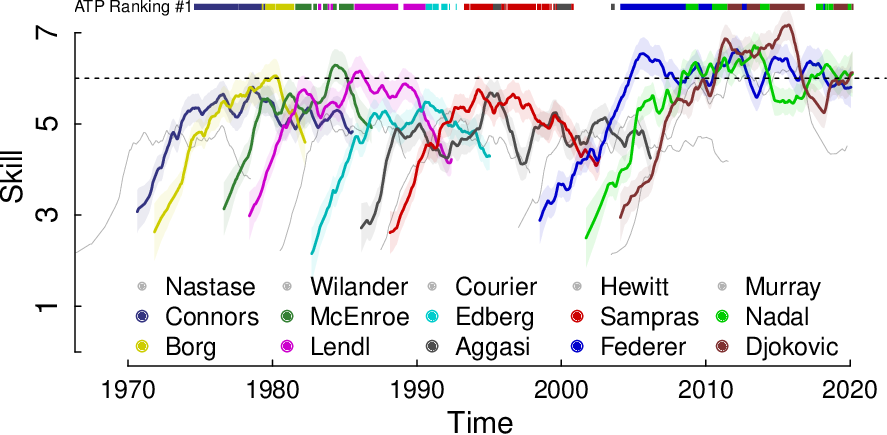
\includegraphics[width=.98\linewidth]{figures/atp}
    \caption{
    \en{Estimated learning curves for some famous male players. }%
    \es{Curvas de aprendizaje estimadas de algunos jugadores masculinos. }%
    }
    \label{fig:atp}
\end{subfigure}
\caption{
\en{\subref{tab:atp_weeks} Historical ranking according to the number of weeks that players reached the first position in the ATP's ranking until March 10, 2020. }%
\es{\subref{tab:atp_weeks} Ranking histórico de acuerdo a la cantidad de semanas que los jugadores alcanzaron la primera posición del ranking ATP hasta el 10 de marzo del 2020. }%
%
\en{\subref{fig:atp} Estimated skill of some of the historical ATP's leaders. }%
\es{\subref{fig:atp} Habilidad estimada de algunos de los líderes históricos de la ATP. }%
%
\en{The shaded area represents a standard deviation of uncertainty. }% 
\es{El área sombrada representa un desvío estandar de incertidumbre. }%
%
\en{The top bar indicates which player was at the top of the ATP's ranking. }%
\es{La barra superior indica cual jugador estaba en el primer puesto del ranking ATP. }%
%
\en{The dotted line, located at 6 skill points, is included to help compare the curves. }%
\es{La línea punteada, ubicada a los seis puntos de habilidad, se incluye para ayudar a comparar las curvas. }%
}
\end{figure}
%
\en{Table~\ref{tab:atp_weeks} shows the historical ranking of players in the top position of the ATP's ranking according to the number of weeks occupying the first position. The table is updated to the date of writing this manuscript and, as the ATP's tour was suspended due to the COVID-19, 22 weeks are excluded from consideration. }%
\es{La tabla~\ref{tab:atp_weeks} presenta el ranking histórico de acuerdo a la cantidad de semanas que los jugadores alcanzaron la primera posición del ranking ATP hasta el d\'ia de confecci\'on del presente documento. }%
%
\en{Figure~\ref{fig:atp} presents the estimated learning curves of some famous male players in ATP's history which we identified using different colors. }%
\es{En la figura~\ref{fig:atp} graficamos las curvas de aprendizaje de algunos jugadores famosos de la historia de la ATP, que identificamos usando diferentes colores. }%
%
\en{The top bar indicates which player was at the top of the ATP's ranking (the bar has no color when player number 1 is not included in our analysis). }%
\es{La barra superior indica cual jugador estaba en el primer puesto del ranking ATP (la barra no tiene color cuando el jugador numero 1 no está incluido en nuestro análisis). }%


% Parrafo
\en{ATP's ranking points are updated every Monday according to the prestige of the tournament and the stage reached. }%
\es{Los puntos de la clasificación de la ATP se actualizan semanalmente en función del prestigio del torneo y la fase alcanzada. }%
%
\en{Only during brief periods there is no coincidence between the estimated skill and the player who is at the top of the ATP's ranking, showing a good agreement between both methodologies. }%
\es{Sólo durante cortos períodos de tiempo no hay concordancia entre las estimaciones de habilidad y quién está en el primer puesto del ranking ATP, mostrando una buen acuerdo entre ambas metodologías. }%
%
\en{Notwithstanding, there are some notorious differences between estimated players' skills and the ATP's ranking, especially concerning the historical ranking shown in Table~\ref{tab:atp_weeks}. }%
\es{Sin embargo, hay algunas diferencias notables con respecto al ranking histórico que se muestra en la tabla~\ref{tab:atp_weeks}. }%
%
\en{On the one hand, Lleyton Hewitt's position in the historical ranking is the product of a window of opportunity opened around the year 2000, since his ability is relatively low in historical terms. }%
\es{La posición que obtiene Lleyton Hewitt en el ranking histórico de la ATP es producto de una ventana de oportunidad abierta cerca del año 2000, pues su habilidad es relativamente baja en términos históricos. }% 
%
\en{On the other hand, Andy Murray is the fourth most skilled player according to our estimations, but he only reaches 14th place in the historical ranking, just one place above Ilie N\u{a}stase. }%
\es{Por otro lado, Andy Murray, siendo el cuarto jugador más hábil, sólo ocupa el puesto 14 en la clasificación histórica de la ATP, sólo un lugar por encima de Ilie N\u{a}stase. }%

% Parrafo

\en{TrueSkill Through Time allows comparing the relative ability of players over time, unlike historical ATP's ranking and estimators based on the filtering approach (such as TrueSkill, Glicko, and IRT). }%
\es{TrueSkill Through Time permite comparar la habilidad relativa de los jugadores en el tiempo, a diferencia del ranking histórico de la ATP y de los estimadores basados en el enfoque de filtrado (como TrueSkill, Glicko e IRT). }%
%
\en{The learning curves share a similar pattern: they begin with rapid growth, reach an unstable plateau, and end with a slow decline (we hidden the last portion of the players who have long final stages for visualization purposes). }%
\es{Estas curvas de aprendizaje comparten un patrón similar: comienzan con un crecimiento rápido, alcanzan una meseta inestable, y terminan con una caída lenta (por razones de visualización hemos ocultado la última porción de los jugadores que tienen etapas finales largas). }%
%
\en{Individual learning curves enable recognizing special periods of crisis and prolonged stability of the professional players, and even the effects of emotional slumps such as those suffered by Aggasi and Djokovic. }%
\es{Las curvas de aprendizaje individuales permiten reconocer los períodos de crisis, estabilidad y éxito de los jugadores, e incluso los efectos de los bajones emocionales como los que sufrieron Aggasi y Djokovic. }%
%
% \en{Three major stages can be distinguished in Figure~\ref{fig:atp}: from the beginning until 1990, ii) between 1990 and 2003, iii) from 2003 onwards. }%
% \es{En la figura~\ref{fig:atp} se pueden observar tres grandes etapas: i) desde el comienzo hasta 1990, ii) entre 1990 y 2003, iii) desde 2003 en adelante. }%
% %
\en{It is worthwhile to note that the skill of tennis players did not increase abruptly over the years: contrary to what might have been expected, the players of the 1980s were more skilled than those of the 1990s, and reached a skill similar to what Federer, Nadal and Djokovic had in 2020, even though the latter reached higher values for a longer time.}%the players of the first zone are far more skilled than those of the 1990s (second zone), and those of the third zone noticeably surpassed all previous players in the history of ATP. }%
\es{Cabe destacar que la habilidad de los tenistas no aumentó bruscamente a lo largo de los años: en contra de lo que cabría esperar, los jugadores de la década de 1980 eran más hábiles que los de la década de 1990, y alcanzaron una habilidad similar a la que tenían Federer, Nadal y Djokovic en 2020, aunque estos últimos alcanzaron valores más altos durante más tiempo. }%
% \en{There is another difference in the third zone compared to the others regarding the duration of top players' careers: they can maintain their skill much longer than before. }%
% \es{COMPLETAR }%

% Parrafo

\en{In the previous example, we summarize the players' skills in a single dimension. }%
\es{En el ejemplo anterior resumimos la habilidad de los jugadores en una única dimensión. }% 
%
\en{TrueSkill Through Time allows estimating multi-dimensional skills. }%
\es{TrueSkill Through Time permite estimar habilidades multi-dimensionales. }%
%
\en{It is known that the ability of certain tennis players varies significantly depending on the surface. }%
\es{Sabemos que la habilidad de los jugadores de tenis puede variar significativamente según el tipo de suelo. }%
%
\en{To quantify this phenomenon, we propose modeling each player as a team composed of a generic player, who is included in all the games, and another player representing the ability of the player on a particular surface. } %
\es{Para cuantificar este fenómeno, proponemos modelar cada jugador como un equipo compuesto por un jugador genérico, que se incluye en todos los eventos, y otro jugador que representa la habilidad del jugador en una superficie particular. }% 
%
\en{For example, Nadal will be represented as a two-player team: \emph{Nadal\_generic} and \emph{Nadal\_clay} when playing on this kind of surface, and \emph{Nadal\_generic} and \emph{Nadal\_grass} when participating in the Wimbledon tournament. }%
\es{Por ejemplo, Nadal se representará como un equipo de dos jugadores: \emph{Nadal\_generic} y \emph{Nadal\_clay} cuando juegue en este tipo de superficie, y \emph{Nadal\_generic} y \emph{Nadal\_grass} cuando participe en el torneo de Wimbledon. }% 

\begin{lstlisting}[backgroundcolor=\color{julia!60},label=lst:atp_ground, caption={\en{Modeling multi-dimensional skills in ATP history}\es{Modelando habilidades multi-dimensionales en la historia de la ATP}}, belowskip=0.1cm, aboveskip=0.1cm]
players = Set(vcat((composition...)...))
priors = Dict([(p, Player(Gaussian(0., 1.6), 1.0, 0.036) ) for p in players])

composition_ground = [ r.double == "t" ? [[r.w1_id, r.w1_id*r.ground, r.w2_id, r.w2_id*r.ground],[r.l1_id, r.l1_id*r.ground, r.l2_id, r.l2_id*r.ground]] : [[r.w1_id, r.w1_id*r.ground],[r.l1_id, r.l1_id*r.ground]] for r in eachrow(data) ]   

h_ground = History(composition = composition_ground, times = dates, sigma = 1.0, gamma = 0.01, beta = 0.0, priors = priors)
convergence(h_ground, epsilon = 0.01, iterations=10)
\end{lstlisting}
%
\en{In this example, we keep the same prior as in code~\ref{lst:atp} for all the generic players, but in this code, we define them using the variable \texttt{priors}. }%
\es{En este ejemplo mantenemos el mismo prior para todos los jugadores genéricos, pero en esta ocasión los definidos usando la variable \texttt{priors}. }%
%
\en{We create the teams depending on whether the game is double or single similarly to code~\ref{lst:atp}, but now adding the specific surface skills of each player as their teammate (we use the operator \texttt{*} to concatenate strings). }%
\es{Al igual que en el código anterior (\ref{lst:atp}), creamos los equipos en función de si la partida es doble o simple, pero ahora añadiendo las habilidades específicas de cada jugador como su compañero de equipo (usamos el operador \texttt{*} para concatenar strings). }%
%
\en{As the specific surface skills are not defined in the variable \texttt{prior}, they are initialized using the default values defined in the class \texttt{History}. }%
\es{Como las habilidades específicas no están definidas en el diccionario \texttt{prior}, ellas van a ser inicializadas con los valores por defecto que le indicamos a la clase \texttt{History}. }%
%
\en{We also define \texttt{beta} as null for specific surface skills to avoid adding additional noise to the players' performance, keeping the scale of the estimates stable. }%
\es{Para ellos elegimos un \texttt{beta} nulo de modo tal de no agregar más ruido al rendimiento de los jugadores, manteniendo estable la escala de las estimaciones. }%
%
\en{We select a \texttt{sigma} that we consider sufficiently large and a dynamic factor \texttt{gamma} representing \SI{1}{\percent} of the prior uncertainty. }%
\es{Elegimos un \texttt{sigma} que consideramos suficientemente grande y una factor dinámico \texttt{gamma} que represente el 1\% de la incertidumbre a priori. }%
\begin{figure}[ht!]
    \centering
    \begin{subfigure}[t]{0.48\textwidth}
    \includegraphics[page={1},width=\linewidth]{figures/atp_ground}
    \caption{Nadal}
    \end{subfigure}
    \begin{subfigure}[t]{0.48\textwidth}
    \includegraphics[page={3},width=\linewidth]{figures/atp_ground}
    \caption{Djokovic}
    \end{subfigure}
    \caption{
    \en{Skill difference on the three main types of surface. }%
    \es{Diferencia de habilidad en los tres tipos de suelo principales. }%
    %
    \en{Each point on the $y$-axis represents a distance of one $\beta$, i.e. 76\% probability of winning. }%
    \es{Cada punto del eje $y$ representa una $\beta$ de distancia, es decir 76\% de probabilidad de ganar. }%
    }
    \label{fig:atp_ground}
\end{figure}

%
\en{In Figure~\ref{fig:atp_ground}, we show the skill difference that Nadal and Djokovic have in each of the three types of ground. }%
\es{En la figura~\ref{fig:atp_ground} mostramos la diferencia de habilidad que Nadal y Djokovic tiene entre los tres tipos de piso. }%
%
\en{Nadal has a notorious skill difference when playing on different surfaces. On the contrary, Djokovic has very similar skills in the three types. }%
\es{Podemos ver que Nadal tiene una diferencia de habilidad grande entre suelos, a diferencia de Djokovic que tiene habilidades muy similares en los tres tipos de suelo. }%
%
\en{The Nadal's skill difference between clay and grass grounds is greater than one $\beta$, which means at least 76\% difference in probability of winning compared to itself. }%
\es{La diferencia de habilidad de Nadal entre piso de polvo de ladrillo y pasto es mayor a un $\beta$, lo que significa una diferencia de al menos 76\% de probabilidad de ganar si lo comparamos consigo mismo. }%
%
\en{In the case of Nadal, it seems important to model the skill's multi-dimensionality, while in Djokovic's case it seems reasonable to summarize it in a single dimension. }%
\es{En el caso de Nadal parece importante modelar la multi-dimensionalidad de la habilidad, mientras que en el caso de Djokovic parece razonable resumir la habilidad en una única dimensión. }%
%
\en{To assess whether the complexity added by modeling multi-dimensionality is appropriate in general terms, we can compare the joint prior prediction of the models, calling the method \texttt{log\_evidence()} of the class \texttt{History}. }%
\es{Para evaluar si la complejidad que se agrega al modelar la multidimensional conviene en términos generales, podemos comparar la predicción a priori conjunta de los modelos, llamando al método \texttt{log\_evidence()} de la clase \texttt{History}. }%

%Parrafo

\en{In tennis, it is sufficient to summarize the skills in a single dimension since the prior prediction is maximized when the parameters of the surface's factors (i.e. $\sigma$ and $\gamma$) vanish. }%
\es{En tenis es suficiente resumir las habilidades en una única dimensión, dado que la predicción a priori se maximiza cuando los parámetros de los factores de piso, $\sigma$ y $\gamma$, se desvanecen. }%
%
\en{In other examples, where the multi-dimensionality of skills could be more relevant, it should be necessary to model the skills of all agents using different components. }%
\es{En otros ejemplos, donde la multidimensionalidad de las habilidades sea más relevante, convendrá separar la habildiad de todos los agente en diferentes componentes. }%
%
\en{If we consider only the games in which Nadal participates, optimality is achieved when the parameters take the values $\sigma=0.35$ and $\gamma=0$, meaning that it is necessary to model multidimensional skills ($\sigma>0$) but considering that their effect does not change over time ($\gamma = 0$). }%
\es{Si consideramos sólo las partidas en las que participa Nadal, la optimización se alcanza cuando los parámetros toman los valores $\sigma=0.35$ y $\gamma=0$, indicando que conivene modelar habilidades multidimensionales ($\sigma>0$) pero considerando que su efecto no cambia en el tiempo ($\gamma = 0$). }%
%
\en{In this scenario, Nadal's ability on Clay is $0.87\beta$ higher than on Hard and $1.05\beta$ higher than on Grass. }%
\es{En este escenario, la habilidad de Nadal en polvo de ladrillo es $0.87\beta$ mayor a la de cemento, y $1.05\beta$ mayor a la de pasto. }%
























































































%% -- Manuscript ---------------------------------------------------------------
%% - When describing longer chunks of code that are _not_ meant for execution
%%   (e.g., a function synopsis or list of arguments), the environment {Code}
%%   is recommended. Alternatively, a plain {verbatim} can also be used.
%%   (For executed code see the next section.)

\section{Models and software} 

\en{In this section, we provide the complete mathematical documentation of the TrueSkill Through Time model. }%
\es{En esta secci\'on ofrecemos la documentación matemática completa del modelo TrueSkill Through Time. }%
%
\en{The advantage of this model lies in the strict application of probability theory: all the assumptions are made explicit through a generative model, and the inference is solved only with the rules of probability, nothing more than the sum and the product rules. }%
\es{La ventaja de este modelo reside en la aplicación estricta de la teoría de la probabilidad: todos los supuestos se hacen expl\'icitos a trav\'es de un modelo generativo, y la inferencia se resuelve sólo con las regla de la probabilidad, nada más que las reglas de la suma y el producto. }%
%
\en{In section~\ref{sec:sumProductAlgorithm}, we introduce the \emph{sum-product algorithm}, which allows us to apply these rules to compute the marginal distributions, e.g. the posterior and the prior prediction. }%
\es{En la secci\'on~\ref{sec:sumProductAlgorithm} introducimos el \emph{sum-product algorithm}, que nos permite aplicar eficientemente estas reglas para computar las distribuciones marginales, e.g. el posterior y la predicción a priori. }%
%
\en{In section~\ref{sec:propiedades}, we list the properties that we will need to derive the marginal distributions of interest. }%
\es{En la secci\'on~\ref{sec:propiedades} enumeramos las propiedades que necesitaremos para derivar las distribuciones marginales de inter\'es. }%
%
\en{In section \ref{sec:Gaussian}, we introduce the operations of the class \texttt{Gaussian}, which does most of the computation. }%
\es{En las sección \ref{sec:Gaussian} introducimos las operaciones de la clases \texttt{Gaussian}, la que realiza la mayor parte del c\'omputo. }%
%
\en{In sections \ref{sec:2vs2}, \ref{sec:empate}, and \ref{sec:approximate_posterior}, we show how to solve the prior prediction and the exact posterior of an event, we introduce the model for a draw, and we explain how to approximate the exact posterior in events with two teams. }%
\es{En las secciones \ref{sec:2vs2}, \ref{sec:empate}, \ref{sec:approximate_posterior}, mostramos c\'omo resolver la predicci\'on a priori y el posterior exacto de un evento, incorporamos empate al modelo y explicamos c\'omo aproximar el posterior exacto en partidas con dos equipos. }%
%
\en{In section \ref{sec:iterative_posterior}, we explain the general multi-team solution which requires using an iterative algorithm. }%
\es{En la sección \ref{sec:iterative_posterior} explicamos la soluci\'on general multi-equipos, que requiere la aplicación de un algoritmo iterativo. }%
%
\en{In section~\ref{sec:throughTime}, we justify the mathematical steps required to solve the full TrueSkill Through Time model. }%
\es{En la secci\'on~\ref{sec:throughTime} justificamos los pasos matemáticos requeridos para resolver el modelo TrueSkill Through Time completo. }%

\subsection{Sum-product Algorithm} \label{sec:sumProductAlgorithm}

\en{The \emph{sum-product algorithm}~\citep{Kschischang2001} takes advantage of the structure of the joint probability distribution, imposed by the causal model, to efficiently apply the rules of probability. }%
\es{El \emph{sum-product algorithm}~\citep{Kschischang2001} aprovecha la estructura de la distribuci\'on de probabilidad conjunta, impuesta por el modelo causal, para aplicar eficientemente las reglas de la probabilidad. }%
%
\en{Any model can be factorized into the product of conditional probabilities. }%
\es{Cualquier modelo puede factorizarse en el producto de probabilidades condicionales. }%
%
\en{As the variables are independent, our model (figure~\ref{fig:generative_model}) can be factorized as,}
\es{Haciendo uso de las independencias entre las variables, nuestro modelo (figura~\ref{fig:generative_model}) puede factorizarse como,}
%
\begin{equation} \label{eq:factorization}
 p(\bm{s},\bm{p},d,r) = p(s_1)p(s_2)p(p_1|s_1)p(p_2|s_2)p(d|\bm{p})P(r|d)
\end{equation}
%
\en{In Fig.~\ref{fig:factor_graph}, we show this factorization graphically. }%
\es{En la figura~\ref{fig:factor_graph} mostramos esta factorizaci\'on graficamente. }%
%
\en{These representations, known as \emph{factor graphs}, have two kinds of nodes: variable-type nodes (white circles) and function-type nodes (black squares). }%
\es{Este tipo de representaciones, conocidas como \emph{factor graph}, son gr\'afos con dos tipos de nodos: nodos variables (círculos blancos), y nodos funciones (cuadrados negros). }%
%
\en{The edge between node variables and node functions represents the mathematical relationship ``the variable $v$ is an argument of the function $f$''. }%
\es{Los ejes entre nodos variables y nodos funciones representan la relaci\'on matem\'atica ``la variable $v$ es argumento de la funci\'on $f$''. }%
%
\begin{figure}[ht!]
\centering \small
    \tikz{         
%         \node[const, above=of fr] (nfr) {$f_r$}; %
% 	\node[const, above=of nfr] (dfr) {\large $\mathbb{I}(d >0)$}; %
        
    \node[factor] (fr) {} ; 
    \node[const, left=of fr] (nfr) {\normalsize $P(r|d)$}; 
    \node[const, right=of fr] (dfr) {\normalsize \hspace{2.4cm} $P(r|d)=\mathbb{I}(d>0)$}; 

    \node[latent, above=of fr, yshift=-0.6cm] (d) {$d$} ; %
    \node[const, left=of d, xshift=-1.35cm] (d_name) {\small \en{Difference}\es{Diferencia}:};
    
    
    \node[factor, above=of d,yshift=-0.6cm] (fd) {} ; 
    \node[const, left=of fd] (nfd) {\normalsize $p(d|\bm{p})$}; 
    \node[const, right=of fd] (dfd) {\normalsize \hspace{2.4cm} $p(d|\bm{p}) =\delta(d=p_1-p_2) $}; 
    
    
    \node[latent, above=of fd, xshift=-0.8cm, yshift=-0.6cm] (p1) {$p_1$} ; %
    \node[latent, above=of fd, xshift=0.8cm, yshift=-0.6cm] (p2) {$p_2$} ; %
    \node[const, left=of p1, xshift=-0.55cm] (p_name) {\small \en{Performance}\es{Rendimiento}:}; 

    \node[factor, above=of p1 ,yshift=-0.6cm] (fp1) {} ; 
    \node[factor, above=of p2 ,yshift=-0.6cm] (fp2) {} ; 
    
    \node[latent, above=of fp1,yshift=-0.6cm] (s1) {$s_1$} ; %
    \node[latent, above=of fp2,yshift=-0.6cm] (s2) {$s_2$} ; %
    
    \node[factor, above=of s1 ,yshift=-0.6cm] (fs1) {} ; 
    \node[factor, above=of s2 ,yshift=-0.6cm] (fs2) {} ; 
    
    
    \node[const, left=of fp1] (nfp1) {\normalsize $p(p_1|s_1)$};
    \node[const, right=of fp2] (nfp2) {\normalsize $p(p_2|s_2)$};
    \node[const, right=of fp2] (dfp2) {\normalsize \hspace{1.6cm} $p(p_i|s_i)=\N(p_i|s_i,\beta^2)$};

    \node[const, left=of s1, xshift=-.85cm] (s_name) {\small \en{Skill}\es{Habilidad}:}; 
    
    \node[const, left=of fs1] (nfs1) {\normalsize $p(s_1)$};
    \node[const, right=of fs2] (nfs2) {\normalsize $p(s_2)$};
    \node[const, right=of fs2] (dfs) {\normalsize \hspace{1.6cm} $p(s_i) = \N(s_i|\mu_i,\sigma_i^2)$};

    
    \edge[-] {d} {fr};
    \edge[-] {p1,p2,d} {fd};
    \edge[-] {fp1} {p1,s1};
    \edge[-] {fp2} {p2,s2};
    \edge[-] {fs1} {s1};
    \edge[-] {fs2} {s2};
}
     \caption{%
     \en{Graphical way of representing the factorization of joint distribution induced by the basic causal model, represented by Eq.~\eqref{eq:factorization}. }%
     \es{Forma gráfica de representar la factorizaci\'on de la distribución conjunta inducida por el modelo causal básico (ecuación~\eqref{eq:factorization}). }%
     %
     \en{Black squares represent the functions, white circles represent the variables, and the edges between them represent the mathematical relationship ``the variable is the argument of the function''. }%
     \es{Los cuadrados negros representan las funciones, los c\'irculos blancos representan las variable, y los ejes entre ellos representan la relaci\'on matem\'atica ``la variable es argumento de la funci\'on''. }%
     %
     }
    \label{fig:factor_graph}
\label{modelo}
\end{figure} 
%
\en{In our case, we want to compute two marginals, the proportional posterior of the skills $p(s_i, r)$ and the prior probability of the result $p(r)$. }%
\es{En nuestro caso querermos computar dos marginales, el posterior proprocional de las habilidades $p(s_i, r)$ y la probabilidad a priori del resultado $p(r)$. }%
%
\en{The \emph{sum-product algorithm} is a general way of breaking down the rules of probability as messages locally sent between the nodes of the \emph{factor graph}. }%
\es{El \emph{sum-product algorithm} es una forma general de descomponer las reglas de la probabilidad como mensajes que se env\'ian los nodos del \emph{factor graph}. }%
%
\en{There are two types of messages: those sent by variable-type nodes to their function-type neighbors ($m_{v \rightarrow f}(v)$) and the ones that function-type nodes send to their variable-type neighbors ($m_{f \rightarrow v}(v)$). }%
\es{Hay dos tipos de mensajes: los mensajes que envian los nodos variables a sus funciones vecinas ($m_{v \rightarrow f}(v)$); y los mensajes que env\'ian los nodos funciones a sus variables vecinas ($m_{f \rightarrow v}(v)$). }%
%
\en{The former partially performs the product rule. }%
\es{El primero codifica una porci\'on de la regla del producto. }%
%
\begin{equation*}\label{eq:m_v_f} \tag{\text{\en{product step}\es{paso del producto}}}
m_{v \rightarrow f}(v) = \prod_{h \in n(v) \setminus \{f\} } m_{h \rightarrow v}(v)
\end{equation*}
%
\en{where $n(v)$ represents the set of neighbor nodes to $v$. }%
\es{donde $n(v)$ representa el conjunto de vecinos del nodo $v$. }%
%
\en{In a brief, the messages sent by the variable-type node $v$ are simply the product of the messages that $v$ receives from the rest of their neighbors $h \in n(v)$ except $f$. }%
\es{En pocas palabras, los mensajes que env\'ia una variables $v$ es simplemente la multiplicaci\'on de los mensajes que recibi\'o del resto de sus vecinos $h \in n(v)$ salvo $f$. }%
%
\en{The messages sent by the function-type nodes encode a portion of the sum rule. }%
\es{Los mensajes que env\'ian los nodos funciones codifican una parte de la regla de la suma. }%
%
\begin{equation*}\label{eq:m_f_v}  \tag{\text{\en{sum step}\es{paso de la suma}}}
m_{f \rightarrow v}(v) = \int \cdots \int \Big( f(\bm{h},v) \prod_{h \in n(f) \setminus \{v\} } m_{h \rightarrow f}(h) \Big) \,  d\bm{h}
\end{equation*}
%
\en{where $\bm{h} = n(f)\setminus \{v\}$ is the set of all neighbors to $f$ except $v$, and $f(\bm{h},v)$ represents the function $f$, evaluated in all its arguments. }%
\es{donde $\bm{h} = n(f)\setminus \{v\}$ es el conjunto de todos los vecinos de $f$ salvo $v$, y $f(\bm{h},v)$ representa la funci\'on $f$, evaluada en todos sus argumentos. }%
%
\en{The messages sent by the function-type node $f$ to a neighboring variable-type node $v$ is simply the integration (or sum) over $\bm{h}$ of the product of itself and all the messages that $f$ receives from the rest of its neighbors $\bm{h}$ except $v$. }%
\es{En pocas palabras, los mensajes que envía una funci\'on $f$ a una variable vecina $v$ es simplemente la integraci\'on (o suma) sobre $\bm{h}$ del producto de sí mismo con todos los mensajes que $f$ recibe del resto de sus vecinos $\bm{h}$ salvo $v$. }%
%
\en{Finally, the marginal probability distribution of a variable $v$ is simply the product of the messages that $v$ receives from all its neighbors. }%
\es{Finalmente, la distribuci\'on de probabilidad marginal de una variable $v$ es simplemente la multiplicaci\'on de los mensajes que $v$ recibe de todos sus vecinos. }%
%
\begin{equation*}\label{eq:marginal}  \tag{\text{\en{marginal probability}\es{probabilidad marginal}}}
p(v) = \prod_{h \in n(v)} m_{h \rightarrow v}
\end{equation*}
%
\en{This algorithm encodes the minimum number of steps required to calculate any marginal probability distribution. }%
\es{Este algoritmo codifica la m\'inima cantidad de pasos que se requieren para calcular cualquier distribuci\'on de probabilidad marginal. }%


\subsection{\en{Mathematical Properties and Notation}\es{Propiedades matem\'aticas y notaci\'on}}\label{sec:propiedades}

\en{The efficiency of TrueSkill Through Time is based on the analytical computation of marginal probabilities. }%
\es{La eficiencia de TrueSkill Through Time se obtiene gracias que las marginales se pueden computar de forma analítica. }%
%
\en{In this section, we list the properties that we need to derive the exact and the approximate messages that arise from the sum-product algorithm. }%
\es{En esta secci\'on enumeramos las propiedades que necesitamos para derivar los mensajes exactos y aproximados que surgen del \emph{sum-product algorithm}. }%
%
\en{The first property states that the product of two Gaussian distributions, both evaluated at the same point $x$, can be expressed as the product of two other Gaussian distributions with only one of them evaluated at $x$. }%
\es{La primera propiedad establece que el producto de dos distribuciones gaussianas, ambas evaluadas en el mismo punto $x$, pueden expresarse como la producto de otras dos distribuciones gaussianas con sólo una de ellas evaluada en $x$. }%
%
\begin{equation*}\label{eq:gaussian_product} \tag{\text{\en{Gaussian product}\es{Producto de gaussianas}}}
\N(x|\mu_1,\sigma_1^2)\N(x|\mu_2,\sigma_2^2) \overset{\ref{multiplicacion_normales}}{=} \N(\mu_1|\mu_2,\sigma_1^2+\sigma_2^2) \N(x|\mu_{*},\sigma_{*}^2)
\end{equation*}
%
\en{where}\es{con} $\mu_{*} = \frac{\mu_1}{\sigma_1^2} + \frac{\mu_2}{\sigma_2^2}$ y $\sigma_{*}^2 = \left(\frac{1}{\sigma_1^2} + \frac{1}{\sigma_2^2} \right)^{-1}$.
%
\en{Something similar occurs with the division of two Gaussian distributions, both evaluated at the same point $x$. }%
\es{Algo similar ocurre con la división de dos distribuciones gaussianas, ambas evaluadas en el mismo punto $x$. }%
\begin{equation*}\label{eq:gaussian_division} \tag{\text{\en{Gaussian division}\es{División de gaussianas}}}
\N(x|\mu_1,\sigma_1^2)/\N(x|\mu_2,\sigma_2^2) \overset{\ref{sec:division_normales}}{\propto} \N(x|\mu_{\div},\sigma_{\div}^2)/\N(\mu_1|\mu_2,\sigma_1^2+\sigma_2^2) 
\end{equation*}
%
\en{where}\es{con} $\mu_{\div} = \frac{\mu_1}{\sigma_1^2} - \frac{\mu_2}{\sigma_2^2}$ y $\sigma_{\div}^2 = \left(\frac{1}{\sigma_1^2} - \frac{1}{\sigma_2^2} \right)^{-1}$.

\en{The indicator function $\mathbb{I}(\cdot=\cdot)$ is $1$ when equality is true and $0$ otherwise. }%
\es{La funci\'on indicadora $\mathbb{I}(\cdot=\cdot)$ vale $1$ cuando la igualdad es verdadera y $0$ en caso contrario. }%
%
% \en{When we can use it to replace variable within an integral,}
% \es{Cuando podemos usarla para remplazar variable dentro de una integral,}
% %
% \begin{equation}\label{eq:integral_con_indicadora} \tag{\text{\en{Indicator function}\es{Función indicadora}}}
% \begin{split}
%  \iint  \mathbb{I}(x=h(y,z)) f(x) g(y)\, dx\, dy = \int f(h(y,z)) g(y) dy
%  \end{split}
% \end{equation}
% %
% \en{the dimensionality of the problem is reduced. }%
% \es{la dimensionalidad del problema se reduce. }%
% %
\en{It represents probabilities distributions of non-random discrete variables, such as the result of the games given the difference of performances $p(r|d)$. }%
\es{Se usa para representar distribuciones de probabilidad de variables discretas no aleatorias, como el resultado de las partidas dada la diferencia de desempeños $p(r|d)$. }%
%
\en{Similarly, the Dirac delta function $\delta(\cdot=\cdot)$ represents probabilities distributions of non-random continuous variables, such as the difference of performances given the agents' performances $p(d|\bm{p})$. }%
\es{De la misma forma, la función delta de Dirac $\delta(\cdot=\cdot)$ se usa para representar distribuciones de probabilidad de variables continuas no aleatoria, es la diferencia de desempeños dados los rendimientos de los agentes $p(d|\bm{p})$. }%
%
\en{If we can use it to replace variable within an integral,}
\es{Cuando permite remplazar variable dentro de una integral,}
%
\begin{equation*}\label{eq:integral_con_dirac} \tag{\text{\en{Dirac delta function}\es{Función delta de dirac}}}
\begin{split}
 \iint  \delta(x=h(y,z)) f(x) g(y)\, dx\, dy = \int f(h(y,z)) g(y) dy
 \end{split}
\end{equation*}
%
\en{the dimensionality of the problem is reduced. }%
\es{la dimensionalidad del problema se reduce. }%
%
\en{We will also use the properties derived from the symmetry of Gaussians. }%
\es{Usaremos además las propiedades que se derivan de la simetría de gaussianas. }%
%
\begin{equation*}\label{eq:simetria} \tag{\text{\en{Gaussian symmentry}\es{Simetría de gaussianas}}}
 \N(x|\mu,\sigma^2) = \N(\mu|x,\sigma^2) = \N(-\mu|-x,\sigma^2) = \N(-x|-\mu,\sigma^2) 
\end{equation*}
%
\en{The Gaussian standardization,}
\es{La estandizarización de la gaussiana,}
\begin{equation*}\label{eq:estandarizar} \tag{\text{\en{Gaussian standarization}\es{Estandarización de gaussianas}}}
  \N(x|\mu,\sigma^2) = \N((x-\mu)/\sigma | 0, 1)
\end{equation*}
%
\en{Equality between the Gaussian distribution and the derivative of their cumulative distribution,}
\es{La igualdad entre la distribución gaussiana y la derivada de la su acumulada,}
\begin{equation*}\label{eq:phi_norm} \tag{\text{\en{Derivative of the cumulative Gaussian}\es{Derivada de la gaussiana acumulada}}}
 \frac{\partial}{\partial x} \Phi(x|\mu,\sigma^2) = \N(x|\mu,\sigma^2)
\end{equation*}
%
\en{which is valid by definition. }%
\es{que vale por definición. }%
%
\en{The symmetry of the cumulative Gaussian distribution. }%
\es{La simetría de la distribución gaussiana acumulada. }%
\begin{equation*}\label{eq:phi_simetria} \tag{\text{\en{Symmetry of the cumulative Gaussian}\es{Simetría de la gaussiana acumulada}}}
\Phi(0|\mu,\sigma^2) = 1-\Phi(0|-\mu,\sigma^2)
\end{equation*}

\subsection{\en{The Gaussian Class}\es{La clase gaussiana}}\label{sec:Gaussian}

\en{The \texttt{Gaussian} class does most of the computation of the packages. }%
\es{La clase \texttt{Gaussian} realiza la mayor parte del c\'omputo en todos los paquetes. }%
%
\en{It is characterized by the mean (\texttt{mu}) and the standard deviation (\texttt{sigma}). }%
\es{Se representa mediante dos par\'ametros, la media y el desv\'io estandar. }%
% %
\begin{lstlisting}[backgroundcolor=\color{all},label=lst:N1_N2, caption={\en{Initialization of Gaussians distributions}\es{Inicialización de distirbuciones gaussianas}}, belowskip=-1.0 \baselineskip, aboveskip=-0 \baselineskip]
\end{lstlisting}
\begin{lstlisting}[backgroundcolor=\color{all}, belowskip=0.0 \baselineskip]
N1 = Gaussian(mu = 1.0, sigma = 1.0); N2 = Gaussian(1.0, 2.0)  
\end{lstlisting}
%
\en{The class overwrites the addition (\texttt{+}), subtraction (\texttt{-}), product (\texttt{*}), and division (\texttt{/}) to compute the marginal distributions used in the TrueSkill Through Time model. }%
\es{La clase sobreescribe los operadores suma (\texttt{+}), resta (\texttt{-}), producto (\texttt{*}) y divisi\'on (\texttt{/}) con las principales propiedades requeridas para computar las distribuciones marginales en el modelo TrueSkill Through Time. }%
%
\begin{equation*} \tag{\texttt{N1 * N2}}
 \N(x|\mu_1,\sigma_1^2)\N(x|\mu_2,\sigma_2^2) \overset{\ref{multiplicacion_normales}}{\propto} \N(x|\mu_{*},\sigma_{*}^2)
\end{equation*}
%
\begin{equation*} \tag{\texttt{N1 / N2}}
 \N(x|\mu_1,\sigma_1^2)/\N(x|\mu_2,\sigma_2^2)  \overset{\ref{sec:division_normales}}{\propto} \N(x|\mu_{\div},\sigma_{\div}^2)
\end{equation*} 
%
\vspace{-0.3cm}
%
\begin{equation*} \tag{\texttt{N1 + N2}} \label{eq:suma_normales}
\begin{split}
\iint \delta(t=x + y) \N(x|\mu_1, \sigma_1^2)\N(y|\mu_2, \sigma_2^2) dxdy \overset{\text{\ref{suma_normales_induccion}}}{=} \N(t|\mu_1+\mu_2,\sigma_1^2 + \sigma_2^2)
\end{split}
\end{equation*}
%
\vspace{-0.5cm}
%
\begin{equation*} \tag{\texttt{N1 - N2}} \label{eq:resta_normales}
\begin{split}
\iint \delta(t = x - y) \N(x|\mu_1, \sigma_1^2)\N(y|\mu_2, \sigma_2^2) dxdy \overset{\text{\ref{suma_normales_induccion}}}{=} \N(t|\mu_1 - \mu_2,\sigma_1^2 + \sigma_2^2)
\end{split}
\end{equation*}
%
\en{Although these properties are widely known, we attach their complete demonstrations in the supplemental material. }%
\es{Aunque estas propiedades son ampliamente conocidas, adjuntamos sus demostraciones completas en el material suplementario. }%

\subsection{\en{The Exact Solution for Events with Two Teams}\es{La solución exacta para eventos con dos equipos}}\label{sec:2vs2}

% \en{TrueSkill allows to estimate the skill of individuals even when they play in teams. }%
% \es{TrueSkill permite estimar la habilidad de los individuos incluso cuando estos juegan en equipo. }%
%
\en{In the presence of teams, the Elo model assumes that a team's performance is the sum of the performance of its members. The team with the highest performance wins, $r = (t_i> t_j)$. }%
\es{En presencia de equipos, el modelo Elo supone que el desempeño de los equipos $t$ es la suma de los desempeños de sus integrantes, y que el equipo con mayor desempeño gana, $r = (t_i > t_j)$. }%
%
\en{In Fig.~\ref{fig:modelo_trueskill_2vs2}, we show the graphical factorization of the Elo team model. }%
\es{En la figura~\ref{fig:modelo_trueskill_2vs2} mostramos la factorizaci\'on gr\'afica del modelo Elo que incorpora equipos. }% 
%
\begin{figure}[ht!]
  \centering
  \scalebox{.9}{
  \tikz{
      
        \node[factor] (fr) {} ;
        \node[const, right=of fr] (nfr) {$f_{r}$}; %
	
	\node[latent, above=of fr, yshift=-0.4cm] (d) {$d$} ; %
        \node[factor, above=of d, yshift=-0.4cm] (fd) {} ;
        \node[const, above=of fd] (nfd) {$f_{d}$}; %
	
        
        \node[latent, left=of fd,xshift=0.4cm] (ta) {$t_a$} ; %
        \node[factor, left=of ta,xshift=0.4cm] (fta) {} ;
        \node[const, above=of fta] (nfta) {$f_{t_a}$}; %
        
        \node[latent, left=of fta,yshift=1cm,xshift=0.4cm] (p1) {$p_1$} ; %
        \node[factor, left=of p1,xshift=0.4cm] (fp1) {} ;
        \node[const, above=of fp1] (nfp1) {$f_{p_1}$}; %
        
        \node[latent, left=of fp1,xshift=0.4cm] (s1) {$s_1$} ; %
        \node[factor, left=of s1,xshift=0.4cm] (fs1) {} ;
	\node[const, above=of fs1] (nfs1) {$f_{s_1}$}; %
     
        \node[latent, left=of fta,yshift=-1cm,xshift=0.4cm] (p2) {$p_2$} ; %
        \node[factor, left=of p2,xshift=0.4cm] (fp2) {} ;
        \node[const, above=of fp2] (nfp2) {$f_{p_2}$}; %
        
        \node[latent, left=of fp2,xshift=0.4cm] (s2) {$s_2$} ; %
        \node[factor, left=of s2,xshift=0.4cm] (fs2) {} ;
	\node[const, above=of fs2] (nfs2) {$f_{s_2}$}; %
        
            
        \node[latent, right=of fd,xshift=-0.4cm] (tb) {$t_b$} ; %
        \node[factor, right=of tb,xshift=-0.4cm] (ftb) {} ;
        \node[const, above=of ftb] (nftb) {$f_{t_b}$}; %
        
        \node[latent, right=of ftb,yshift=1cm,xshift=-0.4cm] (p3) {$p_3$} ; %
        \node[factor, right=of p3,xshift=-0.4cm] (fp3) {} ;
        \node[const, above=of fp3] (nfp3) {$f_{p_3}$}; %
        
        \node[latent, right=of fp3,xshift=-0.4cm] (s3) {$s_3$} ; %
        \node[factor, right=of s3,xshift=-0.4cm] (fs3) {} ;
	\node[const, above=of fs3] (nfs3) {$f_{s_3}$}; %
     
        \node[latent, right=of ftb,yshift=-1cm,xshift=-0.5cm] (p4) {$p_4$} ; %
        \node[factor, right=of p4,xshift=-0.4cm] (fp4) {} ;
        \node[const, above=of fp4] (nfp4) {$f_{p_4}$}; %
        
        \node[latent, right=of fp4,xshift=-0.4cm] (s4) {$s_4$} ; %
        \node[factor, right=of s4,xshift=-0.4cm] (fs4) {} ;
	\node[const, above=of fs4] (nfs4) {$f_{s_4}$}; %
     
        \edge[-] {fr} {d};
	\edge[-] {d} {fd};
	
        \edge[-] {fd} {ta};
        \edge[-] {ta} {fta};
        \edge[-] {fta} {p1};
        \edge[-] {p1} {fp1};
        \edge[-] {fp1} {s1};
        \edge[-] {s1} {fs1};
        \edge[-] {fta} {p2};
        \edge[-] {p2} {fp2};
        \edge[-] {fp2} {s2};
        \edge[-] {s2} {fs2};
        	
	\edge[-] {fd} {tb};
        \edge[-] {tb} {ftb};
        \edge[-] {ftb} {p3};
        \edge[-] {p3} {fp3};
        \edge[-] {fp3} {s3};
        \edge[-] {s3} {fs3};
        \edge[-] {ftb} {p4};
        \edge[-] {p4} {fp4};
        \edge[-] {fp4} {s4};
        \edge[-] {s4} {fs4};
        
	
	\node[const, below=of fr,xshift=7cm,yshift=-0.3cm] (dfr) { $f_r = \mathbb{I}(d>0)$}; %
	\node[const, left=of dfr,xshift=-0.5cm] (dfd) {$f_d = \delta(d=t_a - t_b)$}; %
	\node[const, left=of dfd,xshift=-0.5cm] (dft) {$f_{t_e} = \delta(t_e = \sum_{i \in A_e} p_i)$}; %
        \node[const, left=of dft,xshift=-0.5cm] (dfp) {$f_{p_i} = \N(p_i|s_i,\beta^2)$}; %
        \node[const, left=of dfp,xshift=-0.5cm] (dfs) {$f_{s_i} = \N(s_i|\mu_i,\sigma^2)$}; %
   }
   }
  \caption{
  \en{Factor graph of a game with two teams with two players each. }%
  \es{Factorizaci\'on gr\'afica de una partida con dos equipos de dos jugadores. }%
  %
  \en{The Elo's team model incorporate a new variable, $t$, that models the team performance. }%
  \es{El modelo Elo incorpora una variable nueva, $t$, que modela el desempeño de los equipos. }%
  }
  \label{fig:modelo_trueskill_2vs2}
\end{figure}
%
\en{In this example, we have two teams with two players each. }%
\es{En este ejemplo, tenemos dos equipos con dos jugadores cada uno. }%
%
\en{Every game with two teams has an analytical solution. }%
\es{Toda partida con dos equipos tiene soluci\'on analítica exacta. }%


% Parrafo

%
\en{In this section, we show the steps to compute the exact evidence and likelihoods for a game with two teams. }%
\es{En esta secci\'on mostramos los pasos para calcular la evidencia exacta y los likelihoods exactos de una partida con dos equipos. }%
%
\en{We only need the \emph{sum-product algorithm} and the properties mentioned above. }%
\es{Sólo necesitamos el \emph{sum-product algorithm} y las propiedades arriba mencionadas. }%
%
\en{We will start first with the ``descending'' messages, from the priors to the result until computing the evidence. Then, we continue with the ``ascending'' messages, from the observed result and to the priors until compute the posterior of each agent. }%
\es{Empezaremos primero con los mensajes ``descendentes'', desde los priors al resultado, hasta calcular la evidencia, y seguiremos con los mensajes ``ascendentes'', desde el resultado observado a los priors, hasta calcular el posterior de cada agente. }%

\paragraph{\en{Descending messages}\es{Mensajes descendentes}. }%

\en{Following the \ref{eq:m_f_v} of the sum-product algorithm and the factorization of the model displayed in Fig.~\ref{fig:modelo_trueskill_2vs2}, we can see that the messages sent by the skill factors $f_{s_i}$ to the variable $s_i$ are just the priors. }%
\es{Siguiendo el~\ref{eq:m_f_v} del \emph{sum-product algorithm} y la factorizaci\'on del modelo presentado en la figura~\ref{fig:modelo_trueskill_2vs2}, podemos ver que los mensajes que envían los factores de habilidad $f_{s_i}$ a la variable $s_i$ no son otra cosa m\'as que el prior. }%
%
\begin{equation*}\label{eq:m_fs_s} \tag{\texttt{prior}}
 m_{f_{s_i} \rightarrow s_i}(s_i) = \N(s_i| \mu_i, \sigma_i^2)
\end{equation*}
%
\en{We have access to this message by calling the \texttt{prior} attribute of the \texttt{Player} class. }%
\es{Tenemos acceso a este mensaje llamando al atributo \texttt{prior} de la clase \texttt{Player}. }%
%
\en{Following the~\ref{eq:m_v_f} of the sum-product algorithm and the factorization of the model, the message sent by the variable $s_i$ to the performance factor $f_{p_i}$ is the prior. }%
\es{Podemos ver también, siguiendo el~\ref{eq:m_v_f} del \emph{sum-product algorithm} y la factorizacion del modelo, que el mensaje que envía la variable $s_i$ al factor rendimiento $f_{p_i}$ es nuevamente el prior. }%
%
\en{Since it is trivial to calculate the messages sent by the variables (they are the product of the messages received from behind), we do not include them. }%
\es{Debido a que es trivial calcular los mensajes que envían las variables (siempre es el producto de los mensajes que reciben de atrás), vamos a evitar escribirlos. }%
%
\en{Then, the message sent by the performance factors $f_{p_i}$ to the variable $p_i$ is: }%
\es{Veamos entonces el mensaje que env\'ian los factores rendimiento $f_{p_i}$ a su variable $p_i$. }%
%
\begin{equation*}\label{eq:m_fp_p} \tag{\texttt{performance()}}
m_{f_{p_i} \rightarrow p_i}(p_i) = \int \N(p_i| s_i, \beta^2) \N(s_i| \mu_i, \sigma_i^2) ds_i = \N(p_i|\mu_i,\beta^2 + \sigma_i^2)
\end{equation*}
%
\en{We have access to these messages through the \texttt{performance()} method of the \texttt{Player} class. }%
\es{Tenemos acceso a estos mensajes mediante el método \texttt{performance()} de la clase \texttt{Player}. }%
%
\begin{lstlisting}[backgroundcolor=\color{white},label=lst:performance, caption={\en{Computing the individual prior performance}\es{Computando el desempeño individual a priori}}, belowskip=-1.0 \baselineskip, aboveskip=0.0 \baselineskip]
\end{lstlisting}
\begin{paracol}{3}
\begin{lstlisting}[backgroundcolor=\color{julia!60}]
p1 = performance(a1)
p2 = performance(a2)
p3 = performance(a3)
p4 = performance(a4)
\end{lstlisting}
  \switchcolumn
\begin{lstlisting}[backgroundcolor=\color{python!60}]
p1 = a1.performance()
p2 = a2.performance()
p3 = a3.performance()
p4 = a4.performance()
\end{lstlisting}
   \switchcolumn
\begin{lstlisting}[backgroundcolor=\color{r!50}]
p1 = performance(a1)
p2 = performance(a2)
p3 = performance(a3)
p4 = performance(a4)
\end{lstlisting}  
\end{paracol}
%
\en{where the agents \texttt{a1}, \texttt{a2}, \texttt{a3}, and \texttt{a4} were initialized in code~\ref{lst:player}. }%
\es{donde los agentes \texttt{a1}, \texttt{a2}, \texttt{a3} y \texttt{a4}, fueron inicializados en el código~\ref{lst:player}. }%
%
\en{The message sent by the team factors $f_{t_e}$ to the team variable $t_e$ is an integral over all the individual performance variables,}
\es{El mensaje que envían los factores equipos $f_{t_e}$ a la variable equipo $t_e$ es una integral sobre todas las variables de desempeño individual,}
%
\begin{equation*} \label{eq:m_ft_t} \tag{\texttt{ta = p1 + p2}}
\begin{split}
 m_{f_{t_e} \rightarrow t_e}(t_e) &= \iint \delta(t_e = p_i + p_j) \N(p_i|\mu_i,\beta^2 + \sigma_i^2)\N(p_j|\mu_j,\beta^2 + \sigma_j^2) dp_idp_j  \\ &=  \N(t_e|\underbrace{\mu_i+\mu_j}_{\text{\normalsize $\mu_e\phantom{^2}$}}, \underbrace{2\beta^2 + \sigma_i^2 + \sigma_j^2}_{\text{\normalsize $\sigma_e^2$}})
\end{split}
\end{equation*}
%
\en{where the Dirac delta function imposes the constraint that the sum of the individual performances equals a constant team performance value $t_e$. }%
\es{donde la función delta de Dirac impone la restricción de que la suma de los desempeños individuales sea igual a un valor de rendimiento del equipo $t_e$ constante. }%
%
\en{Applying the already presented properties, we can solve this integral analytically, obtaining the prior performance of the teams, which is a Gaussian distribution centered on the sum of the mean estimates $\mu_e = \mu_i + \mu_j$ with a variance $\sigma_e^2$ including both the uncertainties of the estimates (i.e. $\sigma_i^2 + \sigma_j^2$) and the variance of the individual performances (i.e. 2$\beta^2$). }%
\es{Haciendo uso de las propiedades podemos resolver esta integral de forma analítica, obteniendo como resultado que el desempeño a priori de los equipos es una distribución gaussiana centrada en la suma de las estimaciones medias $\mu_e = \mu_i + \mu_j$ con una varianza que incluye tanto las incertidumbres de las estimaciones, $\sigma_i^2 + \sigma_j^2$, como la varianza de los rendimientos individuales, $\beta^2 + \beta^2$. }%
%
\en{We have access to this message using the operator \texttt{+} of the class \texttt{Gaussian} to sum the agents' performances,}
\es{Tenemos acceso a este mensaje cuando usamos el operador \texttt{+} de la clase \texttt{Gaussian} para sumar los desempeños de los agentes,}
%
\begin{lstlisting}[backgroundcolor=\color{white},label=lst:team_performance, caption={\en{Computing the team prior performance}\es{Computando el desempeño a priori de los equipos}}, belowskip=-1.0 \baselineskip, aboveskip=0.0 \baselineskip]
\end{lstlisting}
\begin{lstlisting}[backgroundcolor=\color{all}]
ta = p1 + p2; tb = p3 + p4
\end{lstlisting}
%
\en{The next message, sent by the difference factor $f_{d_1}$ to the difference variable $d_1$, is:}
\es{El siguiente mensaje, que env\'ia el factor diferencia $f_{d_1}$ a la variable diferencia $d_1$ es,}
\begin{equation*}\label{eq:m_fd_d} \tag{\texttt{d = ta - tb}}
 \begin{split} 
  m_{f_{d} \rightarrow d}(d) & = \iint \delta(d = t_a - t_b) \N(t_a| \mu_a, \sigma_a^2)  \N(t_b| \mu_b, \sigma_b^2)  dt_adt_b \\[0.25cm]
  & = \N\big( d | \underbrace{\mu_a - \mu_b}_{\hfrac{\text{\en{Expected}\es{Differencia}}}{\text{\en{difference}\es{esperada}}}:  \ \psi}, \underbrace{\sigma_a^2 +\sigma_b^2}_{\hfrac{\text{\en{Total}\es{incertidumbre}}}{\text{\en{uncertainty}\es{total}}} : \ \vartheta^2}  \big) = \N(d | \psi, \, \vartheta^2)
 \end{split}
\end{equation*}
%
\en{The prior difference of performance is a Gaussian distribution centered on the prior expected difference between teams $\psi = \mu_a - \mu_b$ with variance $\vartheta^2 = \sigma_a^2 + \sigma_b^2$ that includes the uncertainty of both teams. }%
\es{La diferencia de desempeños a priori es una distribución gaussiana centrada en la diferencia esperada a priori $\psi = \mu_a - \mu_b$ con una varianza $\vartheta^2 = \sigma_a^2 + \sigma_b^2$ que incluye la incertidumbre de ambos equipos. }%
%
\en{We have access to this message using the operator \texttt{-} of the class \texttt{Gaussian} to get the difference of teams' performances,}
\es{Tenemos acceso a este mensaje cuando usamos el operador \texttt{-} de la clase \texttt{Gaussian} para obtener la diferencia de los desempeños de los equipos,}
%
\begin{lstlisting}[backgroundcolor=\color{white},label=lst:difference_performance, caption={\en{Computing the prior perfomance' difference}\es{Computando la diferencia de desempeños a priori}}, belowskip=-1.0 \baselineskip, aboveskip=0.0 \baselineskip]
\end{lstlisting}
\begin{lstlisting}[backgroundcolor=\color{all}]
d = ta - tb 
\end{lstlisting}
%
\en{The last descending message, sent by the factor $f_r$ to the variable $r$, allows to compute the evidence, i.e. the prior prediction of the observed result. }%
\es{El último mensaje descendente, el que envía el factor $f_r$ a la variable $r$, permite computar la evidencia, es decir la predicción a priori del resultado observado. }%
%
\begin{equation*}\label{eq:m_fr_r} \tag{\texttt{evidence}}
\begin{split}
 m_{f_{r} \rightarrow r}(r) = \int \mathbb{I}(d > 0) \N(d | \psi, \vartheta^2)  dd = 1 - \Phi(0|\psi, \vartheta^2)
\end{split}
\end{equation*}
%
\en{We have access to this message by computing the cumulative value from $0$ to $\infty$ of the team difference of performances distribution. }%
\es{Tenemos acceso a este mensaje calculando el valor acumulado desde $0$ hasta $\infty$ de la distribución de diferencia de desempeños de los equipos. }%
%
\begin{lstlisting}[backgroundcolor=\color{white},label=lst:difference, caption={\en{Computing the prior prediction of the observed result (or evidence)}\es{Computando la predicción a priori del resultado observado (o evidencia)}}, belowskip=-1.0 \baselineskip, aboveskip=0.0 \baselineskip]
\end{lstlisting}
\begin{paracol}{3}
\begin{lstlisting}[backgroundcolor=\color{julia!60}]
e = 1.0 - cdf(d, 0.0)
\end{lstlisting}  
 \switchcolumn
\begin{lstlisting}[backgroundcolor=\color{python!60}]
e = 1 - cdf(0,d.mu,d.sigma) 
\end{lstlisting} 
 \switchcolumn
\begin{lstlisting}[backgroundcolor=\color{r!50}]
e = 1 - cdf(0,d@mu,d@sigma) 
\end{lstlisting}   
\end{paracol}
%
\en{Where \texttt{e} contains the value of equation \texttt{evidence}. }%
\es{Donde \texttt{e} contiene el valor de la ecuación \texttt{evidence}. }%
%
\paragraph{\en{Ascending messages}\es{Mensajes ascendentes}. }%
%
\en{Now, we examine the ascending messages. }%
\es{Examinemos ahora los mensajes ascendentes. }%
%
% \en{Just as downward messages could be interpreted as priors, in this case the upward messages can also be interpreted as likelihoods, because they transmit the information of the observed result. }%
% \es{Así como los mensajes descendente podíamos interpretarlos como priors, en este caso los mensajes ascendentes van a poder ser interprestados como likelihoods, debido a que transmiten la información del resultado observado. }%
%
\en{The result factor $f_r$ sends to the difference variable $d$ the first ascending message. }%
\es{El primer mensaje ascendentes lo envía el factor de resultados $f_r$ a la variable de diferencia $d$. }%
%
\begin{equation}%\label{eq:m_fr_d} \tag{\texttt{exact\_lhood\_d}}
\begin{split}
m_{f_r \rightarrow d}(d) & = \mathbb{I}(d>0)
\end{split}
\end{equation}
%
\en{This message contains the indicator function of the factor $f_r$ that transmits the information of the observed result. }%
\es{El mensaje contiene la función indicadora del factor $f_r$, que transite la información del resultado observado. }%
%
\en{The message sent by difference factor $f_d$ to the winning team performance variables $t_e$ is:}
\es{El mensaje que el factor diferencia $f_d$ envía la variables de desempeño del equipo ganador $t_a$ es,}
\begin{equation}%\label{eq:m_fd_ta} \tag{\texttt{exact\_lhood\_ta}}
\begin{split}
m_{f_{d} \rightarrow t_a}(t_a) & = \iint \delta(d = t_a - t_b) \mathbb{I}(d > 0) \N(t_b | \mu_b , \sigma_b^2 ) \, dd\,dt_b \\
& = \int \mathbb{I}( t_a > t_b)  \N(t_b | \mu_b , \sigma_b^2 ) \,dt_b  = 1 - \Phi (0| t_a -\mu_b, \sigma_b^2) = \Phi (t_a| \mu_b, \sigma_b^2)
\end{split}
\end{equation}
%
\en{In this case, the previous upstream message is integrated with the downstream message from the other team. }%
\es{En este caso se integra el mensaje ascendente anterior junto con el mensaje descendente del otro equipo. }%
%
\en{This message, parametrized at $t_a$, is the cumulative of the Gaussian distribution of the opposing team's performances from $t_a$ to $\infty$, and encodes the likelihood of the winning team performance hypotheses. }%
\es{Este mensaje, parametrizado en $t_a$, es la acumulada de la distribución gaussiana de los rendimientos del equipo contrario desde $t_a$ hasta $\infty$, y codifica la verosimilitud de las hipótesis de rendimiento de equipo ganador. }%
%
\en{The message sent by team performance factor $f_{t_a}$ to the variable of the individual performance $p_1$ is:}
\es{El mensaje enviado por el factor de rendimiento del equipo $f_{t_a}$ a la variable del rendimiento individual $p_1$ es,}
%
\begin{equation}%\label{eq:m_fta_p_inicial} \tag{\texttt{exact\_lhood\_p1}}
\begin{split}
m_{f_{t_a} \rightarrow p_1}(p_1)  & = \iint \delta( t_a = p_1 + p_2) \, N(p_2| \mu_2, \beta^2 + \sigma_2^2 ) \, \Phi (t_a| \mu_b , \sigma_b^2 ) \, dt_a dp_2 \\
& = \int  \, \N(p_2| \mu_2, \beta^2 + \sigma_2^2 ) \, \Phi (p_1 + p_2| \mu_b , \sigma_b^2 ) \, dp_2 \\
& = 1 - \Phi( 0 | p_1 + \underbrace{\mu_2 - \mu_b}_{\mu_1 - \psi}, \underbrace{\beta^2 + \sigma_2^2 + \sigma_b^2}_{\vartheta^2 - (\sigma_1^2 + \beta^2)}) \\
\end{split}
\end{equation}
%
\en{Again, the previous upstream message is integrated with a downstream message, the prior performance of their teammate. }%
\es{Otra vez, el mensaje ascendente anterior se integra junto con un mensaje descendente, el desempeño a priori de su compañero de equipos. }%
%
\en{The message, parameterized at $p1$, encodes the likelihood of the individual performance hypotheses of the winning player. }%
\es{El mensaje, parametrizado en $p1$, codifica la verosimilitud de las hipótesis de rendimiento individual del jugador ganador. }%
%
\en{The last message, sent by individual performance factor $f_{p_1}$ to the skill variable $s_1$ is:}
\es{El mensaje enviado por el factor de rendimiento individual $f_{p_1}$ a la variable del habilidad $s_1$ es,}
%
\begin{equation}%\label{eq:m_fp_s1} \tag{\texttt{exact\_lhood\_s1}}
\begin{split}
m_{f_{p_1} \rightarrow s_1}(s_1) & = \int N(p_1| s_1, \beta^2) \, \Phi(p_1| \mu_1-\psi, \vartheta^2 - (\sigma_1^2 + \beta^2)) \, dp_1 \\[0.1cm]
& = 1 - \Phi(0 | \underbrace{(s_1 + \mu_2) - (\mu_3 + \mu_4)}_{\hfrac{\text{\en{Expected difference}\es{Diferencia esperada}}}{\text{\en{parameterized in }\es{parametrizada en }$s_1$}} } \ , \underbrace{\ \ \ \ \vartheta^2 - \sigma_1^2 \ \ \ \ }_{\hfrac{\text{\en{Total uncertainty}\es{Incertidumbre total}}}{\text{\en{except the one of }\es{salvo la de }$s_1$}}})\end{split}
\end{equation}
%
\en{This corresponds to the exact likelihood presented in equation~\eqref{eq:posterior_win}, which computes the prior probability of winning result if the player's actual skill was $s_1$. }%
\es{Esta es la verosimilitud exacta discutida en la ecuación~\eqref{eq:posterior_win}, que computa la probabilidad a priori de un resultado ganador si la verdadera habilidad del jugador fuera $s_1$. }%

\subsection{\en{A Basic Model for a Draw}\es{Modelo b\'asico de empates}} \label{sec:empate}
%
\en{The model for a draw assumes that a tie occurs when the difference in performance does not exceed a threshold, $|t_a - t_b| \leq \varepsilon$. }%
\es{El modelo supone que ocurre un empate cuando la diferencia de rendimientos no supera un cierto margen, $|t_a - t_b| \leq \varepsilon$. }%
%
\en{In Fig.~\ref{fig:draw_a}, we graphically display the probabilities of the three possible outcomes. }%
\es{En la figura~\ref{fig:draw_a} se puede ver en t\'erminos gr\'aficos las probabilidades de los tres resultados posibles. }%
%
\begin{figure}[ht!]
\centering
\begin{subfigure}[t]{0.48\textwidth}
 \includegraphics[width=1\textwidth]{figures/draw.pdf} 
 \caption{
 \en{The three possible results}
 \es{Los tres posibles resultados}
 }
 \label{fig:draw_a}
\end{subfigure}
\begin{subfigure}[t]{0.48\textwidth}
  \includegraphics[page=2,width=1\textwidth]{figures/draw.pdf}
  \caption{
  \en{Constant draw probability}
  \es{Probabilidad de empate constante}
  }
 \label{fig:draw_b}
\end{subfigure}
  \caption{
  \en{Distribution of performance difference under the draw model. }%
  \es{Distribución de diferencia de desempeño bajo el modelo de empate. }%
  %
  \en{In Figure~\ref{fig:draw_a} we show an example of the areas corresponding to the probability of losing, drawing and winning. }%
  \es{En la figura~\ref{fig:draw_a} mostramos un ejemplo de las áreas correspondientes a la probabilidad de perder, empatar y ganar. }%
  %
  \en{In figure~\ref{fig:draw_b} we show how the tie margin should be adapted to keep the tie probability constant when the uncertainty of the distribution changes. }%
  \es{En la figura~\ref{fig:draw_b} mostramos cómo el margen de empate se debe adaptar para mantener la probabilidad de empate constante cuando la incertidumbre de la distribución cambia. }%
  }
  \label{fig:draw}
\end{figure}

%
\en{This model requires establishing the threshold for considering a draw. }%
\es{Este modelo b\'asico requiere determinar el largo del margen. }%
%
\en{Herbrich et al.~\citep{Herbrich2007} propose using the empirical frequency of ties to define it. }%
\es{El art\'iculo original~\citep{Herbrich2007} propone usar la frecuencia emp\'irica de empates como indicio para definirlo. }%
%
\en{However, this value depends on the actual skill difference, which is unknown. }%
\es{Sin embargo, este valor depende de la diferencia de habilidad real, que justamente no conocemos. }%
%
\en{Assuming that we can define the ``probability of a draw between teams with the same skill'' then the threshold also depends on the number of players. }%
\es{Suponiendo que podemos definir la ``probabilidad de empate entre equipos con misma habilidad'', es importante notar que el margen tambi\'en depende de la cantidad de jugadores. }%
%
\en{Figure~\ref{fig:draw_b} shows that to keep the tie area constant, it is necessary to adapt the threshold according to the uncertainty. }%
\es{En la figura~\ref{fig:draw_b} se puede ver que para mantener el \'area de empates constante, es necesario adaptar el margen dependiendo de la incertidumbre. }%
%
%\en{This is because the actual distribution of performance differences depends on how many players are in the game. }%
%\es{Esto es as\'i porque la distribuci\'on de diferencias de rendimientos real depende de cu\'antos jugadores hay en la partida. }%
%
\en{Since the observed results are independent of our beliefs, the only source of uncertainty is the variance of individual performance $\beta$. }%
\es{Como los resultados observados son independientes de nuestras creencias, la \'unica fuente de incertidumbre proviene de varianza de los rendimientos $\beta$. }%
%
\en{Then, we can define an expression that links the threshold $\varepsilon$ with the probability of a tie: }%
\es{As\'i es que podemos definir una ecuaci\'on que vincula el margen con la probabilidades de empate. }%
%
\begin{equation}
 \text{Draw probability} = \Phi(\frac{\varepsilon}{\sqrt{n_1+n_2}\beta}) - \Phi(\frac{-\varepsilon}{\sqrt{n_1+n_2}\beta})
\end{equation}
%
\en{In the code~\ref{lst:draw}, we use the function \texttt{compute\_margin()} to get the size of the margin. }%
\es{En el siguiente código usamos la función \texttt{compute\_margin()} para calcular el tamaño del margen de empate. }%

\begin{lstlisting}[backgroundcolor=\color{white}, label=lst:draw, caption={\en{Computing the draw margin}\es{Computando el margen de empate}}, belowskip=-1.0 \baselineskip, aboveskip=-0 \baselineskip]
\end{lstlisting}
\begin{paracol}{3}
\begin{lstlisting}[backgroundcolor=\color{julia!60},belowskip=-0.77 \baselineskip]
na = length(team_a)
nb = length(team_b)
sd = sqrt(na + nb)*beta
\end{lstlisting}
\switchcolumn
\begin{lstlisting}[backgroundcolor=\color{python!60},belowskip=-0.77 \baselineskip]
na = len(team_a)
nb = len(team_b)
sd = math.sqrt(na + nb)*beta
\end{lstlisting}
\switchcolumn
\begin{lstlisting}[backgroundcolor=\color{r!50},belowskip=-0.77 \baselineskip]
na = length([a1, a2])
nb = length([a3, a4])
sd = sqrt(na + nb)*beta
\end{lstlisting}
\end{paracol}
\begin{lstlisting}[backgroundcolor=\color{all}]
p_draw = 0.25
margin = compute_margin(p_draw, sd)
\end{lstlisting}
%
\en{where the individual agents (\texttt{a1} to \texttt{a4}) were initialized in code~\ref{lst:player} and \texttt{beta} in code~\ref{lst:parameters}. }%
\es{donde los agentes \texttt{a} fueron inicializados en el c\'odigo \ref{lst:player}, y \texttt{beta} en el código~\ref{lst:parameters}. }%

\subsection{\en{Optimal Approximation of the Exact Posterior}\es{Aproximaci\'on \'optima del posterior exacto}} \label{sec:approximate_posterior}
%
\en{In section~\ref{sec:2vs2}, we presented the procedure to obtain the exact posterior. }%
\es{En la secci\'on~\ref{sec:2vs2} hemos visto como encontrar el posterior exacto. }%
%
\en{In this section, we show how to obtain the Gaussian distribution that best approximates the exact posterior, considering the possibility of ties. }%
\es{En esta secci\'on mostraremos c\'omo encontrar la distribuci\'on gaussiana que mejor aproxima al posterior exacto, considerando la posibilidad de empates. }%
%
\en{The packages solve it with the two lines of code~\ref{lst:post_2vs2}. }%
\es{Los paquetes lo resuelven con las siguientes dos l\'ineas de c\'odigo. }%
%
\begin{lstlisting}[backgroundcolor=\color{white}, label=lst:post_2vs2, caption={\en{Computing the approximate posterior}\es{Computando el posterior aproximado}}, belowskip=-1.0 \baselineskip, aboveskip=-0 \baselineskip]
\end{lstlisting}
\begin{lstlisting}[backgroundcolor=\color{all},belowskip=-0.77 \baselineskip]
g = Game(teams, p_draw = 0.25)
\end{lstlisting}  
\begin{paracol}{3}
\begin{lstlisting}[backgroundcolor=\color{julia!60}]
post = posteriors(g)
\end{lstlisting}
\switchcolumn
\begin{lstlisting}[backgroundcolor=\color{python!60}]
post = g.posteriors()
\end{lstlisting}
\switchcolumn
\begin{lstlisting}[backgroundcolor=\color{r!50}]
post = posteriors(g)
\end{lstlisting}
\end{paracol}
%
\en{where the variable \texttt{teams} was initialized in code~\ref{lst:game}. }%
\es{Donde la variable \texttt{teams} fue inicializada en el código~\ref{lst:game}. }%
%
\en{The need to approximate the posterior occurs because the distribution of the difference of performances is a truncated Gaussian. }%
\es{La necesidad de aproximar el posterior ocurre debido a que la distribuci\'on de diferencia de desempeños es una gaussiana truncada. }%
%
\begin{equation}\label{eq:p_d}
p(d) =
\begin{cases}
\N(d|\psi,\vartheta^2) \mathbb{I}(-\varepsilon < d < \varepsilon) & \text{tie} \\
\N(d|\psi,\vartheta^2) \mathbb{I}(d > \varepsilon) & \text{not tie}
\end{cases}
\end{equation}
%
\en{It is known that the exponential family, to which the Gaussian distribution belongs, minimizes the Kullback-Leibler divergence with respect to the true distribution $p$, $KL(p||q)$ when both have the same moments~\citep{Minka2005}. }%
\es{Se sabe que la familia exponencial, a la que pertenece la distribución gaussianas, minimizan la divergencia Kullback-Leibler respecto de la verdadera distribución $p$, $KL(p||q)$, cuando ambas tienen mismos momentos~\citep{Minka2005}. }%
%
\en{The expectation and variance of a truncated Gaussian $\N(x|\mu,\sigma^2)$ in the range from $a$ to $b$ are:}
\es{La esperanza y la varianza de una gaussiana truncada $\N(x|\mu,\sigma^2)$ en un intervalo $[a,b]$ son,}
%
\begin{equation}\label{eq:mean_aprox_double}
 E(X| a < X < b) = \mu + \sigma \frac{\N(\alpha) - \N(\beta) }{\Phi(\beta) - \Phi(\alpha) }
\end{equation}
%
\begin{equation}\label{eq:variance_aprox_double}
 V(X| a < X < b) = \sigma^2 \Bigg( 1 + \bigg(\frac{\alpha N(\alpha) - \beta N(\beta) }{\Phi(\beta) - \Phi(\alpha) }\bigg) - \bigg(\frac{N(\alpha) - N(\beta) }{\Phi(\beta) - \Phi(\alpha) }\bigg)^2 \Bigg)
\end{equation}
%
\en{where $\beta = \frac{b-\mu}{\sigma}$ and $\alpha = \frac{a-\mu}{\sigma}$. }%
\es{donde $\beta = \frac{b-\mu}{\sigma}$ y $\alpha = \frac{a-\mu}{\sigma}$. }%
%
\en{With a single-sided truncation, they can be simplified as:}
\es{Con un \'unico truncamiento, se pueden simplificar como,}
%
\begin{equation*}
 E(X| a < X )   =  \mu + \sigma \frac{\N(\alpha)}{1 - \Phi(\alpha) } \ \ , \ \ V(X| a < X )  = \sigma^2 \Bigg( 1 + \bigg(\frac{\alpha \N(\alpha)}{1 - \Phi(\alpha) }\bigg) - \bigg(\frac{\N(\alpha)}{1 - \Phi(\alpha) }\bigg)^2 \Bigg) 
\end{equation*}
%
\en{Then, the Gaussian that best approximates $p(d)$ is:}
\es{Luego, la gaussiana que mejor aproxima a $p(d)$ es}
%
\begin{equation}\label{eq:p*_d} \tag{\texttt{approx()}}
 \widehat{p}(d) = \N(d | \widehat{\psi}, \widehat{\vartheta}^2) =
 \begin{cases*}
 \N\Big(d \,  | \, E(d | -\varepsilon < d < \varepsilon ) , \,  V(d | -\varepsilon < d < \varepsilon ) \, \Big) & \text{tie} \\
\N\Big(d \,  | \, E(d | d > -\varepsilon ) , \,  V(d | d > -\varepsilon ) \, \Big) & \text{not tie}
  \end{cases*}
\end{equation}
%
\begin{lstlisting}[backgroundcolor=\color
{white},label=lst:d_approx, caption={\en{Computing the approximation of the difference of performances}\es{Computando la aproximación de la diferencia de desempeños}}, belowskip=-1.0 \baselineskip, aboveskip=-0 \baselineskip]
\end{lstlisting}
\begin{paracol}{3}
\begin{lstlisting}[backgroundcolor=\color{julia!60},belowskip=-0.77 \baselineskip]
tie = true
\end{lstlisting}
\switchcolumn
\begin{lstlisting}[backgroundcolor=\color{python!60},belowskip=-0.77 \baselineskip]
tie = True
\end{lstlisting}
\switchcolumn
\begin{lstlisting}[backgroundcolor=\color{r!50},belowskip=-0.77 \baselineskip]
tie = T
\end{lstlisting}
\end{paracol}
\begin{lstlisting}[backgroundcolor=\color{all}]
d_approx = approx(d, margin, !tie)
\end{lstlisting}
%
\en{where the difference distribution \texttt{d} was initialized in code~\ref{lst:difference_performance} and the variable \texttt{margin} in code~\ref{lst:draw}. }%
\es{donde la distribución de diferencias \texttt{d} fue inicializada en el código~\ref{lst:difference_performance}, y \texttt{margin} en el código~\ref{lst:draw}. }%
%
\en{Given $\widehat{p}(d)$, we can compute the approximate ascending message using the methods of the \texttt{Gaussian} class. }%
\es{Dada $\widehat{p}(d)$, podemos calcular el resto de los mensaje ascendentes usando las operaciones de la clase \texttt{Gaussian}. }%
%
\en{To derive the first ascending message, recall that any marginal distribution can be calculated as the product of the messages received from all its neighboring factors. }%
\es{Para derivar el primer mensaje ascendente aproximado, recordar que cualquier distribución marginal se puede calcular como el producto de los mensajes que le envían todos los factores vecinos. }%
%
\begin{equation}\label{eq:m^_d_fd} \tag{\texttt{approx\_lh\_d}}
\begin{split}
 m_{d \rightarrow f_{d}}(d)   = \frac{p(d)}{m_{f_{d} \rightarrow d}(d)} 
 & \approx \frac{\widehat{p}(d)}{m_{f_{d} \rightarrow d}(d)}  \\
& = \frac{\N(d \,  | \,\widehat{\psi} , \, \widehat{\vartheta}^{\,2} )}{\N(d | \psi, \vartheta^2)} 
\propto N(d,\psi_{\div},\vartheta_{\div}^2 )
\end{split}
\end{equation}
%
\en{where $m_{f_r \rightarrow d}(d) = m_{d \rightarrow f_{d}}(d)$ holds due to the factorization of the model. }%
\es{donde $m_{f_r \rightarrow d}(d) = m_{d \rightarrow f_{d}}(d)$ vale por la factorización del modelo. }%
%
\en{We have access to this message when we use the \texttt{/} operator of the \texttt{Gaussian} class to divide the distributions:}
\es{Tenemos acceso a este mensaje cuando usamos el operador \texttt{/} de la clase \texttt{Gaussian}, para dividir las gaussianas indicadas,}
%
\begin{lstlisting}[backgroundcolor=\color{white}, label=lst:d_div, caption={\en{Computing the first approximate message}\es{Computando el primer mensaje aproximado}}, belowskip=-1.0 \baselineskip, aboveskip=-0 \baselineskip]
\end{lstlisting}
\begin{lstlisting}[backgroundcolor=\color{all},belowskip=-0 \baselineskip]
approx_lh_d = d_approx / d
\end{lstlisting}
%
\en{All these approximate messages can be interpreted as likelihoods because they transmit the information of the observed result. }%
\es{Todos estos mensajes aproximados pueden ser interpretados como verosimilitudes  porque contienen la información del resultado observado. }%
%
\en{The approximate message sent by difference factor $f_d$ to the winning team performance variables $t_a$ is:}
\es{El mensaje aproximado que el factor diferencia $f_d$ envía a la variables de desempeño del equipo ganador $t_a$ es,}
%
\begin{equation}%\label{eq:^m_fd_ta} \tag{\texttt{approx\_lhood\_ta}}
\begin{split}
\widehat{m}_{f_{d} \rightarrow t_a}(t_a) & =  \iint \delta(d = t_a - t_b) \N(d_1 | \psi_{\div}, \vartheta_{\div}^2) \N(t_b | \mu_b , \sigma_b^2 )  \, d{d} \,dt_b \\
& = \int  \N( t_a-t_b | \psi_{\div}, \vartheta_{\div}^2) \N(t_b | \mu_b , \sigma_b^2 )  \,  d_{t_b} = \N(t_a \, | \, \mu_b + \psi_{\div} \, , \, \vartheta_{\div}^2 + \sigma_b^2) \\
\end{split}
\end{equation}
%
\en{The approximate message sent by team performance factor $f_{t_a}$ to the winning individual performance variables $p_1$ is:}
\es{El mensaje aproximado que el factor desempeño de equipo $f_{t_a}$ envía a la variables de desempeño individual $p_1$ es,}
%
\begin{equation}%\label{eq:^m_fta_p} \tag{\texttt{lhood\_p1\_approx}}
\begin{split}
\widehat{m}_{f_{t_a} \rightarrow p_1}(p_1) &= \iint \delta(t_a = p_1 + p_2) \N(t_a \, | \, \mu_b + \psi_{\div} \, , \, \vartheta_{\div}^2 + \sigma_b^2) \N(p_2 | \mu_2 , \sigma_2^2 + \beta^2)  \, d{t_a} d_{p_2} \\
& = \int \N(p_1 + p_2 \, | \, \mu_b + \psi_{\div} \, , \, \vartheta_{\div}^2 + \sigma_b^2) \N(p_2 | \mu_2 , \sigma_2^2+ \beta^2 )   \, d_{p_2} \\
& = \N( p_1 \,|\,  \underbrace{\mu_b - \mu_2}_{\mu_1-\psi} + \psi_{\div}  \,,\,\vartheta_{\div}^2 + \underbrace{\sigma_b^2 + \sigma_2^2 + \beta^2}_{\vartheta^2 - (\sigma_1^2 + \beta^2)})  \\
\end{split}
\end{equation}
%
\en{The approximate message sent by the individual performance factor $f_{p_1}$ to the winning skill variables $s_1$ is,}
\es{El mensaje aproximado que el factor de desempeño individual $f_{p_1}$ envía a la variables de habilidad $s_1$ es,}
%
\begin{equation}%\label{eq:^m_fp_s} \tag{\texttt{lhood\_s1\_approx}}
\begin{split}
\widehat{m}_{f_{p_1} \rightarrow s_1}(s_1) & = \int \N(p_1|s_1,\beta^2) \N(p_1| \mu_1 - \psi + \psi_{\div}, \vartheta_{\div}^2 + \vartheta^2 - \sigma_1^2 - \beta^2)dp_1 \\
& = \N(s_1| \mu_1 - \psi + \psi_{\div}, \vartheta_{\div}^2 + \vartheta^2 - \sigma_1^2)
\end{split}
\end{equation}
%
\en{Finally, the approximate proportional posterior of the variable $s_1$ is obtained by multiplying the messages received from its neighboring factors. }%
\es{Finalmente, el posterior proporcional aproximado de la variable $s_1$ se obtiene multiplicando los mensajes que recibe de sus factores vecinos. }%
%
\begin{equation}\label{eq:^p_s} \tag{\texttt{posterior}}
 \widehat{p}(s_1, r) = \N(s_1|\mu_1, \sigma_1^2) \N(s_1| \mu_1 - \psi + \psi_{\div}, \vartheta_{\div}^2 + \vartheta^2 - \sigma_1^2)
\end{equation}
%
\en{We have access to the normalized posterior using the operator \texttt{*} of the \texttt{Gaussian} class, or getting the first element of the list \texttt{post} computed in code~\ref{lst:post_2vs2}. }%
\es{Tenemos acceso al posterior normalizado usando el operador \texttt{*} de la clase \texttt{Gaussian}, o tomando el primer elemento de la lista \texttt{post} computada en el código~\ref{lst:post_2vs2}. }%
%
\begin{lstlisting}[backgroundcolor=\color{white}, label=lst:posterior_s1_approx, caption={\en{Accessing the approximate posterior}\es{Accediendo al posterior aproximado}}, belowskip=-1.0 \baselineskip, aboveskip=-0 \baselineskip]
\end{lstlisting}
\begin{paracol}{3}
\begin{lstlisting}[backgroundcolor=\color{julia!60},belowskip=-0.77 \baselineskip]
mu = a1.prior.mu
sigma2 = a1.prior.sigma^2
phi = d.mu
v2 = d.sigma^2
phi_div = approx_lh_d.mu
v2_div = approx_lh_d.sigma^2
prior = a1.prior
posterior = post[1][1]
\end{lstlisting}
\switchcolumn
\begin{lstlisting}[backgroundcolor=\color{python!60},belowskip=-0.77 \baselineskip]
mu = a1.prior.mu
sigma2 = a1.prior.sigma**2
phi = d.mu
v = d.sigma**2
phi_div = approx_lh_d.mu
v2_div =approx_lh_d.sigma**2
prior = a1.prior
posterior = post[0][0]
\end{lstlisting}
\switchcolumn
\begin{lstlisting}[backgroundcolor=\color{r!50},belowskip=-0.77 \baselineskip]
mu = a1@prior@mu
sigma2 = a1@prior@sigma^2
phi = d@mu
v2 = d@sigma^2
phi_div = approx_lh_d@mu
v2_div = approx_lh_d@sigma^2
prior = a1@prior
posterior = post[[1]][[1]]
\end{lstlisting}
\end{paracol}
\begin{lstlisting}[backgroundcolor=\color{all},belowskip=0.0 \baselineskip]
print( prior * Gaussian(mu-phi+phi_div, sqrt(v2 + v2_div - sigma2)) )
> Gaussian(mu=2.461, sigma=5.507)
print(posterior)
> Gaussian(mu=2.461, sigma=5.507)
\end{lstlisting}
%
\en{with \texttt{a1}, \texttt{d}, and \texttt{approx\_lh\_d} computed in codes \ref{lst:player}, \ref{lst:difference_performance}, and \ref{lst:d_div}. }%
\es{con \texttt{a1}, \texttt{d} y \texttt{approx\_lh\_d} computadas en los códigos \ref{lst:player}, \ref{lst:difference_performance} y \ref{lst:d_div}. }%
%
\en{The obtained posterior is the same as the one returned by the \texttt{Gaussian} class. }%
\es{Se puede ver que el posterior que nosotros hemos computado es el mismo que devuelve la clase \texttt{Gaussian}. }%

\subsection{\en{Multiple Teams}\es{Varios equipos}} \label{sec:iterative_posterior} 

\en{The interface of the packages does not show any difference between two-team and multiple-team games, as can be seen in codes~\ref{lst:game} and \ref{lst:multiple_team_game}. }%
\es{La interfaz de los paquetes exhiben ninguna diferencia entre partidas de dos equipos o de varios equipos, como se puede ver en los códigos de ejemplo \ref{lst:game} y \ref{lst:multiple_team_game}. }%
%
\en{However, in cases where there are more than two teams we need to implement an iterative algorithm due to a mutual dependency between results. }%
\es{Sin embargo, en presencia de más de dos equipos nos vemos obligados a implementar un algoritmo iterativo debido a una dependencia mutua entre resultados. }%
%
\en{Thanks to the transitivity of results, if $k$ teams participate in an event, it is sufficient to evaluate $k-1$ differences of performance $d_i$ between teams in consecutive positions. }%
\es{Gracias a la transitividad de los resultados, si participan $k$ equipos en un evento, es suficiente con evaluar $k-1$ diferencias de desempeño $d_i$ entre equipos en posiciones consecutivas. }%
%
\en{For this purpose, we define a list $o$ in which the teams are ordered according to the observed result with $o_1$ the winning team, and in general, $o_i$ represents the team placed in position $i$. }%
\es{Para ello definimos una lista $o$ en la que los equipos están ordenados según el resultado observado, con $o_1$ el equipo ganador, y en general con $o_i$ el equipo ubicado en la posición $i$. }%
%
\en{In Fig.~\ref{fig:factorGraph_trueskill} we show the factorization of the general TrueSkill model. }%
\es{En la figura~\ref{fig:factorGraph_trueskill} mostramos la factorizaci\'on del modelo general de TrueSkill. }%
%
\begin{figure}[ht!]
  \centering
  \scalebox{.9}{
  \tikz{ %
        \node[factor] (fr) {} ;
        \node[const, above=of fr] (nfr) {$f_r$}; %
	\node[const, above=of nfr] (dfr) {\large $\mathbb{I}(d_j>0)$}; %
        \node[latent, left=of fr] (d) {$d_j$} ; %
        \node[factor, left=of d] (fd) {} ;
        \node[const, above=of fd] (nfd) {$f_d$}; %
        \node[const, above=of nfd] (dfd) {\large $\delta(d_j=t_{o_j} - t_{o_{j+1}})$}; %
        
        \node[latent, left=of fd,xshift=-0.9cm] (t) {$t_{o_j}$} ; %
        \node[factor, left=of t] (ft) {} ;
        \node[const, above=of ft] (nft) {$f_t$}; %
        \node[const, above=of nft,xshift=0.5cm] (dft) {\large $\delta(t_{o_j} = \sum_{i} p_i)$}; %

        \node[latent, left=of ft] (p) {$p_i$} ; %
        \node[factor, left=of p] (fp) {} ;
        \node[const, above=of fp] (nfp) {$f_p$}; %
        \node[const, above=of nfp] (dfp) {\large $\N(p_i|s_i,\beta^2)$}; %

        \node[latent, left=of fp] (s) {$s_i$} ; %
        \node[factor, left=of s] (fs) {} ;
        \node[const, above=of fs] (nfs) {$f_s$}; %
        \node[const, above=of nfs] (dfs) {\large $\N(s_i|\mu_i,\sigma^2)$}; %

        \edge[-] {d} {fr};
	\edge[-] {fd} {d};
        \edge[-] {fd} {t};
        \edge[-] {t} {ft};
        \edge[-] {ft} {p};
        \edge[-] {p} {fp};
        \edge[-] {fp} {s};
        \edge[-] {s} {fs};

        \plate {personas} {(p)(s)(fs)(nfs)(dfp)(dfs)} {\en{Members of team $o_j$}\es{Miembros del equipo $o_j$} \hspace{0.5cm} $i \in \text{\en{Team}\es{Equipo}}_{o_j}$}; %
        \node[invisible, below=of ft, yshift=-0.6cm] (inv_below_e) {};
	\node[invisible, above=of ft, yshift=1.1cm] (inv_above_e) {};
	\plate {equipos} {(personas) (t)(ft)(dft) (inv_above_e) (inv_below_e)} {$o\equiv$ \en{list of teams ordered according to the results }\es{lista de equipos ordenados de acuerdo al resultado }  \hspace{0.3cm} $1 \leq j \leq |o|$}; %
	\node[invisible, below=of fr, yshift=-0.7cm] (inv_below) {};
	\node[invisible, above=of fr, yshift=1.1cm] (inv_above) {};
	\plate {comparaciones} {(fd) (dfd) (d) (fr) (dfr) (inv_below) (inv_above)} {$1 \leq j < |o|$};
    }  
    }
  \caption{
  \en{General factor graph of the team model. }%
  \es{Factorizaci\'on general del modelo de equipos. }%
  %
  \en{The subscripts appearing at the bottom right of the plates indicate replication. }%
  \es{Los subíndices que aparecen abajo a la derecha en las placas, indican replicaci\'on. }%
  %
  \en{The $j$ subscript of the left plate opens the $k$ team performances, and the $i$ subscript of the inner plate displays their players. }%
  \es{El subíndice $j$ de la placa izquierda abre los $k$ rendimientos de equipos, y el subíndice $i$ de la placa interna despliega sus jugadores. }%
  %
  \en{The subscript $j$ of the right plate opens the $k-1$ comparisons between consecutive teams. }%
  \es{El subíndice $j$ de la placa derecha abre los $k-1$ comparaciones entre equipos consecutivos. }%
  }
  \label{fig:factorGraph_trueskill}
\end{figure}
%
\en{The general idea is to repeatedly update forward and backward all messages in the shortest path between any two marginals $p(d_j)$ until convergence. }%
\es{La idea b\'asica es actualizar repetidamente hacia adelante y hacia atr\'as todos los mensajes en el camino m\'as corto entre dos marginales $p(d_j)$ hasta la convergencia. }%

% Parrafo

\en{Let's analyze the algorithm involved in solving a game with three teams. }%
\es{Veamos el algoritmo involucrado en resolver una partida con tres equipos. }%
%
\en{Instead of using the message notation proposed by the sum-product algorithm, we name the messages following the criteria shown in Fig.~\ref{fig:ep_ts}. }%
\es{En vez de utilizar la notación de mensajes propuesta por el \emph{sum-product algorithm}, le ponemos nombres a los mensajes como se muestra en la figura~\ref{fig:ep_ts}. }%
%
\begin{figure}[ht!]
  \centering
  \scalebox{.9}{
\tikz{ %        
        \node[factor, xshift=-5cm] (fta) {} ;
        \node[const, right=of fta] (nfta) {$f_{t_a}$}; %
        \node[latent, below=of fta,yshift=-0.5cm] (ta) {$t_a$} ; %
        
        \node[factor] (ftb) {} ;
        \node[const, right=of ftb] (nftb) {$f_{t_b}$}; %
        \node[latent, below=of ftb,yshift=-0.5cm] (tb) {$t_b$} ; %
        
        \node[factor, xshift=5cm] (ftc) {} ;
        \node[const, right=of ftc] (nftc) {$f_{t_c}$}; %        
        \node[latent, below=of ftc,yshift=-0.5cm] (tc) {$t_c$} ; %
        
        \node[factor, below=of tb, xshift=-3cm] (fd1) {} ;
        %\node[const, left=of fd1] (nfd1) {$f_{d_0}$}; %        
        \node[latent, below=of fd1,yshift=-1cm] (d1) {$d_1$} ; %
        \node[factor, below=of d1,yshift=-1cm] (fr1) {} ;
        
        \node[factor, below=of tb, xshift=3cm] (fd2) {} ;
        %\node[const, above=of fd2] (nfd2) {$f_{d_{1}}$}; %        
        \node[latent, below=of fd2,yshift=-1cm] (d2) {$d_2$} ; %
        \node[factor, below=of d2,yshift=-1cm] (fr2) {} ;
        
        \edge[-] {ta} {fta,fd1}
        \edge[-] {tb} {ftb,fd1,fd2}
        \edge[-] {tc} {ftc,fd2}
        \edge[-] {d1} {fd1,fr1}
        \edge[-] {d2} {fd2,fr2}
        
        \path[draw, ->, fill=black!50,sloped] (fd1) edge[bend left,draw=black!50] node[midway,above,color=black!75] {\scriptsize  \texttt{lhood\_lose\_tb}} (tb);
        
        \path[draw, ->, fill=black!50,sloped] (tb) edge[bend left,draw=black!50] node[midway,below,color=black!75] {\scriptsize \texttt{ \ prior\_lose\_tb}} (fd1);
        
        \path[draw, ->, fill=black!50,sloped] (fd2) edge[bend right,draw=black!50] node[midway,above,color=black!75] {\scriptsize \texttt{lhood\_win\_tb}} (tb);
        
        \path[draw, ->, fill=black!50,sloped] (tb) edge[bend right,draw=black!50] node[midway,below,color=black!75] {\scriptsize \texttt{prior\_win\_tb}} (fd2);
        
        \path[draw, ->, fill=black!50,sloped] (fta) edge[bend left,draw=black!50] node[midway,above,color=black!75] {\scriptsize \texttt{prior\_ta}} (ta);
        
        \path[draw, ->, fill=black!50,sloped] (fr1) edge[bend left,draw=black!50] node[midway,above,color=black!75, rotate=180] {\scriptsize \texttt{lhood\_d1}} (d1);
        
        \path[draw, ->, fill=black!50,sloped] (d1) edge[bend left,draw=black!50] node[midway,above,color=black!75] {\scriptsize \texttt{lhood\_d1\_approx}} (fd1);
        
        \path[draw, ->, fill=black!50,sloped] (fd1) edge[bend left,draw=black!50] node[midway,above,color=black!75] {\scriptsize \texttt{prior\_d1}} (d1);
        
        \path[draw, ->, fill=black!50,sloped] (tc) edge[bend left,draw=black!50] node[midway,above,color=black!75] {\scriptsize \texttt{lhood\_tc}} (ftc);
        
        
        %\path[draw, ->, fill=black!50,sloped] (fr2) edge[bend left,draw=black!50] node[midway,above,color=black!75, rotate=180] {\scriptsize \textbf{5:} \emph{likelihood}$(d_{0})$} (d2);
        
        %\path[draw, ->, fill=black!50,sloped] (fd2) edge[bend left,draw=black!50] node[midway,above,color=black!75] {\scriptsize \textbf{4:} \emph{prior}$(d_{0})$} (d2);       
} 
}
\caption{
 \en{Factorization of a game with three teams. }%
 \es{Factorizaci\'on de una partida con tres equipos. }%
 %
 \en{We only show factors from the teams to the results. }%
 \es{Mostramos s\'olo factores desde los equipos hasta los resultados. }%
 %
 \en{The names describe the iterative procedure known as \emph{loopy belief propagation}. }%
 \es{Los nombres se usar\'an para explicar el procedimiento iterativo conocido como \emph{loopy belief propagation}. }%
}
\label{fig:ep_ts}
\end{figure}

\en{Before we start, we set the landscape: we compute the prior performance of the teams using the function \texttt{performance()}; we initialize the undefined messages using a neutral form, such as a Gaussian distribution with an infinite variance; and we compute the margins for each comparison $d_j$. }%
\es{Antes de empezar preparamos el escenario: computamos el desempeño a priori de los equipos usando la función \texttt{performance()}; inicializamos los mensajes que a\'un no est\'an definidos con una forma neutra, como una distribuci\'on gaussiana con varianza infinita; y calculamos los márgenes de cada comparaci\'on $d_j$. }%
%
\begin{lstlisting}[backgroundcolor=\color{all}, label=lst:graphical_model, caption={\en{Setting the landscape}\es{Preparación del escenario}}, belowskip=-1.0 \baselineskip, aboveskip=0.1cm]
\end{lstlisting}
\begin{paracol}{3}
\begin{lstlisting}[backgroundcolor=\color{julia!60}, belowskip=-0.77 \baselineskip]
team_a = [a1]
team_b = [a2, a3]
team_c = [a4]
\end{lstlisting}
  \switchcolumn
\begin{lstlisting}[backgroundcolor=\color{python!60}, belowskip=-0.77 \baselineskip]
team_a = [a1]
team_b = [a2, a3]
team_c = [a4]
\end{lstlisting}
   \switchcolumn
\begin{lstlisting}[backgroundcolor=\color{r!50}, belowskip=-0.77 \baselineskip]
team_a = c(a1)
team_b = c(a2, a3)
team_c = c(a4)
\end{lstlisting}  
\end{paracol}
\begin{lstlisting}[backgroundcolor=\color{all},belowskip=-0.77 \baselineskip]
prior_ta= performance(team_a); prior_tb= performance(team_b); prior_tc= performance(team_c)
\end{lstlisting}
\begin{paracol}{3}
\begin{lstlisting}[backgroundcolor=\color{julia!60},belowskip=-0.77 \baselineskip]
N_inf = Gaussian(0., Inf)
\end{lstlisting}
\switchcolumn
\begin{lstlisting}[backgroundcolor=\color{python!60},belowskip=-0.77 \baselineskip]
N_inf = Gaussian(0, inf)
\end{lstlisting}
\switchcolumn
\begin{lstlisting}[backgroundcolor=\color{r!50},belowskip=-0.77 \baselineskip]
N_inf = Gaussian(0, Inf)
\end{lstlisting}
\end{paracol}
\begin{lstlisting}[backgroundcolor=\color{all},belowskip=-0.77 \baselineskip]
lhood_win_ta = N_inf; lhood_lose_tb = N_inf; lhood_win_tb = N_inf; lhood_lose_tc = N_inf
\end{lstlisting}
\begin{lstlisting}[backgroundcolor=\color{all},belowskip=0.1cm]
margin = compute_margin(p_draw, sqrt(3)*beta)
\end{lstlisting}
%
\en{where the teams are defined in code~\ref{lst:game}. }%
\es{donde los equipos fueron definidos en el código~\ref{lst:game}. }%
%
\en{Since there are three players in both comparisons, we adjust both margins with the same size. }%
\es{Como en ambas comparaciones hay tres jugadores, ajustamos ambos margenes con ese mismo tamaño. }%
%
\en{We start the iterative process by approximating the distribution $d_1$. }%
\es{Empecemos el proceso iterativo aproximando la distribución $d_1$. }%
%
\en{Note that any marginal distribution is the product of the received messages from the neighbors. }%
\es{Recuerden que cualquier distribución marginal es el producto de los mensajes que esta recibe de sus vecinos. }%
%
\begin{lstlisting}[backgroundcolor=\color{all},belowskip=0.1cm, label=lst:d1, caption={\en{Approximating the distribution $d_1$ with the last message sent by $t_b$}\es{Aproximando la distribución $d_1$ con el último mensajes enviado por $t_b$}},aboveskip=0.0 \baselineskip]
prior_lose_tb = prior_tb * lhood_win_tb
prior_d1 = prior_ta - prior_lose_tb
lhood_d1_approx = approx(prior_d1, margin, !tie) / prior_d1 
\end{lstlisting}
%
\en{In the first line, we initialize the message that the variable $t_b$ sends to the factor node $f_{d_1}$: the product of the messages received from behind. }%
\es{En la primera línea inicializamos el mensaje que las variable $t_b$ envía al nodo factor $f_{d_1}$: la multiplicación de los mensajes que reciben de atrás. }%
%
\en{Note that in the first loop, it is equivalent to \texttt{prior\_tb} because the variable \texttt{lhood\_win\_tb} has a neutral value. }%
\es{Notar que en la primera vuelta es equivalente a \texttt{prior\_tb} debido a que la variable \texttt{lhood\_win\_tb} ha sido definida con un valor neutro. }%
%
\en{In the second line, we compute the message sent by the factor $f_{d_1}$ to the variable $d_1$. }%
\es{En la segunda línea computamos el mensaje que envía el factor $f_{d_1}$ a la variable $d_1$. }%
%
\en{In the last line, we compute the approximate message sent by the variable $d_1$ to the factor $f_{d_1}$. }%
\es{En la última línea, calculamos el mensaje aproximado enviado por la variable $d_1$ al factor $f_{d_1}$. }%
%
\en{This allows us to update the message received by the variable $t_b$ from the factor $f_{d_1}$. }%
\es{Esto nos permite actualizar el mensaje que recibe la variable $t_b$ del factor $f_{d_1}$. }%
%
\begin{lstlisting}[backgroundcolor=\color{all},label=lst:tb_lose, caption={\en{Updating the messages of $t_b$  with the last approximation of $d_1$}\es{Actualizando la distribución $t_b$ con la última aproximación de $d_1$}},aboveskip=0.0 \baselineskip,belowskip=0.1cm]
lhood_lose_tb = prior_ta - lhood_d1_approx 
\end{lstlisting}
%
\en{Here we compute the message sent by the factor $f_{d_1}$ to the variable $t_b$. }%
\es{Acá computamos el mensaje que envía el factor $f_{d_1}$ a la variable $t_b$. }%
%
\en{Then we approximate the distribution $d_2$ using the updated messages. }%
\es{Luego aproximamos la distribución $d_2$ usando los mensajes actualizados. }%
%
\begin{lstlisting}[backgroundcolor=\color{all},label=lst:d2, caption={\en{Approximating de distribution $d_2$ with the last messages sent by $t_b$}\es{Aproximando la distribución $d_2$ con el último mensaje enviado por $t_b$}},aboveskip=0.0 \baselineskip,belowskip=0.1cm]
prior_win_tb = prior_tb * lhood_lose_tb
prior_d2 = prior_win_tb - prior_tc
lhood_d2_approx = approx(prior_d2, margin, tie) / prior_d2 
\end{lstlisting}
%
\en{In the first line, we initialize the message sent by variable $t_b$ to the factor node $f_{d_2}$. }%
\es{En la primera línea inicializamos el mensaje que la variable $t_b$ envía al nodo factor $f_{d_2}$. }%
%
\en{In the second line, we compute the message sent by the factor $f_{d_2}$ to the variable $d_2$. }%
\es{En la segunda línea computamos el mensaje que envía el factor $f_{d_2}$ a la variable $d_2$. }%
%
\en{In the last line, we compute the approximate message sent by the variable $d_2$ to the factor $f_{d_2}$. }%
\es{En la última línea, calculamos el mensaje aproximado enviado por la variable $d_2$ al factor $f_{d_2}$. }%
%
\en{This allows us to update the message received by the variable $t_b$ from the factor $f_{d_2}$. }%
\es{Esto nos permite actualizar el mensaje que recibe la variable $t_b$ del factor $f_{d_2}$. }%
%
\begin{lstlisting}[backgroundcolor=\color{all},label=lst:tb_win, caption={\en{Updating la distribución $t_b$ with the last approximation of $d_2$}\es{Actualizando la distribución $t_b$  con la última aproximación de $d_2$}},aboveskip=0.0 \baselineskip, belowskip=0.1cm]
lhood_win_tb = prior_lose_tc + lhood_d2_approx
\end{lstlisting}
%
\en{Here we compute the message sent by the factor $f_{d_2}$ to the variable $t_b$. }%
\es{Acá computamos el mensaje que envía el factor $f_{d_2}$ a la variable $t_b$. }%
%
\en{The codes \ref{lst:d1} to \ref{lst:tb_win} must be included in a cycle until reaching convergence. }%
\es{Para alcanzar convergencia hay que iterar los c\'odigos \ref{lst:d1}, \ref{lst:tb_lose}, \ref{lst:d2}, \ref{lst:tb_win}. }%
%
\en{Once finished, we send the upstream messages to the teams at both ends. }%
\es{Una vez terminada, enviamos los mensajes ascendentes a los equipos de ambos extremos. }%
%
\begin{lstlisting}[backgroundcolor=\color{all}, label=lst:multi_bordes, caption={\en{Computing the messages received by the $f_t$ factors of the winning and losing teams}\es{Cómputo de los mensajes que reciben los factores $f_t$ del equipo ganador y perdedor}}, belowskip=0.0 \baselineskip, aboveskip=0.1 \baselineskip]
lhood_win_ta = posterior_lose_tb + lhood_d1_approx
lhood_lose_tc = posterior_win_tb - lhood_d2_approx
\end{lstlisting}
%
\en{These are the messages sent by the factors $f_{d_1}$ and $f_{d_2}$ to the variables $t_a$ and $t_c$ respectively. }%
\es{Estos son los mensajes que envían el factor $f_{d_1}$ y $f_{d_2}$ a la variable $t_a$ y $t_c$ respectivamente. }%
%
\en{Finally, we compute the likelihood of each team. }%
\es{Finalmente computar los likelihood de cada equipo. }%
%
\begin{lstlisting}[backgroundcolor=\color{all}, label=lst:multi_ascendente, caption={\en{Ascending messages sent by the factors $f_t$ to the variables $t$}\es{Mensajes ascendentes de los factores $f_t$ a las variables $t$}}, belowskip=0.0 \baselineskip, aboveskip=0.1cm]
lhood_ta = lhood_win_ta 
lhood_tb = lhood_lose_tb * lhood_win_tb
lhood_tc = lhood_lose_tc
\end{lstlisting}
%
\en{The following ascending messages are obtained as described in section \ref{sec:approximate_posterior}. }%
\es{Los siguientes mensajes ascendentes se calculan como se describe en la sección \ref{sec:approximate_posterior}. }%

\subsection{\en{Information Propagation in the History Class}\es{Propagación de la información en la clase History}} \label{sec:throughTime}

\en{In this section, we explain how the information provided by the data propagates throughout the Bayesian network containing the history of events. }%
\es{En esta secci\'on explicamos cómo la información provista por los datos se propaga por toda la red bayesiana que contiene la historia de los eventos. }%
%
\en{TrueSkill Through Time creates a unique causal model in which all historical activities are linked. }%
\es{TrueSkill Through Time crea un modelo causal único en el que todas las actividades históricas están vinculadas. }%
%
\en{The connectivity between events is generated by the basic assumption that a player's skill at time $t$ depends on his skill at an earlier time $t-1$. }%
\es{La conectividad entre eventos surge de suponer que la habilidad de un jugador en un tiempo $t$ depende de su propia habilidad en un tiempo anterior $t-1$. }%
%
\en{The model states that within each time step $t$ (e.g. day, week, month, year) each agent $i$ participates in all events. }%
\es{El modelo admite que en un mismo paso temporal $t$ (e.g. d\'ia, semana, mes, a\~no) un agente $i$ participe en más de un evento. }%
%
% \en{The skills of different players are connected to each other by games, and the skills of the same player are temporally connected to past and future skills. }%
% \es{Las habilidades de los jugadores están conectadas entre sí por las partidas y las habilidades de un mismos jugador están conectadas temporalmente con las habilidad pasada y futura. }%
% %
% \en{All this together forms a complex network that is difficult to show visually. }%
% \es{Todo esto junto forma una red complejo difícil de mostrar visualmente. }%
% %
%
\en{In Fig.~\ref{fig:history}, we show a part of the graphical factorization of the event history: the neighboring nodes to a skill variable and the messages between these nodes. }%
\es{La figura~\ref{fig:history} mostramos una parte de la factorizaci\'on gráfica de la historia de eventos: los nodos vecinos a una variable de habilidad y los mensajes entre estos nodos. }%
%
\begin{figure}[ht!]
  \centering
  \scalebox{.9}{
\tikz{ %
        \node[latent] (s0) {$s_{t-1}$} ; %

        \node[factor, right=of s0,xshift=1cm ] (fs1) {} ;
        \node[const, above=of fs1] (nfs1) {$f_{s_t}$}; %

        \node[latent, right=of fs1, xshift=1.25cm] (s1) {$s_t$} ; %

        \node[factor, right=of s1, xshift=1.25cm ] (fs2) {} ;
        \node[const, above=of fs2] (nfs2) {\ \ \ $f_{s_{t+1}}$}; %

        \node[latent, right=of fs2,xshift=1cm] (s2) {$s_{t+1}$} ; %

        \node[factor, below=of s1,xshift=-1.4cm,yshift=-1cm] (fp0) {} ;
        \node[const, right=of fp0] (nfp0) {$f_{p_t(1)}$}; %

        \node[factor, color=white, below=of s1] (fp1) {} ;
        \node[const, below=of fp1, yshift=0.2cm] (nfp1) {$\dots$}; %

        \node[factor, below=of s1,xshift=1.4cm,yshift=-1cm] (fp2) {} ;
        \node[const, left=of fp2] (nfp2) {$f_{p_t(k)}$}; %

        \node[latent, below=of fp0] (p0) {\footnotesize$p_t(1)$} ; %
        %\node[latent, below=of fp1] (p1) {\footnotesize$p_i^{t}(2)$} ; %
        \node[latent, below=of fp2] (p2) {\footnotesize$p_t(k)$} ; %

%         %\draw[bend right=90] (fs1) arc (s1) node[midway,above]{label};
        %\draw[bend left,->]  (fs1) to node [auto] {Link} (s1);
        \edge[-] {s1} {fp0,fp1,fp2};
        \edge[-] {fp0} {p0};
        %\edge[-] {fp1} {p1};
        \edge[-] {fp2} {p2};
        \edge[-] {fs1} {s0,s1};
        \edge[-] {fs2} {s1,s2};
        %\edge[bend right] {s0} {fs1};
        \path[draw, -latex, fill=black!50] (s0) edge[bend right,draw=black!50] node[midway,below,color=black!75] {\scriptsize \emph{forwardPosterior}$(s_{t-1})$} (fs1);
        \path[draw, -latex, fill=black!50] (fs1) edge[bend left,draw=black!50] node[midway,above,color=black!75] {\scriptsize \emph{forwardPrior}$(s_t)$} (s1);
        \path[draw, -latex, fill=black!50] (s2) edge[bend left,draw=black!50] node[midway,below,color=black!75] {\scriptsize \emph{\ \ backwardPosterior}$(s_{t+1})$} (fs2);
        \path[draw, -latex, fill=black!50] (fs2) edge[bend right,draw=black!50] node[midway,above,color=black!75] {\scriptsize \emph{backwardPrior}$(s_t)$} (s1);
        \path[draw, -latex, fill=black!50,sloped] (fp0) edge[bend left,draw=black!50] node[midway,above,color=black!75] {\scriptsize \emph{likelihood}$_k(s_t)$} (s1);
        \path[draw, -latex, fill=black!50,sloped] (s1) edge[bend left,draw=black!50] node[midway,above,color=black!75] {\scriptsize \emph{\ \ withinPrior}$_k(s_t)$} (fp2);
}
}
\caption{
\en{Nodes of the factor graph of a history of events that are neighbors to an agent's skill variable at time step $t$. }%
\es{Nodos del grafo de factorizaci\'on de la historia de eventos que son vecinos a la variable de habilidad de un agente en el paso temporal $t$. }%
%
\en{The variables $p_t(j)$ represents the performance $p$ that the agent had in their $j$-th game within the time step $t$. }%
\es{Las variables $p_t(j)$ representa el rendimiento $p$ que ese agente tuvo en la $j$-\'esima partida al interior del paso temporal $t$. }%
%
\en{The names of the arrows represent the messages computed by the sum-product algorithm. }%
\es{Los nombres de las flechas representan los mensajes computados por el algoritmo de sum-product. }%
}
\label{fig:history}
\end{figure}
%
\en{By the sum-product algorithm, we know that the marginal distribution of any variable is the product of the messages it receives from its neighbors. }%
\es{Por el \emph{sum-product algorithm} sabemos que la distribución marginal de cualquier variable es el producto de los mensajes que esta recibe de sus vecinos. }%
%
\en{Using the names presented in Fig.~\ref{fig:history}, we know that the posterior distribution of an agent's skill $i$ at time $t$ is: }%
\es{Usando los nombres seleccionados en la figura \ref{fig:history}, sabemos que la distribución posteriori de la habilidad de un agente $i$ en un tiempo $t$ es: }%
%
\begin{equation} \label{eq:posterior_history}
 \text{posterior}(s_t) = \emph{forwardPrior}(s_t) \cdot \emph{backwardPrior}(s_t) \cdot \prod_{k=1}^{K_t} \emph{likelihood}_k(s_t)
\end{equation}
%
\en{where $K_t$ is the number of events in which the agent participates in time step $t$. }%
\es{donde $K_t$ es la cantidad de eventos en los que participa el agente en el paso temporal $t$. }%
%
\en{The \emph{likelihood} messages are the likelihoods of the events described in sections \ref{sec:approximate_posterior} and \ref{sec:iterative_posterior}, and the \emph{forwardPrior} and \emph{backwardPrior} messages are the neighboring skill estimates, to which some uncertainty $\gamma$ is added in each time step. }%
\es{Los mensajes \emph{likelihood} son las verosimilitudes de los eventos descritas en la secciones \ref{sec:approximate_posterior} y \ref{sec:iterative_posterior}, y los mensajes \emph{forwardPrior} y \emph{backwardPrior} son las estimaciones de habilidad vecinas, a las que se le agrega cierta incertidumbre $\gamma$ por el paso temporal. }%
%
\begin{equation} \label{eq:dynamic_history}
\begin{split}
\emph{forwardPrior}(s_t) = \N(s_t\,|\, \mu_f, \sigma_f^2 + \gamma^2)  \ \ , \ \  \emph{backwardPrior}(s_t) = \N(s_t\,|\, \mu_b, \sigma_b^2 + \gamma^2)
\end{split}
\end{equation}
%
\en{where $\emph{forwardPosterior}(s_{t-1}) = \N(s_{t-1} \, | \, \mu_f, \sigma_f^2)$ and $\emph{backwardPosterior}(s_{t+1}) = \N(s_{t-1} \, | \, \mu_b, \sigma_b^2)$. }%
\es{donde $\emph{forwardPosterior}(s_{t-1}) = \N(s_{t-1} \, | \, \mu_f, \sigma_f^2)$ y $\emph{backwardPosterior}(s_{t+1}) = \N(s_{t-1} \, | \, \mu_b, \sigma_b^2)$. }%
%
\en{The message \emph{forwardPrior}$(s_t)$ is the \emph{forwardPosterior}$(s_{t-1})$ after the dynamic uncertainty of time $t$ is added, $f_{s_t}$. }%
\es{El mensaje \emph{forwardPrior}$(s_t)$ es el \emph{forwardPosterior}$(s_{t-1})$ luego de que se le agrega la incertidumbre dinámica del tiempo $t$, $f_{s_t}$. }%
%
\en{These messages match the prior and posterior definitions of the basic TrueSkill model. }%
\es{Estos mensajes coinciden con las definiciones de prior y posterior del modelo básico de TrueSkill. }%
%
\en{The coincidence arises from applying the sum-product algorithm. }%
\es{La coincidencia surge de aplicar el \emph{sum-product algorithm}. }%
%
\en{But from its application also emerges the \emph{backwardPrior}$(s_t)$ message, which is the \emph{backwardPosterior}$(s_{t+1})$ after the dynamic uncertainty of time $t+1$ is added, $f_{s_{t+1}}$. }%
\es{Pero de su aplicación también aparece la existencia del mensaje~\emph{backwardPrior}$(s_t)$, que es el \emph{backwardPosterior}$(s_{t+1})$ luego de que se le agrega la incertidumbre dinámica del tiempo $t+1$, $f_{s_{t+1}}$. }%

%

\en{The amount of dynamic uncertainty added to the \emph{forwardPrior} and \emph{backwardPrior} messages in equation~\eqref{eq:dynamic_history} was the same. }%
\es{La cantidad de incertidumbre dinámica agregada a los mensajes \emph{forwardPrior} y \emph{backwardPrior} en la ecuación \eqref{eq:dynamic_history} es la misma. }%
%
\en{However, sometimes we would like the dynamic uncertainty to depend on the temporal distance between adjacent skill variables. }%
\es{Sin embargo, a veces quisiéramos que la incertidumbre dinamica dependa de la distancia temporal entre variables de habilidad adyacentes. }%
%
\en{Our packages support both options. }%
\es{Nuestros paquetes admiten ambas opciones. }%
%
\en{When we initialize the class \texttt{History} without specifying the time of the events, as we did in codes~\ref{lst:history} and \ref{lst:estimating_the_simulated}, the dynamic factors always incorporate a single $\gamma^2$ between variables that are adjacent according to the composition of the events. }%
\es{Cuando inicializamos la clase \texttt{History} sin especificar el tiempo de los eventos, como hicimos en los códigos \ref{lst:history} y \ref{lst:estimating_the_simulated}, los factores dinámicos incorporan siempre un $\gamma$ entre variables que son adyacentes según la composición de los eventos. }%
%
\en{When we specify the time of the events, as we did in code~\ref{lst:atp}, the adjacency depends on those times, and the dynamic uncertainty depends on the elapsed time between two adjacent variables $s_t$ and $s_{t-1}$. }%
\es{Cuando especificamos el tiempo de los eventos, como hicimos en el código \ref{lst:atp}, la adyacencia depende de esos tiempos y la incertidumbre dinámica depende de la distancia temporal entre dos variables adyacentes $s_t$ y $s_{t-1}$. }%
%
\begin{equation}
 f_{s_t} = \N(s_t | s_{t-1}, \text{\en{elapsedTime}\es{distanciaTemporal}}(s_t,s_{t-1})\cdot \gamma^2 )
\end{equation}
%
\en{The priors, used to compute the likelihoods of the event, are the descending messages \emph{withinPrior}. }%
\es{Los priors que se usan para computar las verosimilitudes de los evento son los mensajes descendentes \emph{withinPrior}. }%
%
\en{Following the sum-product algorithm, we know that the messages sent by the variable are the product of the messages they received from behind, so the message \emph{withinPrior} is:}
\es{Siguiendo el \emph{sum-product algorithm} sabemos que los mensajes que envían las variable son la mutliplicación de los mensajes que reciben de atrás, por lo que el mensaje \emph{withinPrior} es,}
%
 \begin{equation}
 \begin{split}
 \emph{withinPrior}_q(s_t) & = \emph{forwardPrior}(s_t) \cdot \emph{backwardPrior}(s_t) \cdot \prod_{\hfrac{k=1}{q\neq k}}^{K_t} \emph{likelihood}_k(s_t)  \\[-0.45cm]
 & = \frac{\text{posterior}(s_t) }{\emph{likelihood}_q(s_t)}
 \end{split}
 \end{equation}
%
\en{The \emph{withinPrior} contains the information of the posterior$(s_t)$, except for the event's likelihood$_q$ for which it is prior. }%
\es{El \emph{withinPrior} contiene toda la información del posterior$(s_t)$, salvo la información que proviene de la verosimilitud del evento $q$ para la que es prior. }%
%
\en{To solve the mutual dependency between likelihoods, we repeatedly update the forward and backward messages until reaching convergence. }%
\es{Para resolver la mutua dependencia entre verosimilitudes, actualizamos repetidas veces los mensajes hacia adelante y hacia atras hasta alcanzar convergencia. }%
%
\en{At each forward pass, we keep track of the last forward message of each agent \emph{forwardPosterior}, and at each backward pass, we keep track of the last backward message of each agent, \emph{backwardPosterior}. }%
\es{En cada pasada hacia adelante guardamos el último mensajes que los agentes envían para adelante, \emph{forwardPosterior}, y en cada pasada hacia atrás guardamos el último mensajes que los agentes envían para atrás, \emph{backwardPosterior}. }%
%
\begin{equation}
\begin{split}
  \emph{forwardPosterior}(s_t) & = \frac{\text{posterior}(s_t)}{\emph{backwardPrior}(s_t)} =  \emph{forwardPrior}(s_t) \cdot \prod_{k=1}^{K_t} \emph{likelihood}_k(s_t) \\  
  \emph{backwardPosterior}(s_t) & = \frac{\text{posterior}(s_t)}{\emph{forwardPrior}(s_t)} = \emph{backwardPrior}(s_t) \cdot \prod_{k=1}^{K_t} \emph{likelihood}_k(s_t)
\end{split}
\end{equation}
%
\en{The messages that are not yet defined, for example the \emph{backwardPrior}$(s_t)$ in the first forward pass, should be replaced by a neutral form such as the Gaussian distribution with infinite variance. }%
\es{Los mensajes que no est\'an todav\'ia definidos, como por ejemplo el \emph{backwardPrior}$(s_t)$ en la primer pasada, deben ser remplazados por una forma neutral como la distribución gaussiana con varianza infinita. }%
%
\en{This algorithm requires only a few linear iterations on the data to converge and allows scaling to millions of observations in a few seconds. }%
\es{Este algoritmo requiere s\'olo unas pocas iteraciones lineales sobre los datos para converger y permite escalar a millones de observaciones en pocos minutos. }%

\subsection{\en{Model Evaluation}\es{Evaluación de modelos}} \label{sec:evidence}

\en{In this section, we discuss how to evaluate models. }%
\es{En esta sección discutiremos sobre cómo evaluar modelos. }%
%
\en{We would like to have a procedure to decide whether TrueSkill Through Time is better than TrueSkill, the optimal values of the parameters $\sigma$ and $\gamma$ (Fig.~\ref{fig:optimization}), and whether to model multi-dimensional skills (code~\ref{lst:atp_ground}). }%
\es{Qusiéramos tener una medida que nos permita decidir: si TrueSkill Through Time es mejor a TrueSkill, los valores óptimos de los parámetros $\sigma$ y $\gamma$ (figura \ref{fig:optimization}), y si conviene modelar habilidades multi-dimensionales (código \ref{lst:atp_ground}). }%
%
\en{In the same way that we use probability theory to evaluate the hypotheses of a model given the data, we can also evaluate different models given the data. }%
\es{Del mismo modo que usamos la teoría de la probabilidad para evaluar las hipótesis de un modelo dado los datos, también podemos evaluar los distintos modelos dado los datos. }%
%
\begin{equation}
 P(\text{Model\es{o}}|\text{Dat\en{a}\es{os}}) = \frac{P(\text{Dat\en{a}\es{os}}|\text{Model\es{o}})P(\text{Model\es{o}})}{P(\text{Dat\en{a}\es{os}})}
\end{equation}
%
\en{where $P(\text{Model})$ is the prior of the models, which we define, and $P(\text{Data}|\text{Model})$ is the evidence computed using equation~\eqref{eq:evidence}. }%
\es{donde $P(\text{Modelo})$ es el prior de los modelos, el cual definimos nosotros, y $P(\text{Datos}|\text{Modelo})$ es la evidencia, que en nuestro caso se computa con la ecuación \ref{eq:evidence}. }%
%
\en{If both expressions can be evaluated for the entire model space, then we can also compute $P(\text{Data})$. }%
\es{Si ambas expresiones podemos evaluarlas para todo el espacio de modelos, entonces también podemos calcular el denominador $P(\text{Datos})$. }%
%
\begin{equation}
 P(\text{Dat\en{a}\es{os}}) = \sum_j P(\text{Dat\en{a}\es{os}}|\text{Model\es{o}}_j)P(\text{Model\es{o}}_j)
\end{equation}
%
\en{where we perform the summation of the alternative models. }%
\es{donde sumamos las expresiones arriba mencionadas para todos los modelos alternativos. }%
%
\en{When we do not have access to all models, we cannot compute the probability $P(\text{Model}|\text{Data})$, but we can compare models. }%
\es{Cuando no tenemos acceso a todos los modelos, no podremos calcular la probabilidad $P(\text{Modelo}|\text{Datos})$, pero sí podremos comparar modelos. }%
%
\begin{equation}
 \frac{P(\text{Model\es{o}}_i|\text{Dat\en{a}\es{os}})}{P(\text{Model\es{o}}_j|\text{Dat\en{a}\es{os}})} = \frac{P(\text{Dat\en{a}\es{os}}|\text{Model\es{o}}_i)P(\text{Model\es{o}}_i)}{P(\text{Dat\en{a}\es{os}}|\text{Model\es{o}}_j)P(\text{Model\es{o}}_j)}
\end{equation}
%
\en{This expression is known as the \emph{Bayes factor} and can be obtained if we can compute the prior prediction (or evidence) of both models. }%
\es{Esta expresión se conoce como \emph{Bayes factor}, y se puede computar siempre que podamos calcular la predicción a priori (o evidencia) de ambos modelos. }%
%
\en{In the special case where we have no prior preference over any model, we need only compare the prior predictions of the models. }%
\es{En el caso especial en el que no tenemos preferencia a priori sobre ningún modelo, sólo debemos comparar las predicciones a priori de los modelos. }%
%
\begin{equation}
 \frac{P(\text{Model\es{o}}_i|\text{Dat\en{a}\es{os}})}{P(\text{Model\es{o}}_j|\text{Dat\en{a}\es{os}})} = \frac{P(\text{Dat\en{a}\es{os}}|\text{Model\es{o}}_i)}{P(\text{Dat\en{a}\es{os}}|\text{Model\es{o}}_j)}
\end{equation}
%
\en{In other words, we prefer the model with the best prior prediction. }%
\es{Es decir, preferimos el modelo que tenga mejor predicción a priori. }%
%
\en{By the product rule, we know that we can always decompose the joint probability as the product of one-dimensional conditional probabilities. }%
\es{Por la regla del producto, sabemos que siempre podemos descomponer la probabilidad conjunta como el producto de probabilidades condicionales unidimensionales. }%
%
\begin{equation}\label{eq:evidencia_conjunta}
 P(\text{D}|\text{M}) = P(d_1|\text{M})P(d_2|d_1,\text{M}) \dots P(d_n|d_{n-1}, \dots, d_1, \text{M})
\end{equation}
%
\en{where D represents the data set, M the model, and $d_i$ the individual data points. }%
\es{donde D representa el conjunto de los datos, M el modelo, y $d_i$ los datos individuales. }%
%
\en{In our case, the individual data are the results of the games, and the probabilities that are being multiplied in the equation~\eqref{eq:evidencia_conjunta} are the prior predictions of the observed result using estimates that were obtained with past information. }%
\es{En nuestro caso, los datos individuales son los resultados de las partidas, y las probabilidades que se están multiplicando en la ecuación~\eqref{eq:evidencia_conjunta} son las predicciones a priori del resultado observado usando estimaciones que se obtuvieron con la información pasada. }%
%
\en{In a large database, the joint probability of the data (equation~\eqref{eq:evidencia_conjunta}) is always close to $0$ because it is the product of probabilities ranging from $0$ to $1$. }%
\es{En base de datos grandes, la probabilidad conjunta de los datos (ecuación~\eqref{eq:evidencia_conjunta}) es siempre cercana a $0$ debido que es el producto de probabilidades que van entre $0$ y $1$. }%
%
\en{It is convenient to use a logarithmic scale to analyze $P(\text{D}|\text{M})$:}%
\es{Para evaluar esta expresión conviene trabajar en escala logarítmica. }%
%
\begin{equation}\label{eq:log_evidencia_conjunta}
 \log P(\text{D}|\text{M}) = \log P(d_1|\text{M}) + \dots + \log P(d_n|d_{n-1}, \dots, d_1, \text{M})
\end{equation}
%
\en{In TrueSkill, this expression is the sum of all the logarithmic prior predictions, using the last posterior of each agent as the prior for the new game. }%
\es{En TrueSkill, esta expresión es la suma del todos los predicción a priori logaritmica, usando el último posterior de los agentes como prior de la nueva partida. }%
%
\en{In TrueSkill Through Time, however, evaluating this expression is computationally complex. }%
\es{En TrueSkill Through Time, en cambio, evaluar esta exresión resulta computacionalmente complejo. }%
%
\en{In section \ref{sec:throughTime} we have shown that in the temporal model the prior of the events (the message \emph{whitinPrior}) contains all the historical information except the one coming from that event. }%
\es{En la sección \ref{sec:throughTime} hemos mostrado que en el modelo temporal el prior de los eventos (el mensaje \emph{whitinPrior}) contiene toda la información histórica salvo la que proviene de ese evento. }%
%
\en{Then, the predictions evaluated with those messages have the rest of the data in the conditional, $p(d_i| d_1, \dots, d_{i-1}, d_{i+1}, \dots, d_n , M)$. }%
\es{Entonces, las predicciones evaluadas con esos mensajes tienen el resto de los datos en el condicional, $p(d_i| d_1, \dots, d_{i-1}, d_{i+1}, \dots, d_n , M)$. }%
%, por lo que su multiplicación no se corresponde con la probabilidad conjunta de los datos
% \begin{equation} \label{eq:loocv}
%  \prod_i p(d_i|\wedge_{j\neq i} d_j , M) = \text{LOOCV}
% \end{equation}
% %
%
\en{This expression matches a technique known as \emph{leave-one-out cross-validation} (LOOCV). }%
\es{Esta expresión coincide con una técnica de validación cruzada conocida como \emph{leave-one-out croos-validation} (LOOCV). }%
%
\en{The \texttt{log\_evidence()} method of the \texttt{History} class returns the product of all these elements using a logarithmic scale. }%
\es{El método \texttt{log\_evidence()} de la clase \texttt{History} devuelve por defecto el producto de todos estos elementos en escala logarítmica. }%
%
\begin{equation} \label{eq:log_evidence_default}
\sum_i \log p(d_i|\wedge_{j\neq i} d_j , \text{M})
\end{equation}
%
\en{where we use the symbol $\wedge_{j\neq i}$ to incorporate in the conditional all the data $d_j$ except the $i$-th. }%
\es{donde el símbolo $\wedge_{j\neq i}$ lo usamos para incorporar en el condicional todos los datos $d_j$ salvo el $i$-ésimo. }%
%
\en{To compute the prior prediction using only the past information, it is necessary to send only the \emph{forwardPrior} as a message to the events. }%
\es{Para computar la predicción a priori usando sólo la información pasada, es necesario enviar como mensaje a los eventos unicamente el \emph{forwardPrior}. }%
%
\en{When the parameter \texttt{online} of the method \texttt{log\_evidence()} is \texttt{true}, this function returns the product of the predictions made with past information using a logarithmic scale. }%
\es{La variable \texttt{online} del método \texttt{log\_evidence()}, cuando se le asigna un valor verdadero, devuelve el en escala logarítmica el producto de las predicciones hechas con información del pasada. }%
%
\begin{equation} \label{eq:log_evidence_online}
\log \widehat{P}(\text{D}|\text{M}) = \sum_i \log p(d_i|\wedge_{j < i} d_j , \text{M})
\end{equation}
%
\en{We say that it approximates the probability $P(\text{D}|\text{M})$ because although the messages sent to the events as prior contain only past estimates, they arise from the convergence that uses all the historical information. }%
\es{Decimos que aproxima a la probabilidad $P(\text{D}|\text{M})$ porque si bien los mensajes enviados hacia los eventos como prior contienen sólo las estimaciones pasadas, ellas surgen de la convergencia que usa toda la información histórica. }%
%
\en{Something similar happens with the expression \ref{eq:log_evidence_default}, so it would also be convenient to write it as an approximation, {\small$\widehat{\text{LOOCV}}$}. }%
\es{Algo similar ocurre con la expresión \ref{eq:log_evidence_default}, por lo que convendría también escribirla como una aproximación, {\small$\widehat{\text{LOOCV}}$}. }%
%
\en{We do not implement the exact solution because its computational complexity is quadratic: it would be necessary to upload the data one by one and perform a convergence at each step. }%
\es{No implementamos la solución exacta debido a que su complejidad computacional es cuadrática: sería necesario subir los datos de a uno y realizar una convergencia en cada paso. }%
%
\en{Someone might suspect that the expressions \ref{eq:log_evidence_default} and \ref{eq:log_evidence_online} are unreliable because they might indirectly use information from the future to predict the result of current events. }%
\es{Alguien podría sospechar que las expresiones \ref{eq:log_evidence_default} y \ref{eq:log_evidence_online} no son confiables porque podrían usar indirectamente información del futuro para predecir correctamente el resultado de los eventos. }%
%
\en{Conversely, in the example presented in the introduction (Fig.~\ref{fig:smooth_example}), these expressions return more pessimistic values than the exact solution. }%
\es{Por el contrario, en el ejemplo presentado en la introducción (figura \ref{fig:smooth_example}) estas expresiones devuelven valores más pesimistas que la solución exacta. }%
%
\begin{table}[ht!]\centering
\begin{tabular}{l|l|l|l|l|}
\multicolumn{1}{c}{} & \multicolumn{2}{|c|}{Event\es{o} 1}                        & \multicolumn{2}{c|}{Event\es{o} 2}                        \\ 
\multicolumn{1}{c}{} & \multicolumn{1}{|c|}{\en{Message}\es{Mensaje}} & \multicolumn{1}{c|}{Evidenc\en{e}\es{ia}} & \multicolumn{1}{c|}{\en{Message}\es{Mensaje}} & \multicolumn{1}{c|}{Evidenc\en{e}\es{ia}} \\ \hline
 $P(\text{D}|\text{M})$ & Prior & $0.5$ & Prior $\cdot$ likelihood$_1^1$ & $0.177 $\\ \hline
 $\widehat{P}(\text{D}|\text{M})$ &  Prior & $0.5$ & Prior $\cdot$ likelihood$_1^k$ & $0.002$ \\ \hline
 {\small$\widehat{\text{LOOCV}}$} & Prior $\cdot$ likelihood$_2^k$ & $0.002$ & Prior $\cdot$ likelihood$_1^k$ & $0.002$ \\ \hline               
\end{tabular}
\caption{
\en{Three types of prior predictions evaluated on the example presented in the introduction. }%
\es{Evaluación de tres tipos de predicciones a priori sobre el ejemplo presentado en la introducción. }%
%
\en{The $P(\text{D}|\text{M})$ is the exact solution. }%
\es{La $P(\text{D}|\text{M})$ es la solución exacta. }%
%
\en{The approximations do not use information from the future to artificially improve their predictions. }%
\es{Las aproximaciones no usan la información del futuro para mejorar artificialmente sus predicciones. }%
%
\en{The subscript indicates the event, the superscript the convergence number. }%
\es{El subíndice indica la partida, el supraíndice el número de convergencia. }%
}
\label{tab:evidence}
\end{table}
%
\en{Table~\ref{tab:evidence} shows that the exact solution $P(\text{D}|\text{M})$ uses messages which ignore the estimates from the future. The likelihood$_1^1$ is obtained from the first event of the first iteration before the information from the second event is incorporated. }%
\es{En la tabla \ref{tab:evidence} podemos ver que la solución exacta $P(\text{D}|\text{M})$ usa como prior de los eventos mensajes que contienen estimaciones totalmente ignorantes del futuro: el likelihood$_1^1$ se obtiene del primer evento en la primera iteración de la convergencia, antes de que se haya incorporado la información del segundo evento. }%
%
\en{In this extreme case the exact joint evidence of TrueSkill Through Time and TrueSkill is the same, so there is no preference for any model. }%
\es{En este caso extremo la evidencia conjunta exacta de TrueSkill Through Time y de TrueSkill son iguales, por lo que no hay preferencia por ninguno de los modelos. }%
%
\en{The $\widehat{P}(\text{D}|\text{M})$ and {\small$\widehat{\text{LOOCV}}$} approximations use as prior of the events messages with estimates containing information of the future: the likelihood$_1^k$ is obtained from the first event in the last convergence iteration, which uses information from the second event. }%
\es{Las aproximaciones $\widehat{P}(\text{D}|\text{M})$ y {\small$\widehat{\text{LOOCV}}$} usan como prior de los eventos mensajes con estimaciones que contienen información del futuro: el likelihood$_1^k$ es obtiene del primer evento en la última iteración de convergencia, usando información del segundo evento. }%
%
\en{In this extreme case, if we use some of them to approximate the prior predictions we would believe that the TrueSkill model is better, even though TrueSkill Through Time recovers the correct posteriors. }%
\es{En este caso extremo si usamos algunas de ellas para aproximar las predicciones a priori creeríamos que conviene el modelo TrueSkill, a pesar de que TrueSkill Through Time recupera los posteriors correctos. }%
%
\en{It is interesting to note why this occurs. }%
\es{Es interesante notar por qué ocurre eso. }%
%
\en{The situation turns around quickly when adding one game at a time, alternating the wins between the two players. The exact solution and its approximations provide better predictions than TrueSkill. }%
\es{Si extendemos el ejemplo, agregando partidas de a una, alternando las victorias entre los dos jugadores, la situación rápidamente se invierte: tanto la solcución exacta como sus aproximaciones proveen mejores predicciones a priori que TrueSkill. }%
%
\begin{figure}[ht!]
    \centering
    \includegraphics[page={1},width=.6\linewidth]{figures/prior_predictions}
    \caption{
    \en{Difference between the exact solution $ P (D | M) $ with respect to TrueSkill and the approximate solutions, ({\small$\widehat{\text{LOOCV}}$}) and $ \widehat{P}(D | M) $, as we add more events to the Figure~\ref{fig:smooth_example}. }%
    \es{Diferencia de predicción entre la solución exacta $P(D|M)$ respecto de TrueSkill y las solcuiones aproximadas, {\small$\widehat{\text{LOOCV}}$} y $\widehat{P}(D|M)$, a medida que agregamos más eventos en la figura~\ref{fig:smooth_example}. }%
    }
    \label{fig:log_evidence_behavior}
\end{figure}
%
\en{Figure~\ref{fig:log_evidence_behavior} compares the exact solution with the approximations and the TrueSkill prediction. }%
\es{En la figura \ref{fig:log_evidence_behavior} podemos la diferencia de predicción entre la solución exacta respecto de sus aproximaciones y de TrueSkill. }%
%
\en{The exact solution is always greater than TrueSkill and $\widehat{P}(D|M)$, and even though the solution {\small$\widehat{\text{LOOCV}}$} briefly surpasses it, is the one that best approximates it. }%
\es{Es interesante notar que la solución exacta siempre es mayor a TrueSkill y a $\widehat{P}(D|M)$, y a pesar de que la solución {\small$\widehat{\text{LOOCV}}$} la supera levemente en un momento, es al mismo tiempo la que mejor la aproxima. }%
%
\en{This example illustrates that the expressions~\eqref{eq:log_evidence_default} and \eqref{eq:log_evidence_online} do not use information from the future to improve their predictions artificially. }%
\es{Este ejemplo ilustra que las expresiones \ref{eq:log_evidence_default} y \ref{eq:log_evidence_online} no usan la información del futuro de manera indirecta para artificialmente mejorar sus predicciones. }%
%
\en{In both cases, they avoid overfitting and penalize unnecessarily complex models. }%
\es{Ambas evitan el sobreajuste y penalizan suficientemente los modelos innecesariamente complejos. }%
%
\en{The original TrueSkill Through Time work does not include this clarification. }%
\es{Es importante esta aclaración, que no está tratada en el papar original de TrueSkill Through Time. }%





































\section{Summary and Discussion} \label{sec:summary}

\en{Estimating how individual skills evolve through time is essential in the educational system and labor market. }%
\es{Estimar como evolucionan las habilidades individuales en el tiempo es esencial en los sistemas educativos, laborales y deportivos. }%
%
\en{The models commonly used in industry and academia (TrueSkill, Glicko, Item-Response Theory) are based on ad-hoc solutions preventing good initial estimates and comparability between estimates separated in time. }%
\es{Los modelos normalmente usados en la industria y la academia (TrueSkill, Glicko, Item-Response Theory), están basados en una solución ad-hoc que les impide tener tanto buenas estimaciones iniciales como garantizar la comparabiilidad entre estimaciones separadas en el tiempo. }%
%
\en{The TrueSkill Through Time model, being theoretically well-founded, corrects the biases' estimation of previous models, making it a fundamental step towards reliable estimates. }%
\es{El modelo TrueSkill Through Time, al estar teóricamente bien fundado corrigelos los sesgos de los modelos previos, siendo un paso fundamental en la dirección de estimaciones confiables. }%
%
\en{Although this improvement was published more than a decade ago, it is still not implemented using the programming languages with large scientific software development communities. }%
\es{Si bien esta mejora fue publicado hace más una década, no había sido implementado hasta ahora en los lenguajes de programación destacados por tener las mayores comunidades de desarrollo de software centífico. }%
%
\en{This article promotes its adoption by providing the first packages for \proglang{Julia}, \proglang{Python}, and \proglang{R}, jointly with the scientific documentation. }%
\es{Con este artículo promovemos su uso poniendo a disposición los primeros paquetes para \proglang{Julia}, \proglang{Python} y \proglang{R}, junto con la documentación científica completa. }%

% Parrafo
% 
%  \en{The strict application of probability theory is essential to reach the agreements required in scientific activity. }%
% \es{La aplicación estricta de la teoría de la probabilidad esencial para alcanzar los acuerdos que se requieren en la actividad científica. }%
% %
% \en{Unlike the vast number of algorithms that select a single point of the hypothesis space through ad-hoc optimizations, Bayesian inference guarantees to compute honest belief distributions given data and models. }%
% \es{A diferencia de la gran cantidad de algoritmos que seleccionan un único punto del espacio de hipótesis mediante optimizaciones ad-hoc, la inferencia bayesiana garantiza computar distribución de creencias honestas dados los datos y modelos. }%
% %
% \en{However, this guarantee depends on the truth of the information on which the inference is conditioned (data and causal models). }%
% \es{Sin embargo esta garantía depende de que sea verdadera la información sobre la que se condiciona la inferencia (datos y modelos causales). }%
% 
% %
% 
% \en{Bayesian skill estimators, such as TrueSkill, Glicko and Item-Response Theory, are based on an incomplete causal model that causes information to propagate in only one direction through the system, from the past to the future. }%
% \es{Los estimadores de habilidad bayesianos como TrueSkill, Glicko e Item-Response Theory, están basados en un modelo causal incompleto que hace que la información propage sólo en una dirección a través del sistema, del pasado al futuro. }%
% %
% \en{This is a source of error that can be very serious when estimating learning curves, hindering their use in sensitive activities. }%
% \es{Esta es un fuente de error que puede ser muy grave a la hora de estimar curvas de aprendizaje, impidiendo su uso en actividades sensibles. }%
% %
% \en{The most obvious problem is that the beginning of any estimation sequence always has high uncertainty, which prevents estimating the actual progress made by individuals. }%
% \es{El problema más obvio es que el inicio de toda secuencia de estimaciones siempre tiene alta incertidumbre, lo que impide estimar el progreso real realizado por los individuos. }%
% %
% \en{But it also suffers from temporal and spatial decouplings that prevent comparability between loosely connected contemporary groups and between cohorts separated in time. }%
% \es{Pero también sufre de desacoplamientos' temporales y espaciales que impiden la comparabilidad entre grupos contemporaneos poco conectados y entre cohortes separadas en el tiempo. }%

% Parrafo

\en{The advantage of TrueSkill Through Time lies in its temporal causal model, which links all historical activities in the same Bayesian network, allowing the information to propagate correctly throughout the system guaranteeing good initial estimates and the temporal and spatial comparability of the estimates. }%
\es{La ventaja TrueSkill Through Time radica en su modelo causal temporal, que vincula todas las actividades históricas en una misma red bayesiana, permitiendo que la información propage correctamente por todo el sistema, lo que garantiza tanto buenas estimaciones iniciales como la comparabilidad temporal y espacial de las estimaciones. }%
%
% \en{One of the historical bottlenecks to the strict application of probability theory was the technical difficulty in solving the integrals that compute marginal probabilities: the posterior and the prior prediction. }%
% \es{Uno de los cuello de botella hist\'orico para la aplicación estricta de la teoría de la probabilidad fue la dificultad técnica para resolver las integrales que computan las probabilidades marginales: el posterior y la predicción a priori. }%
%
\en{This model requires the implementation of an iterative message-passing algorithm to efficiently solve the inference process. }%
\es{Este modelo requiere la implementación de un algoritmo iterativo de pasaje de mensajes que permite resolver de forma eficiente el proceso de inferencia. }%
%
\en{Our \proglang{Python} package solves individual events ten times faster than the original \pkg{trueskill}~$0.4.5$ \citep{lee-trueskill} package. }%
\es{Nuestro paquete de \proglang{Python} resuelve los eventos individuales diez veces más rápido que el paquete original \pkg{trueskill}~$0.4.5$ \citep{lee-trueskill}. }%
%
\en{In turn, our \proglang{Julia} package solves event sequences ten times faster than our \proglang{Python} package. }%
\es{A su vez, nuestro paquete de \proglang{Julia} resuelve las secuencias de eventos diez veces más rápido  que nuestro paquete de \proglang{Python}. }%
%
\en{In contrast, our \proglang{R} package is slower than the other packages, including the original \pkg{trueskill}~$0.4.5$ package. }%
\es{Por el contrario, nuestro paquete de \proglang{R} es varias veces más lento que que el paquete básico \pkg{trueskill}~$0.4.5$. }%
%
\en{We have shown that this procedure converges quickly on large databases. }%
\es{Hemos mostrado que este procedimiento converge rápidamente incluso en bases de datos grandes. }%

% Parrafo

\en{Bias correction and computational efficiency are critical for estimates to increase the adoption in sensitive areas of industry and academia. }%
\es{La corrección de los sesgos y la eficiencia computacional son fundamentales para que las estimaciones sean usadas en áreas sensibles de la industria y la academia. }%
%
\en{The fact that it has not been implemented before seems to be a consequence of the scarcely available documentation. }%
\es{Que no se haya implementado antes parece ser consecuencia de la escacés de documentación disponible previamente. }%
%
\en{While the TrueSkill and TrueSkill Through Time papers present the update functions, they were not accompanied with all the mathematical arguments needed to make sense of them. }%
\es{Si bien los papers de TrueSkill y TrueSkill Through Time publican las funciones de actualización, ellos no estuvieron acompañados con todos los argumentos matemáticos que se necesitan para darles sentido. }%
%
\en{The official TrueSkill website refers to an informal text that promises ``the math behind TrueSkill'' but did not contain all the necessary elements. }%
\es{La página web oficial de trueskill hacía referencia a un texto informal que a pesar de prometer ``la matemática detrtás de TrueSkill'' no contenía tampoco los elementos mínimos necesarios. }%
%
\en{The comprehensive documentation helps to understand the implemented code and assists scientists in understanding the epistemological and technical aspects necessary to make the estimates sufficiently reliable, secure, and robust. }%
\es{La exhaustiva documentación ofrecida ayuda no sólo a comprender el código implementado, asiste también a los científicos a comprender los aspectos epistemológicos, metodológicos y técnicos necesarios para que las estimaciones sean suficientemente confiables, seguras y robustas. }%

% Parrafo

\en{The implementations presented in this work open the possibility of incorporating the extensions developed over the years for the TrueSkill and Item-Response Theory models. }%
\es{Las implementaciones hechas en este trabajo abre la posibilidad de incorporar las extensiones que con los años se fueron desarrollando para los modelos TrueSkill e Item-Response Theory. }%
%
\en{For example, it would be possible to complement the game result (i.e. lose/tie/win) with the points in the scorecard~\citep{Guo2012}. }%
\es{Por ejemplo, sería posible usar como datos observable no sólo los valores ordinales de los resultados (perder/empatar/ganar), sino también la diferencia de puntos que tuvieron esos resultados~\citep{Guo2012}. }%
%
\en{Our tool can consider the sociocultural factors that may affect individual abilities~\citep{VanDerLinden2016}. }%
\es{También se podría tener en cuenta factores socio-cultural que afectan las habilidades individuales~\citep{VanDerLinden2016}. }%
%
\en{Finally, our tool has potential for the educational system. 
The observable data used to feed the model can come directly from the teachers’ evaluationsm and the model will consider the variable performance of students and teachers. }%
\es{Por último, es bueno notar la potencialidad del modelo como herramienta para el sistema educativo: los datos observables pueden provenir directamente de las evaluaciones de los propios docentes, y el modelo causal tendrá en cuenta no solo la variabilidad de los desempeños de los estudiante, pero también la variabilidad de los docente al evaluarlos. }%

% Parrafo

%
\en{By offering the packages in three of the widest-used scientific programming languages together with the complete mathematical documentation, we are strongly supporting the collaboration and unification of the scientific area of skill estimation, still scattered using different models, some of them already obsolete. }%
\es{Al ofrecer los paquetes en tres de los principales lenguajes de programación científica junto con su documentación matemática completa, estamos apoyando fuertemente la colaboración y la unificación del área científica de estimación de habilidad, todavía desperdigada en el uso de diferentes modelos, algunos ya obsoletos. }%

%% -- Optional special unnumbered sections -------------------------------------

\section*{Computational Details}\label{sec:computationDetails}
% 
% \begin{leftbar}
% If necessary or useful, information about certain computational details
% such as version numbers, operating systems, or compilers could be included
% in an unnumbered section. Also, auxiliary packages (say, for visualizations,
% maps, tables, \dots) that are not cited in the main text can be credited here.
% \end{leftbar}

\en{In this section, we report the execution times of the examples presented in Section~\ref{sec:illustrations}. }%
\es{En esta sección reportamos los tiempos de ejecución de los ejemplos presentados en la sección~\ref{sec:illustrations}. }%
%
\en{The analysis is performed using a low-end workstation with \SI{4}{\giga\byte} of RAM and an AMD processor (A4-6210, \SI{1.00}{\giga\hertz}, cache \SI{2048}{\kilo\byte}). }%
\es{El análisis fue realizado en dos computadoras representativas de uso domiciliario. }%
% \es{La computadora \textbf{A} tiene \SI{15.6}{\giga\byte} de RAM y un procesador Intel (i5-3330, \SI{3.00}{\giga\hertz}, cache \SI{6144}{\kilo\byte}), y la computadora \textbf{B} tiene \SI{3.33}{\giga\byte} de RAM y un procesador AMD (A4-6210, \SI{1.00}{\giga\hertz}, total cache \SI{2048}{\kilo\byte}). }
%
\en{The execution times in \proglang{Julia}, \proglang{Python}, and \proglang{R} are analyzed with \texttt{@time}, \texttt{timeit}, and \texttt{microbenchmark} respectively. }%
\es{Los tiempos en \proglang{Julia}, \proglang{Python} y \proglang{R} fueron analizados con \texttt{@time}, \texttt{timeit} y \texttt{microbenchmark} respectivamente. }%
%
% \en{In the examples that handle single events we also analyze the runtimes of the basic package \pkg{trueskill}~0.4.5 of \proglang{Python}~\cite{}. }%
% \es{En los ejemplos que resuelven eventos individuales también analizamos los tiempos de ejecución del paquete básico \pkg{trueskill}~0.4.5 de \proglang{Python}~\cite{}. }%

\textbf{\en{Single event}\es{Evento único}:}
%
\en{In section~\ref{sec:singleEvent} we present two examples: a game with two teams in code~\ref{lst:game} and a game with three teams in code~\ref{lst:multiple_team_game}. }%
\es{En la sección \ref{sec:singleEvent} presentamos dos ejemplos: en el código~\ref{lst:game} y \ref{lst:multiple_team_game} presentamos una partida con dos y tres equipos respectivamente. }%
%
\en{Here we evaluate the efficiency during the initialization of the \texttt{Game} class and the application of method \texttt{posteriors()}. }%
\es{Aquí evaluamos la eficiencia de la inicialización de la clase \texttt{Game} y el método \texttt{posteriors()}. }%
%
\en{The original \pkg{trueskill} $0.4.5$ package solves these two steps using the \texttt{rate()} function. }%
\es{En el paquete básico de TrueSkill estos dos pasos lo resuelve la función \texttt{rate()}. }%
%
\en{Table~\ref{Tab:TwoTeams} shows the runtime values. }%
\es{La tabla~\ref{Tab:TwoTeams} muestra los tiempos de ejecución. }%
%
\begin{table}[H] \centering
    \begin{tabular}{ccc} 
        \en{Version}\es{Versi\'on} & \en{Runtime}\es{Tiempo} & \en{Speedup}\es{Mejora} \\ 
        \hline
        \pkg{trueskill} $0.4.5$     & \SI{1.45}{\ms}    & $1.0$X  \\ \hline
        \proglang{R} $3.4.4$        & \SI{4.35}{\ms}    & $0.33$X \\ \hline
        \proglang{Python} $3.6.9$   & \SI{0.14}{\ms}    & $10.4$X \\ \hline
        \proglang{Julia} $1.5.0$    & \SI{0.064}{\ms}   & $22.7$X \\ \hline
    \end{tabular}
    \caption{
     \en{Two-teams game: execution time of the \texttt{Game} class initialization and call to the \texttt{posteriors()} method. The reference is the original \pkg{trueskill}~$0.4.5$ package running with \proglang{Python}~$3.6.9$. }%
     \es{Tiempos de ejecución de la inicialización de la clase \texttt{Game} y del método \texttt{posteriors()} para la partida de dos equipos, y la mejora es respecto al paquete original \pkg{trueskill} $0.4.5$ de \proglang{Python}. }%
    }
    \label{Tab:TwoTeams}
\end{table}
%
\en{Our \proglang{Python} and \proglang{Julia} packages are 10 and 20 times faster than the original \pkg{trueskill} package, while the \proglang{R} package is three times slower. }%
\es{Nuestros paquetes de \proglang{Python} y \proglang{Julia} son 10 y 20 veces más rápido que el paquete de \pkg{trueskill} original, mientras que el paquete de \proglang{R} es tres veces más lento. }%

%

\en{Table~\ref{Tab:ThreeTeams} presents the execution times for the three-team game example. }%
\es{La table~\ref{Tab:ThreeTeams} presenta los tiempos de ejecución del evento con tres equipos. }%
%
\en{Whenever there are more than two teams in the game, it is necessary to run an iterative algorithm that increases the time required to compute the posteriors. }%
\es{Siempre que hay más de dos equipos en la partida es necesario ejecutar un algoritmo iterativo que aumenta los tiempos requiridos para computar los posterios. }%
%
\begin{table}[H] \centering
    \begin{tabular}{ccc} 
        \en{Version}\es{Versi\'on} & \en{Runtime}\es{Tiempo} & \en{Speedup}\es{Mejora} \\ 
        \hline 
        \pkg{trueskill} $0.4.5$     & \SI{2.45}{\ms}    & $1.0$X  \\ 
        \hline
        \proglang{R} $3.4.4$        & \SI{31.3}{\ms}   & $0.078$X \\ 
        \hline
        \proglang{Python} $3.6.9$   & \SI{0.93}{\ms}    & $2.63$X \\ 
        \hline
        \proglang{Julia} $1.5.0$    & \SI{0.096}{\ms}   & $25.5$X \\ 
        \hline
    \end{tabular}
    \caption{
     \en{Three-teams game: execution time of the \texttt{Game} class initialization and call to the \texttt{posteriors()} method. The reference is included in the first row and corresponds to the original package running with \proglang{Python} $3.6.9$. }%
     \es{Tiempos de ejecución de la inicialización de la clase \texttt{Game} y del método \texttt{posteriors()} para la partida de dos equipos, y la mejora respecto del paquete básico de TrueSkill de \proglang{Python}. }%
    }
    \label{Tab:ThreeTeams}
\end{table}
%
\en{Again, our \proglang{Python} and \proglang{Julia} packages are faster than the original \pkg{trueskill} package, while the \proglang{R} package is slower. }%
\es{Nuevamente, nuestros paquetes de \proglang{Python} y \proglang{Julia} son más rápido que el paquete de \pkg{trueskill} original, mientras que el paquete de \proglang{R} es más lento. }%

\textbf{\en{Sequence of events}\es{Secuencia de eventos}:}
%
\en{In section \ref{sec:sequence_of_events} we present the initialization of the class \texttt{History} and the call to the method \texttt{convergence()} in codes \ref{lst:history} and \ref{lst:ttt} respectively. }%
\es{En la sección \ref{sec:sequence_of_events} presentamos la inicialización de la clase \texttt{History} y el método \texttt{convergence()} en los códigos \ref{lst:history} y \ref{lst:ttt} respectivamente. }%
%
\en{Although the initialization of the \texttt{History} class computes the estimates that can be obtained with the original \pkg{trueskill}~$0.4.5$ package, we do not compare them because this package does not have a function to handle sequences of events automatically.  }%
\es{Si bien la inicialización de la clase \texttt{History} calcula las estimaciones para las cuales está pensado el paquete original \pkg{trueskill}~$0.4.5$, no hacer más comparaciones debido a que este paquete no cuenta con una función para resolver las secuencias de eventos automáticamente. }%
%
\en{Table~\ref{Tab:Sequence} presents the execution times for the initialization of the \texttt{History} class and call of a single \texttt{convergence()} iteration. }%
\es{En la tabla~\ref{Tab:Sequence} presentamos los tiempos de ejecución para inicializar la clase \texttt{History} y realizar una única iteración del método \texttt{convergence()}. }%
%
\begin{table}[H] \centering
    \begin{tabular}{ccc} 
        \en{Version}\es{Versi\'on} & \texttt{History} & \texttt{convergence()} \\ \hline 
        \proglang{R} $3.4.4$        & \SI{74.4}{\ms}   & \SI{46.8}{\ms} \\ 
        \hline
        \proglang{Python} $3.6.9$   & \SI{1.09}{\ms}    & \SI{1.88}{\ms} \\ 
        \hline
        \proglang{Julia} $1.5.0$    &  \SI{0.31}{\ms}   & \SI{0.58}{\ms} \\ 
        \hline
    \end{tabular}
    \caption{
     \en{Three events of two teams: execution time for the initialization of the \texttt{History} class and a single iteration of the method \texttt{convergence()}. }%
     \es{Tres eventos de dos equipos: tiempos de ejecución de la inicialización de la clase \texttt{History} y una única iteración del método \texttt{convergencia()}. }%
    }
    \label{Tab:Sequence}
\end{table}
%
\en{The initialization of the \texttt{History} class includes the creation of the Bayesian network and one sweep through all the events, while the convergence performs two passes through the sequence of events, one backward and one forward. }%
\es{La inicialización de la clase \texttt{History} incluye la creación de la red bayesiana y una pasada por todas las partidas, mientras que la convergencia realiza dos pasadas por la secuencia de eventos, una para atrás y otra para adelante. }%
%
\en{The initialization in the \proglang{Python} package is even faster than the computation of a single isolated event using the original \pkg{trueskill} package. }%
\es{La inicializción en el paquete \proglang{Python} es todavía más rápida que el computo de un úninco evento aislado mediante el paquete original \pkg{trueskill}. }%
%
\en{The \proglang{Julia} package increases the time difference with our \proglang{Python} package. }%
\es{El paquete de \proglang{Julia} aumenta la velocidad respecto de nuestro paquete \proglang{Python}. }%
%
\en{And the \proglang{R} package, while maintaining the time difference from \proglang{Python} during convergence, has an additional delay during initialization due to the creation of ``classes by reference''. }%
\es{Y el paquete de \proglang{R}, si bien mantiene la diferencia de tiempo respecto de \proglang{Python} durante la convergencia, tiene una demora adicional durante la incialización debida a la creación de ``clases por referencia''. }%

\textbf{\en{Skill evolution}\es{Evolución de habilidad}:} 
%
\en{In section \ref{sec:skill_evolution}, we analyze the skill evolution of a player playing against $1000$ different opponents. }%
\es{En la sección \ref{sec:skill_evolution} analizamos la evolución de habilidad de un jugador que juega contra 1000 oponentes distintos. }%
%
\en{Table~\ref{Tab:Evolution} presents the execution times to initialize the class \texttt{History} and perform a single convergence iteration.}
\es{Los tiempos de ejecución para inicializar la clase \texttt{History} y para una única iteración de convergencia fueron,}
%
\begin{table}[H] \centering
    \begin{tabular}{rrr} 
        \en{Language}\es{Lenguaje} & \texttt{History} & \texttt{convergence()} \\ \hline 
        \proglang{R} $3.4.4$        & \SI{31000}{\ms} & \SI{26000}{\ms} \\ 
        \hline
        \proglang{Python} $3.6.9$   & \SI{380.2}{\ms} & \SI{876.3}{\ms} \\ 
        \hline
        \proglang{Julia} $1.5.0$    & \SI{38.1}{\ms}  & \SI{75.7}{\ms}\\ 
    \end{tabular}
    \caption{
     \en{Initialization of the \texttt{History} class and a single iteration of the \texttt{convergence()} method in a sequence of $1000$ games of a player against different opponents. }%
     \es{Inicialización de la clase \texttt{History} y una única iteración del método \texttt{convergencia()} en una secuencia de $1000$ partidas que un jugador tiene contra oponentes distintos. }%
    }
    \label{Tab:Evolution}
\end{table}
%
\en{In this case, the \proglang{Julia} package is ten times faster than the \proglang{Python} package in the initialization and singe iteration. }%
\es{En este caso el paquete de \proglang{Julia} es $10$ veces más rápido que el paquete de \proglang{Python}. }%
%
\en{This suggests that having more workload improves the relative performance of the \proglang{Julia} package. }%
\es{Esto sugiere que la cantidad de trabajo mejora la eficiencia relativa del paquete de \proglang{Julia}. }%
%
\en{In contrast to the behavior of the \proglang{Julia} package and \proglang{Python} packages, the \proglang{R} version does not increase its execution time during convergence, highlighting the relative impact of class initialization in this language. }%
\es{La versión \proglang{R} no aumenta su tiempo de ejecución durante la convergencia, lo que pone de manifiesto el impacto que tiene la inicialización de la clase en este lenguaje. }%

\textbf{\en{The history of the ATP}\es{Historia de la ATP}:} 
%
\en{In section~\ref{sec:atp}, we analyze a historical database with \num{447000} events. }%
\es{En la sección \ref{sec:atp} analizamos una base de datos real con \num{447000} partidas. }%
%
\en{In this real-life scenario, we perform the analysis using an additional workstation to show the impact of different hardware on the execution time. }%
\es{En este escenario realista, realizamos el análisis utilizando una estación de trabajo adicional para mostrar el impacto de diferentes hardware en el tiempo de ejecución. }%
%
\en{We include the same workstation as before (called \textbf{A} in this section) and a new workstation (called \textbf{B}) with \SI{16}{\giga\byte} of RAM and an Intel processor (i5-3330, \SI{3.00}{\giga\hertz}, total cache \SI{6144}{\kilo\byte}). }%
\es{Incluimos la misma computadora que antes (llamada \textbf{A} ahora), y una nueva computadora con (llamada \textbf{B}) con \SI{16}{\giga\byte} de RAM y un procesador Intel (i5-3330, \SI{3.00}{\giga\hertz}, cache total \SI{6144}{\kilo\byte}). }%
%
\en{Table~\ref{Tab:ATP} presents the total runtime for the \texttt{History} class initialization and the call to the \texttt{convergence()} method. }%
\es{La table~\ref{Tab:ATP} presenta los tiempos de ejecuación totales de inicialización de la clase \texttt{History} y del método  \texttt{convergence()}. }%
%
\begin{table}[H] \centering
    \begin{tabular}{ccc} 
        \en{Workstation}\es{Computadora} & \en{Version}\es{Versi\'on} & \en{Runtime}\es{Tiempo} \\ 
        \hline 
        A & \proglang{Python} $3.6.9$   & \SI{4498.8}{\s} \\ 
        \hline
        B & \proglang{Python} $3.6.8$   & \SI{1368.6}{\s} \\ 
        \hline
        A & \proglang{Julia} $1.5.0$    & \SI{387.5}{\s} \\ 
        \hline
        B & \proglang{Julia} $1.5.3$    & \SI{138.5}{\s} \\ 
        \hline
    \end{tabular}
    \caption{
     \en{Initialization of the class \texttt{History} and ten iterations of the method \texttt{convergence()} of the ATP database. }%
     \es{Inicialiación de la clase \texttt{History} y diez iteraciones del método \texttt{convergence()} del ejemplo ATP. }%
    }
    \label{Tab:ATP}
\end{table}
%
\en{The initialization and the ten convergence iterations evaluate approximately $447000 \times 21$ events: one sweep over all events corresponding to computing TrueSkill estimates during initialization, and two passes over all items per iteration (backward and forward). }%
\es{La inicialización más las 10 iteraciones de convergencia evalúan en total $447000\times 21$ eventos: una pasada sobre todas las partidas correspondiente al computar la estimaciones de TrueSkill durante la inicialización, y dos pasadas sobre todas las partidas por cada iteración (backward y forward). }%
%
\en{Given the execution times of a single event included in Table~\ref{Tab:TwoTeams}, the minimum execution time it would take to compute the TrueSkill Through Time estimates using the original \pkg{trueskill}~$0.4.5$ package could not be less than \SI{13611}{\s} on computer A, three times longer than it takes our \proglang{Python} package to perform the entire computation. }%
\es{Dados los tiempos de ejecución de los eventos reportados en la tabla \ref{Tab:TwoTeams}, el tiempo de ejecución mínimo que se necesitaría para computar las estimaciones TrueSkill Through Time mediante el paquete original \pkg{trueskill}~$0.4.5$ no podría ser menor a \SI{13611}{\s} en la computadora A, tres veces más de lo que tarda nuestro paquete \proglang{Python} para realizar la totalidad del computo. }%
%
\en{Our \proglang{Julia} package takes less time than expected if we compare it to the values reported in Table \ref{Tab:TwoTeams}. This improvement is based on the optimizations performed automatically by the \proglang{Julia} runtime support. } %
\es{Nuestro paquete de \proglang{Julia} demora menos de lo esperado considerando los tiempos reportados en la tabla \ref{Tab:TwoTeams} debido a optimizaciones que automáticamente realiza \proglang{Julia}. }%
%
 
% The results in this paper were obtained using
% \proglang{R}~3.4.1 with the
% \pkg{MASS}~7.3.47 package. \proglang{R} itself
% and all packages used are available from the Comprehensive
% \proglang{R} Archive Network (CRAN) at
% \url{https://CRAN.R-project.org/}

\section*{Acknowledgments}

% We also want to thank our two anonymous reviewers and the editors of the Journal of Statistical Software for their valuable support to improve the software and the manuscript.

% \en{We thank the anonymous reviewers for their helpful feedback. }%
% \es{Agradecemos a revisores anónimos por su valiosos aportes. }%
%
\en{Special thanks to Heungsub Lee for having published the basic TrueSkill model in Python \cite{lee-trueskill}. }%
\es{Agradecemos especialmente a Heungsub Lee por haber publicado el modelo básico de TrueSkill en Python \cite{lee-trueskill}. }%
% https://github.com/sublee/trueskill/issues/14
\en{We also thank Matias Mazzanti for constructive discussions during the implementation of the method. }%
\es{También agradecemos a Matias Mazantti por las discusiones constructivas durante la implementación del método. }%
%
\en{This work is partially supported by grants from Universidad de Buenos Aires UBACYT 13320150100020CO, and Agencia Nacional de Promoci\'on Cient\'ifica y Tecnol\'ogica (ANPCYT) PICT-2015-2761.}
\es{Este trabajo cuenta con el apoyo parcial de la Universidad de Buenos Aires UBACYT 13320150100020CO, y Agencia Nacional de Promoci\'on Cient\'ifica y Tecnol\'ogica (ANPCYT) PICT-2015-2761.}

 
%\newpage
%% -- Bibliography -------------------------------------------------------------
%% - References need to be provided in a .bib BibTeX database.
%% - All references should be made with \cite, \citet, \citep, \citealp etc.
%%   (and never hard-coded). See the FAQ for details.
%% - JSS-specific markup (\proglang, \pkg, \code) should be used in the .bib.
%% - Titles in the .bib should be in title case.
%% - DOIs should be included where available.

\bibliography{journalsAbbr,gaming}
% All references should be made with \verb|\cite|, \verb|\citet|, \verb|\citep|,
% \verb|\citealp|
% \begin{itemize}
%   \item JSS-specific markup (\verb|\proglang|, \verb|\pkg|, \verb|\code|) should
%     be used in the references.
%   \item Titles should be in title case.
%   \item Journal titles should not be abbreviated and in title case.
%   \item DOIs should be included where available.
%   \item Software should be properly cited as well. For \proglang{R} packages
%     \code{citation("pkgname")} typically provides a good starting point.
% \end{itemize}
% \end{leftbar}
% 

\newpage
\section{Appendix} \label{app:technical}

\subsection{\en{Skill evolution}\es{Evolución de habilidad}}\label{sec:appendix_skill_evolution}

\en{We attach the \proglang{Julia} and \proglang{R} codes that solve the example presented in the section \ref{sec:skill_evolution} about estimation the skill evolution of a new player. }%
\es{Adjuntamos los códigos de \proglang{Julia} y \proglang{R} que resuelven el ejemplo presentado en la sección \ref{sec:skill_evolution} sobre la evolución de habilidad de un jugador nuevo. }%
%
\begin{lstlisting}[backgroundcolor=\color{julia!60},caption={\en{\proglang{Julia} code}\es{Código \proglang{Julia}}},aboveskip=0.0 \baselineskip, belowskip=0.1cm]
using Random; Random.seed!(999); N = 1000
function skill(experience, middle, maximum, slope)
    return maximum/(1+exp(slope*(-experience+middle))) 
end
target = skill.(1:N, 500, 2, 0.0075)
opponents = Random.randn.(1000)*0.5 .+ target

composition = [[["a"], [string(i)]] for i in 1:N]
results = [r? [1.,0.]:[0.,1.] for r in (Random.randn(N).+target.>Random.randn(N).+opponents)]
times = [i for i in 1:N]
priors = Dict{String,Player}()
for i in 1:N  priors[string(i)] = Player(Gaussian(opponents[i], 0.2))  end

h = History(composition, results, times, priors, gamma=0.015)
convergence(h)
mu = [tp[2].mu for tp in learning_curves(h)["a"]]
\end{lstlisting}
%
\begin{lstlisting}[backgroundcolor=\color{r!50},caption={\en{\proglang{R} code}\es{Código \proglang{R}}},aboveskip=0.0 \baselineskip, belowskip=0.1cm]
N = 1000
skill <- function(experience, middle, maximum, slope){
    return(maximum/(1+exp(slope*(-experience+middle)))) }
target = skill(seq(N), 500, 2, 0.0075)
opponents = rnorm(N,target,0.5)

composition = list(); results = list(); times = c(); priors = hash()
for(i in seq(N)){composition[[i]] = list(c("a"), c(toString(i)))}
for(i in seq(N)){results[[i]]=if(rnorm(1,target[i])>rnorm(1,opponents[i])){c(1,0)}else{c(0,1)}}
for(i in seq(N)){times = c(times,i)}
for(i in seq(N)){priors[[toString(i)]] = Player(Gaussian(opponents[i],0.2))}
    
h = History(composition, results, times, priors, gamma=0.015)
h$convergence(); lc_a = h$learning_curves()$a; mu = c()
for(tp in lc_a){mu = c(mu,tp[[2]]@mu)}
\end{lstlisting}

\subsection{\en{The history of the Association of Tennis Professionals (ATP)}\es{Historia de la Asociación de Tenistas Profesionales (ATP)}} \label{sec:appendix_atp_code}
%
\begin{lstlisting}[backgroundcolor=\color{python!60},caption={\en{\proglang{Python} code}\es{Código \proglang{Python}}},aboveskip=0.0 \baselineskip, belowskip=0.1cm]
import pandas as pd; from datetime import datetime
df = pd.read_csv('input/history.csv')

columns = zip(df.w1_id, df.w2_id, df.l1_id, df.l2_id, df.double)
composition = [[[w1,w2],[l1,l2]] if d=='t' else [[w1],[l1]] for w1, w2, l1, l2, d in columns]
days = [ datetime.strptime(t, "%Y-%m-%d").timestamp()/(60*60*24) for t in df.time_start]

h = History(composition = composition, times = days, sigma = 1.6, gamma = 0.036)
h.convergence(epsilon=0.01, iterations=10)
\end{lstlisting}
%
\begin{lstlisting}[backgroundcolor=\color{r!50},caption={\en{\proglang{R} code}\es{Código \proglang{R}}},aboveskip=0.0 \baselineskip, belowskip=0.1cm]
data = read.csv("input/history.csv", header=T)

get_composition = function(x){
    res = list()
    if (x["double"]=="t"){
        res[[1]] = c(x["w1_name"],x["w2_name"])
        res[[2]] = c(x["l1_name"],x["l2_name"])
    }else{
        res[[1]] = c(x["w1_name"])
        res[[2]] = c(x["l1_name"])
    }
    return(res)
}
composition =  apply(data, 1, get_composition ) 
days = as.numeric(as.Date(data[,"time_start"], format = "%Y-%m-%d"))

h = History(composition = composition, times = days, sigma = 1.6, gamma = 0.036)
h$convergence(epsilon=0.01, iterations=10)
\end{lstlisting}

\begin{figure}[ht!]
 \centering
  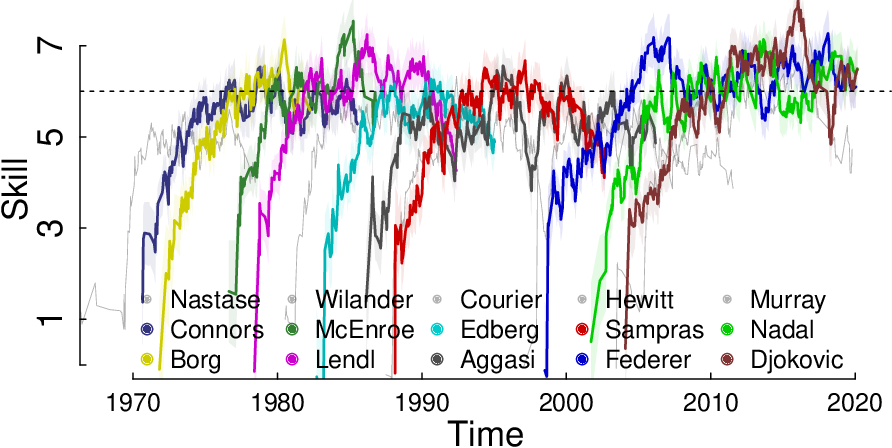
\includegraphics[page={1},width=.8\linewidth]{figures/atp_trueskill}
  \caption{ATP TrueSkill}
  \label{atp_trueskill}
\end{figure}


\subsection{\en{Gaussian product}\es{Producto de gaussianas}}\label{multiplicacion_normales}

\en{The problem we must solve is}
\es{El problema que tenemos que resolver es}
\begin{equation}
 \int \N(x|\mu_1,\sigma_1^2)\N(x|\mu_2,\sigma_2^2) dx
\end{equation}
%
\en{By definition}\es{Por defnici\'on},
\begin{equation}
\begin{split}
 \N(x|y,\beta^2)\N(x|\mu,\sigma^2) & = \frac{1}{\sqrt{2\pi}\sigma_1}e^{-\frac{(x-\mu_1)^2}{2\sigma_1^2}} \frac{1}{\sqrt{2\pi}\sigma_2}e^{-\frac{(x-\mu_2)^2}{2\sigma_2^2}}  \\
 & = \frac{1}{2\pi\sigma_1\sigma_2}\text{exp}\Bigg(-\underbrace{\left( \frac{(x-\mu_1)^2}{2\sigma_1^2} + \frac{(x-\mu_2)^2}{2\sigma_2^2} \right)}_{\theta} \Bigg)
\end{split}
\end{equation}
%
\en{Then}\es{Luego},
\begin{equation}
 \theta = \frac{\sigma_2^2(x^2 + \mu_1^2 - 2x\mu_1) + \sigma_1^2(x^2 + \mu_2^2 - 2x\mu_2) }{2\sigma_1^2\sigma_2^2}
\end{equation}
%
\en{We expand and reorder the factors by powers of $x$}
\es{Expando y reordeno los factores por potencias de $x$}
\begin{equation}
 \frac{(\sigma_1^2 + \sigma_2^2) x^2 - (2\mu_1\sigma_2^2 + 2\mu_2\sigma_1^2) x + (\mu_1^2\sigma_2^2 + \mu_2^2\sigma_1^2)}{2\sigma_1^2\sigma_2^2}
\end{equation}
%
\en{We divide the numerator and denominator by the factor of $x^2$}
\es{Divido al numerador y el denominador por el factor de $x^2$}
\begin{equation}
 \frac{x^2 - 2\frac{(\mu_1\sigma_2^2 + \mu_2\sigma_1^2)}{(\sigma_1^2 + \sigma_2^2) } x + \frac{(\mu_1^2\sigma_2^2 + \mu_2^2\sigma_1^2)}{(\sigma_1^2 + \sigma_2^2) }}{2\frac{\sigma_1^2\sigma_2^2}{(\sigma_1^2 + \sigma_2^2)}}
\end{equation}
%
\en{This equation is quadratic in x, and is therefore proportional to a Gaussian density function with standar deviation}
\es{Esta ecuaci\'on es cuadr\'atica en x, y por lo tanto es proporcional a una funci\'on de densidad gausiana con desv\'io}
\begin{equation}
\sigma_{\times} = \sqrt{\frac{\sigma_1^2\sigma_2^2}{\sigma_1^2+\sigma_2^2}}
\end{equation}
%
\en{and mean}
\es{y media}
\begin{equation}
 \mu_{\times} = \frac{(\mu_1\sigma_2^2 + \mu_2\sigma_1^2)}{(\sigma_1^2 + \sigma_2^2) }
\end{equation}
%
\en{Since a term $\varepsilon = 0$ can be added to complete the square in $\theta$, this proof is sufficient when no normalization is needed. }%
\es{Dado que un t\'ermino $\varepsilon = 0$ puede ser agregado para completar el cuadrado en $\theta$, esta prueba es suficiente cuando no se necesita una normalizaci\'on. }%
%
\begin{equation}
 \varepsilon = \frac{\mu_{\times}^2-\mu_{\times}^2}{2\sigma_{\times}^2} = 0
\end{equation}
%
\en{By adding this term to $\theta$ we obtain}\es{Al agregar este t\'ermino a $\theta$ tenemos}
\begin{equation}
 \theta = \frac{x^2 - 2\mu_{\times}x + \mu_{\times}^2 }{2\sigma_{\times}^2} + \underbrace{\frac{ \frac{(\mu_1^2\sigma_2^2 + \mu_2^2\sigma_1^2)}{(\sigma_1^2 + \sigma_2^2) } - \mu_{\times}^2}{2\sigma_{\times}^2}}_{\varphi}
\end{equation}
%
\en{Reorganizing}\es{Reorganizando} $\varphi$
\begin{equation}
\begin{split}
\varphi & = \frac{\frac{(\mu_1^2\sigma_2^2 + \mu_2^2\sigma_1^2)}{(\sigma_1^2 + \sigma_2^2) } - \left(\frac{(\mu_1\sigma_2^2 + \mu_2\sigma_1^2)}{(\sigma_1^2 + \sigma_2^2) }\right)^2 }{2\frac{\sigma_1^2\sigma_2^2}{\sigma_1^2+\sigma_2^2}}  \\
& = \frac{(\sigma_1^2 + \sigma_2^2)(\mu_1^2\sigma_2^2 + \mu_2^2\sigma_1^2) - (\mu_1\sigma_2^2 + \mu_2\sigma_1^2)^2}{\sigma_1^2 + \sigma_2^2}\frac{1}{2\sigma_1^2\sigma_2^2} \\[0.3cm]
& = \frac{(\mu_1^2\sigma_1^2\sigma_2^2 + \cancel{\mu_2^2\sigma_1^4} + \bcancel{\mu_1^2\sigma_2^4} + \mu_2^2\sigma_1^2\sigma_2^2) - (\bcancel{\mu_1^2\sigma_2^4} + 2\mu_1\mu_2\sigma_1^2\sigma_2^2 + \cancel{\mu_2^2\sigma_1^4} )}{\sigma_1^2 + \sigma_2^2}  \frac{1}{2\sigma_1^2\sigma_2^2} \\[0.3cm]
& = \frac{(\sigma_1^2\sigma_2^2)(\mu_1^2 + \mu_2^2 - 2\mu_1\mu_2)}{\sigma_1^2 + \sigma_2^2}\frac{1}{2\sigma_1^2\sigma_2^2} = \frac{\mu_1^2 + \mu_2^2 - 2\mu_1\mu_2}{2(\sigma_1^2 + \sigma_2^2)} = \frac{(\mu_1 - \mu_2)^2}{2(\sigma_1^2 + \sigma_2^2)}
\end{split}
\end{equation}
%
\en{Then}\es{Luego},
\begin{equation}
 \theta = \frac{(x-\mu_{\times})^2}{2\sigma_{\times}^2} + \frac{(\mu_1 - \mu_2)^2}{2(\sigma_1^2 + \sigma_2^2)}
\end{equation}
%
\en{Putting $\theta$ in place}\es{Colocando $\theta$ en su lugar}
\begin{equation}
\begin{split}
 \N(x|y,\beta^2)\N(x|\mu,\sigma^2) & = \frac{1}{2\pi\sigma_1\sigma_2}\text{exp}\Bigg(-\underbrace{\left( \frac{(x-\mu_{\times})^2}{2\sigma_{\times}^2} + \frac{(\mu_1 - \mu_2)^2}{2(\sigma_1^2 + \sigma_2^2)} \right)}_{\theta} \Bigg) \\
 & = \frac{1}{2\pi\sigma_1\sigma_2}\text{exp}\left(  - \frac{(x-\mu_{\times})^2}{2\sigma_{\times}^2} \right) \text{exp} \left( - \frac{(\mu_1 - \mu_2)^2}{2(\sigma_1^2 + \sigma_2^2)} \right)
\end{split}
\end{equation}
%
\en{Multiplying by}\es{Multiplicando por} $\sigma_{\times}\sigma_{\times}^{-1}$
\begin{equation}
\overbrace{\frac{\cancel{\sigma_1\sigma_2}}{\sqrt{\sigma_1^2+\sigma_2^2}}}^{\sigma_{\times}} \frac{1}{\sigma_{\times}} \frac{1}{2\pi\cancel{\sigma_1\sigma_2}}\text{exp}\left(  - \frac{(x-\mu_{\times})^2}{2\sigma_{\times}^2} \right) \text{exp} \left( - \frac{(\mu_1 - \mu_2)^2}{2(\sigma_1^2 + \sigma_2^2)} \right)
\end{equation}
%
\en{Then}\es{Luego},
\begin{equation}
 \frac{1}{\sqrt{2\pi}\sigma_{\times}}\text{exp}\left(  - \frac{(x-\mu_{\times})^2}{2\sigma_{\times}^2} \right) \frac{1}{\sqrt{2\pi(\sigma_1^2+\sigma_2^2)}} \text{exp} \left( - \frac{(\mu_1 - \mu_2)^2}{2(\sigma_1^2 + \sigma_2^2)} \right)
\end{equation}
%
\en{Going back to the integral}\es{Retonando a la integral}
\begin{equation}
\begin{split}
I & = \int \N(x|\mu_{\times},\sigma_{\times}^2) \overbrace{\N(\mu_1|\mu_2,\sigma_1^2 + \sigma_2^2)}^{\text{Escalar independiente de x}} dx \\[0.3cm]
& = \N(\mu_1|\mu_2,\sigma_1^2 + \sigma_2^2) \underbrace{\int \N(x|\mu_{\times},\sigma_{\times}^2)  dx}_{\text{Integra 1}} \\
& = \N(\mu_1|\mu_2,\sigma_1^2 + \sigma_2^2)
\end{split}
\end{equation}

\subsection{\en{Sum of $n$ Gaussians}\es{Suma de $n$ gaussianas}}\label{suma_normales_induccion}

\en{Proof by induction,}
\es{Demostración por inducción,}

\paragraph{\en{Base case}\es{Casos base}}
%
\begin{equation}
\begin{split}
 P(1) := \int \delta(t_1 = x_1) \N(x_1|\mu_1,\sigma_1^2) dx_1 = \N(t_1|\mu_1,\sigma_1^2)
\end{split}
\end{equation}
%
\en{The proposition $P(1)$ is true given the properties of the delta Dirac function. }%
\es{La proposición $P(1)$ es verdadera dada las propiedades de la función delta de dirac. }%
\begin{equation}\label{eq:induccion_2}
 \begin{split}
P(2) & := \iint \delta(t_2 = x_1 + x_2) \N(x_1|\mu_1, \sigma_1^2)\N(x_2|\mu_2, \sigma_2^2) dx_1dx_2 \\
 & \overset{\ref{eq:induccion_2}.1}{=} \int \N(x_1|\mu_1, \sigma_1^2) \N(t_2 - x_1|\mu_2, \sigma_2^2) dx_1   \\
 & \overset{\ref{eq:induccion_2}.2}{=} \int \N(x_1|\mu_1, \sigma_1^2) \N(x_1|t_2 - \mu_2, \sigma_2^2) dx_1 \\
 & \overset{*}{=} \int \underbrace{N(t_2|\mu_1+\mu_2,\sigma_1^2 + \sigma_2^2)}_{\text{const.}} \underbrace{\N(x_1|\mu_{*},\sigma_{*}^2) dx_1}_{1} \\
 & = \N(t_2|\mu_1+\mu_2,\sigma_1^2 + \sigma_2^2)
 \end{split}
 \end{equation}
%
 \en{Where $\overset{\ref{eq:induccion_2}.1}{=}$ is valid for the properties of the dirac delta function, $\overset{\ref{eq:induccion_2}.2}{=}$ is valid for the symmetry of the Gaussians, and $\overset{*}{=}$ is valid by de proof at section~\ref{multiplicacion_normales}. }%
 \es{Donde $\overset{\ref{eq:induccion_2}.1}{=}$ vale por las propiedades de la función delta de dirac, $\overset{\ref{eq:induccion_2}.2}{=}$ vale por la simetría de las gaussianas, y $\overset{*}{=}$ vale por la demostraci\'on de miltiplicaci\'on de normales en la secci\'on~\ref{multiplicacion_normales}. }%
 %
 \en{Therefore, $P(2)$ is valid. }%
 \es{Luego, vale $P(2)$. }%


\paragraph{\en{Inductive step}\es{Paso inductivo}} $P(n) \Rightarrow P(n+1)$

\en{Given}\es{Dado},
\begin{equation}
 P(n) :=\int \dots \int \delta(t_n= \sum_{i=1}^n x_i ) \left( \prod_{i=1}^n \N(x_i|\mu_i,\sigma_i^2) \right) dx_1 \dots dx_n = \N(t|\sum_{i=1}^n \mu_i,\sum_{i=1}^n \sigma_i^2 )
\end{equation}
%
\en{We want to see that $P(n+1)$ is valid. }%
\es{Queremos ver que $P(n+1)$ es válida. }%
%
\begin{equation}
 P(n+1) := \int \dots \int \delta(t_{n+1}=x_{n+1} + \sum_{i=1}^{n} x_i ) \left( \prod_{i=1}^{n} \N(x_i|\mu_i,\sigma_i^2) \right) \N(x_{n+1}|\mu_{n+1},\sigma_{n+1}^2) dx_1 \dots dx_{n} dx_{n+1}
\end{equation}
%
\en{By independence}
\es{Por independencia}
\begin{equation}
 \int \N(x_{n+1}|\mu_{n+1},\sigma_{n+1}^2) \left( \int \dots \int \delta(t_{n+1}= x_{n+1} + \sum_{i=1}^{n} x_i ) \left( \prod_{i=1}^{n} \N(x_i|\mu_i,\sigma_i^2) \right)  dx_1 \dots dx_{n}\right) dx_{n+1}
\end{equation}
%
\en{By inductive hypothesis}
\es{Por hip\'otesis inductiva}
\begin{equation}
 \int \N(x_{n+1}|\mu_{n+1},\sigma_{n+1}^2) \N(t_{n+1}-x_{n+1}|\sum_{i=1}^n \mu_i,\sum_{i=1}^n \sigma_i^2) dx_{n+1}
\end{equation}
%
\en{By de proof of section~\ref{multiplicacion_normales}}
\es{Por la demostraci\'on de la secci\'on~\ref{multiplicacion_normales}}
\begin{equation}
  \N(t_{n+1}|\mu_{n+1}+\sum_{i=1}^{n} \mu_i,\sigma_{n+1}^2 \sum_{i=1}^n \sigma_i^2) dx_{n+1}
\end{equation}
%
\en{Therefore, $P(n+1)$ is valid}
\es{Luego, $P(n+1)$ es válida. }%

\subsection{\en{A Gaussian multiplied by an cumulative Gaussian.}\es{Gaussiana por acumulada de Gaussiana.}}

\en{We want to solve the integral}
\es{Queremos resolver la integral}
\begin{equation}
 f(x) = \int \N(y;\mu_1,\sigma_1^2)\Phi(y+x;\mu_2,\sigma_2^2) dy
\end{equation}
%
\en{To do so, we take the derivative of the function}\es{Para ello trabajamos con la drivada} $\frac{\partial}{\partial x}f(x) = \theta(x)$,
\begin{equation}
 \theta(x) = \frac{\partial}{\partial x}\int \N(y;\mu_1,\sigma_1^2)\Phi(y+x|\mu_2,\sigma_2^2) dy
\end{equation}
%
\begin{equation}
 \theta(x) = \int \N(y|\mu_1,\sigma_1^2)\frac{\partial}{\partial x}\Phi(y+x|\mu_2,\sigma_2^2) dy
\end{equation}
%
\en{The derivative of $\Phi$ is indeed a Gaussian,}
\es{La derivada de $\Phi$ es justamente una Gaussiana,}
\begin{equation}
\begin{split}
\theta(x) & = \int \N(y|\mu_1,\sigma_1^2)\N(y+x|\mu_2,\sigma_2^2) dy \\
& = \int \N(y|\mu_1,\sigma_1^2)\N(y|\mu_2-x,\sigma_2^2) dy
\end{split}
\end{equation}
%
\en{By the proof at section~\ref{multiplicacion_normales} we know}
\es{Por la demostraci\'on de la secci\'on~\ref{multiplicacion_normales} sabemos}
\begin{equation}
 \theta(x) = \N(\mu_1| \mu_2 - x, \sigma_1^2 + \sigma_2^2)
\end{equation}
%
\en{By symmetry}
\es{Por simetr\'ia}
\begin{equation}
 \theta(x) = \N(x| \mu_2 - \mu_1, \sigma_1^2 + \sigma_2^2)
\end{equation}
%
\en{Returning to $f(x)$}
\es{Retornando a $f(x)$}
\begin{equation}
 f(x) = \Phi(x| \mu_2 - \mu_1, \sigma_1^2 + \sigma_2^2)
\end{equation}

\subsection{\en{Gaussian division}\es{Division de gaussianas}}\label{sec:division_normales}

\begin{equation}
\kappa = \frac{\N(x|\mu_f,\sigma_f^2)}{\N(x|\mu_g,\sigma_g^2)} = \N(x|\mu_f,\sigma_f^2)\N(x|\mu_g,\sigma_g^2)^{-1}
\end{equation}
%
\en{By definition}\es{Por definici\'on}
\begin{equation}
\begin{split}
\kappa & = \frac{1}{\sqrt{2\pi}\sigma_f}e^{-\left(\frac{(x-\mu_f)^2}{2\sigma_f^2}\right)} \left( \frac{1}{\sqrt{2\pi}\sigma_g}e^{-\left(\frac{(x-\mu_g)^2}{2\sigma_g^2}\right)} \right)^{-1} \\[0.3cm]
& = \frac{1}{\cancel{\sqrt{2\pi}}\sigma_f}e^{-\left(\frac{(x-\mu_f)^2}{2\sigma_f^2}\right)} \frac{\cancel{\sqrt{2\pi}}\sigma_g}{1} e^{\left(\frac{(x-\mu_g)^2}{2\sigma_g^2}\right)} \\[0.3cm]
& = \frac{\sigma_g}{\sigma_f}\text{exp}\Bigg(-\underbrace{\Big(\frac{(x-\mu_f)^2}{2\sigma_f^2} - \frac{(x-\mu_g)^2}{2\sigma_g^2}\Big)}_{\theta}\Bigg)
\end{split}
\end{equation}
%
\en{Reorganizing}\es{Reorganizando} $\theta$
\begin{equation}
\begin{split}
 \theta & = \frac{(x-\mu_f)^2}{2\sigma_f^2} - \frac{(x-\mu_g)^2}{2\sigma_g^2} = \frac{\sigma_g^2(x-\mu_f)^2 - \sigma_f^2(x-\mu_g)^2}{2\sigma_f^2\sigma_g^2} \\[0.3cm]
 & = \frac{\sigma_g^2(x^2+\mu_f^2-2\mu_fx) - \sigma_f^2(x^2+\mu_g^2-2\mu_gx)}{2\sigma_f^2\sigma_g^2}
\end{split}
\end{equation}
%
\en{We expand and sort terms based on $x$,}\es{Expandimos y ordenamos en base $x$,}
%
\begin{equation}
\begin{split}
 \theta & = \left((\sigma_g^2 - \sigma_f^2)x^2 - 2(\sigma_g^2\mu_f - \sigma_f^2\mu_g)x + (\sigma_g^2\mu_f^2 - \sigma_f^2\mu_g^2 )\right) \frac{1}{2\sigma_f^2\sigma_g^2} \\[0.3cm]
 & = \left(x^2 - \frac{2(\sigma_g^2\mu_f - \sigma_f^2\mu_g)}{(\sigma_g^2 - \sigma_f^2)}x + \frac{(\sigma_g^2\mu_f^2 - \sigma_f^2\mu_g^2 )}{(\sigma_g^2 - \sigma_f^2)}\right) \frac{(\sigma_g^2 - \sigma_f^2)}{2\sigma_f^2\sigma_g^2}
\end{split}
\end{equation}
%
\en{This is quadratic in $x$. Since a term $\varepsilon=0$ independent of $x$ can be added to complete the square in $\theta$, this test is sufficient to determine the mean and variance when it is not necessary to normalize. }%
\es{Esto es cuadr\'atico en x. Dado que un t\'ermino $\varepsilon=0$, independiente de $x$ puede ser agregado para completar el cuadrado en $\theta$, esta prueba es suficiente para dterminar la media y la varianza cuando no es necesario normalizar. }%
%
\begin{equation}
 \sigma_{\div} = \sqrt{\frac{\sigma_f^2\sigma_g^2}{(\sigma_g^2 - \sigma_f^2)}}
\end{equation}
%
\begin{equation}
 \mu_{\div} = \frac{(\sigma_g^2\mu_f - \sigma_f^2\mu_g)}{(\sigma_g^2 - \sigma_f^2)}
\end{equation}
%
\en{adding}\es{agregado} $\varepsilon = \frac{\mu_{\div}^2-\mu_{\div}^2}{2\sigma_{\div}^2} = 0$
\begin{equation}
\theta = \frac{x^2 - 2\mu_{\div}x + \mu_{\div}^2 }{2\sigma_{\div}^2} + \underbrace{ \frac{ \frac{(\sigma_g^2\mu_f^2 - \sigma_f^2\mu_g^2)}{(\sigma_g^2 - \sigma_f^2)} - \mu_{\div}^2 }{2\sigma_{\div}^2} }_{\varphi}
\end{equation}

\en{Reorganizing}\es{Reorganizando} $\varphi$
\begin{equation}
\begin{split}
 \varphi & = \left( \frac{(\sigma_g^2\mu_f^2 - \sigma_f^2\mu_g^2)}{(\sigma_g^2 - \sigma_f^2)} - \left(\frac{(\sigma_g^2\mu_f - \sigma_f^2\mu_g)}{(\sigma_g^2 - \sigma_f^2)} \right)^2 \right) \frac{(\sigma_g^2 - \sigma_f^2)}{2\sigma_f^2\sigma_g^2} \\[0.3cm]
 & = \left((\sigma_g^2\mu_f^2 - \sigma_f^2\mu_g^2)(\sigma_g^2 - \sigma_f^2) - \left((\sigma_g^2\mu_f - \sigma_f^2\mu_g) \right)^2 \right) \frac{1}{2\sigma_f^2\sigma_g^2(\sigma_g^2 - \sigma_f^2)} \\[0.3cm]
 & =  \left( \cancel{\sigma_g^4\mu_f^2} - \sigma_f^2\sigma_g^2\mu_f^2 - \sigma_f^2\sigma_g^2\mu_g^2 + \bcancel{\sigma_f^4\mu_g^2} - (\cancel{\sigma_g^4\mu_f^2} + \bcancel{\sigma_f^4\mu_g^2 } - 2\sigma_f^2\sigma_g^2\mu_f\mu_g)\right) \frac{1}{2\sigma_f^2\sigma_g^2(\sigma_g^2 - \sigma_f^2)}
 \end{split}
\end{equation}
%
\en{Canceling}\es{Cancelando} $\sigma_f^2\sigma_g^2$
\begin{equation}
 \varphi = \frac{- \mu_g^2 - \mu_f^2 + 2\mu_f\mu_g}{2(\sigma_g^2 - \sigma_f^2)} = \frac{- (\mu_g - \mu_f)^2}{2(\sigma_g^2 - \sigma_f^2)}
\end{equation}
%
\en{Then}\es{Luego} $\theta$
\begin{equation}
 \theta = \frac{(x - \mu_{\div})^2}{2\sigma_{\div}^2} - \frac{(\mu_g - \mu_f)^2)}{2(\sigma_g^2 - \sigma_f^2)}
\end{equation}

\en{Returning to the original expression}\es{Volviendo a la expresión original}
\begin{equation}
\begin{split}
 \kappa & = \frac{\sigma_g}{\sigma_f}  \, \text{exp}\left(- \frac{(x - \mu_{\div})^2}{2\sigma_{\div}^2} + \frac{(\mu_g - \mu_f)^2)}{2(\sigma_g^2 - \sigma_f^2)}  \right)\\[0.3cm]
 & = \frac{\sigma_g}{\sigma_f} \, \text{exp}\left({-\frac{(x - \mu_{\div})^2}{2\sigma_{\div}^2}}\right) \, \text{exp}\left({\frac{(\mu_g - \mu_f)^2)}{2(\sigma_g^2 - \sigma_f^2)}}\right)
\end{split}
\end{equation}

\en{Multiplying by}\es{Multiplicando por} $\frac{\sqrt{2\pi}}{\sqrt{2\pi}}\frac{\sigma_{\div}}{\sigma_{\div}}\frac{\sqrt{\sigma_g^2 - \sigma_f^2}}{\sqrt{\sigma_g^2 - \sigma_f^2}}=1$,
\begin{equation}
\begin{split}
 \kappa & =  \frac{1}{\sqrt{2\pi}\sigma_{\div}} \, e^{-\frac{(x - \mu_{\div})^2}{2\sigma_{\div}^2}} \, \left( \frac
 {1}{\sqrt{2\pi(\sigma_g^2 - \sigma_f^2)} } e^{-\frac{(\mu_g - \mu_f)^2)}{2(\sigma_g^2 - \sigma_f^2)}} \right)^{-1} \, \frac{\sigma_{\div}}{\sqrt{\sigma_g^2 - \sigma_f^2}}\frac{\sigma_g}{\sigma_f}\\[0.3cm]
 & = \frac{\N\left(x| \mu_{\div},\sigma_{\div}\right)}{\N\left(\mu_g|\mu_f,\sigma_g^2-\sigma_f^2\right)} \frac{\sigma_g^2}{\sigma_g^2 - \sigma_f^2}
\end{split}
\end{equation}




%% -----------------------------------------------------------------------------

\end{document}
